% ==============================================================================
% Monografia de Graduação - Ciência da Computação - Áurea Santos de Oliveira
% Baseado no modelo para Projeto de Graduação do Colegiado (em Português)
% Prof. Vítor E. Silva Souza - NEMO / PPGI | DI / CT / UFES
% Com adaptações feitas pelo Colegiado de Engenharia de Computação / CT / UFES e pela profª. Monalessa Perini Barcellos (NEMO/UFES).
%
% Baseado em abtex2-modelo-trabalho-academico.tex, v-1.9.2 laurocesar
% Copyright 2012-2014 by abnTeX2 group at http://abntex2.googlecode.com/ 
%
% This work may be distributed and/or modified under the conditions of the LaTeX 
% Project Public License, either version 1.3 of this license or (at your option) 
% any later version. The latest version of this license is in
% http://www.latex-project.org/lppl.txt.
%
% IMPORTANTE:
% Instruções encontram-se espalhadas pelo documento. Para facilitar sua leitura,
% tais instruções são precedidas por (*) -- utilize a função localizar do seu
% editor para passar por todas elas.
% ==============================================================================

% Usa o estilo abntex2, configurando detalhes de formatação e hifenização.
\documentclass[
	12pt,				% Tamanho da fonte.
	openright,			% Capítulos começam em página ímpar (insere página vazia caso preciso).
	oneside,			% Para impressão em verso e anverso. Oposto a oneside.
	a4paper,			% Tamanho do papel.
	english,			% Idioma adicional para hifenização.
	french,				% Idioma adicional para hifenização.
	spanish,			% Idioma adicional para hifenização.
	brazil				% O último idioma é o principal do documento.
	]{abntex2}



%%% Importação de pacotes. %%%

% Conserta o erro "No room for a new \count". 
% O comando \reserveinserts deve ser comentado ou não, dependendo da versão do LaTeX.
\usepackage{etex}
%\reserveinserts{28}

% Usa a fonte Latin Modern.
\usepackage{lmodern}

% Seleção de códigos de fonte.
\usepackage[T1]{fontenc}

% Codificação do documento em Unicode.
\usepackage[utf8]{inputenc}

% Usado pela ficha catalográfica.
\usepackage{lastpage}

% Indenta o primeiro parágrafo de cada seção.
\usepackage{indentfirst}

% Controle das cores.
\usepackage[usenames,dvipsnames]{xcolor}

% Inclusão de gráficos.
\usepackage{graphicx}

% Tabularx package: melhor controle de leiaute de tabelas.
\usepackage{tabularx}

% Inclusão de páginas em PDF diretamente no documento (para uso nos apêndices).
\usepackage{pdfpages}

% Para melhorias de justificação.
\usepackage{microtype}

% Citações padrão ABNT.
\usepackage[brazilian,hyperpageref]{backref}
\usepackage[alf]{abntex2cite}	
\renewcommand{\backrefpagesname}{Citado na(s) página(s):~}		% Usado sem a opção hyperpageref de backref.
\renewcommand{\backref}{}										% Texto padrão antes do número das páginas.
\renewcommand*{\backrefalt}[4]{									% Define os textos da citação.
	\ifcase #1
		Nenhuma citação no texto.
	\or
		Citado na página #2.
	\else
		Citado #1 vezes nas páginas #2.
	\fi}

% \rm is deprecated and should not be used in a LaTeX2e document
% http://tex.stackexchange.com/questions/151897/always-textrm-never-rm-a-counterexample
\renewcommand{\rm}{\textrm}

% Inclusão de símbolos não padrão.
\usepackage{amssymb}
\usepackage{eurosym}

% Para utilizar \eqref para referenciar equações.
\usepackage{amsmath}

% Permite mostrar figuras muito largas em modo paisagem com \begin{sidewaysfigure} ao invés de \begin{figure}.
\usepackage{rotating}

% Permite customizar listas enumeradas/com marcadores.
\usepackage{enumitem}

% Permite inserir hiperlinks com \url{}.
\usepackage{bigfoot}
\usepackage{hyperref}
\usepackage{xurl}  % permite quebrar URLs longas nas referências

% Permite usar o comando \hl{} para evidenciar texto com fundo amarelo. Útil para chamar atenção a itens a fazer.
\usepackage{soulutf8}

% Colorinlistoftodos package: to insert colored comments so authors can collaborate on the content.
\usepackage[colorinlistoftodos, textwidth=20mm, textsize=footnotesize]{todonotes}
\newcommand{\aluno}[1]{\todo[author=\textbf{Aluno},color=green!30,caption={},inline]{#1}}
\newcommand{\professor}[1]{\todo[author=\textbf{Professor},color=red!30,caption={},inline]{#1}}

% Permite inserir espaço em branco condicional (incluído no texto final só se necessário) em macros.
\usepackage{xspace}

% Permite incluir listagens de código com o comando \lstinputlisting{}.
\usepackage{listings}
\usepackage{caption}
\DeclareCaptionFont{white}{\color{white}}
\DeclareCaptionFormat{listing}{\colorbox{gray}{\parbox{\textwidth}{#1#2#3}}}
\captionsetup[lstlisting]{format=listing,labelfont=white,textfont=white}
\renewcommand{\lstlistingname}{Listagem}
\definecolor{mygray}{rgb}{0.5,0.5,0.5}
\lstset{
	basicstyle=\scriptsize,
	breaklines=true,
	numbers=left,
	numbersep=5pt,
	numberstyle=\tiny\color{mygray}, 
	rulecolor=\color{black},
	showstringspaces=false,
	tabsize=2,
    inputencoding=utf8,
    extendedchars=true,
    literate=%
    {é}{{\'{e}}}1
    {è}{{\`{e}}}1
    {ê}{{\^{e}}}1
    {ë}{{\¨{e}}}1
    {É}{{\'{E}}}1
    {Ê}{{\^{E}}}1
    {û}{{\^{u}}}1
    {ù}{{\`{u}}}1
    {â}{{\^{a}}}1
    {à}{{\`{a}}}1
    {á}{{\'{a}}}1
    {ã}{{\~{a}}}1
    {Á}{{\'{A}}}1
    {Â}{{\^{A}}}1
    {Ã}{{\~{A}}}1
    {ç}{{\c{c}}}1
    {Ç}{{\c{C}}}1
    {õ}{{\~{o}}}1
    {ó}{{\'{o}}}1
    {ô}{{\^{o}}}1
    {Õ}{{\~{O}}}1
    {Ó}{{\'{O}}}1
    {Ô}{{\^{O}}}1
    {î}{{\^{i}}}1
    {Î}{{\^{I}}}1
    {í}{{\'{i}}}1
    {Í}{{\'{I}}}1
    {ú}{{\'{u}}}1
    {Ú}{{\'{U}}}1
    {ü}{{\"{u}}}1
    {º}{{\textordmasculine}}1
    {ª}{{\textordfeminine}}1
    {§}{{\S}}1
}



%%% Definição de variáveis. %%%

% (*) Substituir os textos abaixo com as informações apropriadas.
\titulo{GraphRAG Aplicado à Legislação Consumerista: uma Prova de Conceito para Indexação e Consulta em Grafo do Código de Defesa do Consumidor}
\autor{Áurea Santos de Oliveira}
\local{Vitória, ES}
\data{2026}
\orientador{Prof. Dr. João Paulo Almeida}
%\coorientador{Nome do Co-orientador}
\instituicao{
  Universidade Federal do Espírito Santo -- UFES
  \par
  Centro Tecnológico
  \par
  Colegiado do Curso de Ciência da Computação}
\tipotrabalho{Monografia (PG)}

% Preâmbulo (tipo do trabalho, objetivo, nome da instituição, área de concentração, etc.).
\preambulo{Monografia apresentada ao Curso de Ciência da Computação do Centro Tecnológico da Universidade Federal do Espírito Santo, como requisito parcial para obtenção do Grau de Bacharel em Ciência da Computação.}

% Macros específicas do trabalho.
% (*) Inclua aqui termos que são utilizados muitas vezes e que demandam formatação especial.
% Os exemplos abaixo incluem i* (substituindo o asterisco por uma estrela) e Java com TM em superscript.
% Use sempre \xspace para que o LaTeX inclua espaço em branco após a macro somente quando necessário.
\newcommand{\latex}{\LaTeX\xspace}
\newcommand{\graphrag}{GraphRAG\xspace}
\newcommand{\cdc}{CDC\xspace}
\newcommand{\eng}[1]{\textit{#1}}             % termo em inglês
\newcommand{\codeus}{\textunderscore\allowbreak}
\newcommand{\code}[1]{{\ttfamily\let\_\codeus #1}}  % nomes de arquivos, opções e trechos de código (quebra após _)
\newcommand{\pendente}[1]{{\color{BrickRed}#1}} % trechos a completar

% Diagramas.
\usepackage{tikz}
\usetikzlibrary{arrows.meta,positioning,shapes.geometric,shapes.multipart,fit,backgrounds,calc}
% Tabelas longas e colunas com quebra de linha.
\usepackage{longtable}
\usepackage{float}
\usepackage{needspace}  % evita título de seção isolado no fim da página  % [H]: mantém a figura/tabela exatamente onde está no texto
\usepackage{booktabs}
\usepackage{array}
\newcolumntype{L}[1]{>{\raggedright\arraybackslash}p{#1}}




%%% Configurações finais de aparência. %%%

% Altera o aspecto da cor azul.
\definecolor{blue}{RGB}{41,5,195}

% Informações do PDF.
\makeatletter
\hypersetup{
	pdftitle={\@title}, 
	pdfauthor={\@author},
	pdfsubject={\imprimirpreambulo},
	pdfcreator={LaTeX with abnTeX2},
	pdfkeywords={abnt}{latex}{abntex}{abntex2}{trabalho acadêmico}, 
	colorlinks=true,				% Colore os links (ao invés de usar caixas).
	linkcolor=blue,					% Cor dos links.
	citecolor=blue,					% Cor dos links na bibliografia.
	filecolor=magenta,				% Cor dos links de arquivo.
	urlcolor=blue,					% Cor das URLs.
	bookmarksdepth=4
}
\makeatother

% Posicionamento de figuras e tabelas: permite mais flutuantes por página e reduz páginas
% com espaço em branco.
\renewcommand{\topfraction}{0.9}
\renewcommand{\bottomfraction}{0.8}
\renewcommand{\textfraction}{0.07}
\renewcommand{\floatpagefraction}{0.8}
\setcounter{topnumber}{3}
\setcounter{bottomnumber}{2}
\setcounter{totalnumber}{5}

% Listas mais compactas.
\setlist{itemsep=1pt, topsep=3pt, parsep=1pt}

% Espaçamentos entre linhas e parágrafos.
\setlength{\parindent}{1.3cm}
\setlength{\parskip}{0.2cm}



%%% Páginas iniciais do documento: capa, folha de rosto, ficha, resumo, tabelas, etc. %%%

% Compila o índice.
\makeindex

% Inicia o documento.
\begin{document}

% Brasão da instituição.
\begin{figure}
	\centering
	
\includegraphics[width=.20\textwidth]{figuras/brasao.jpg} 
	\label{fig-brasao}
\end{figure}

\begin{center}
	\textbf{\textsf{UNIVERSIDADE FEDERAL DO ESPÍRITO SANTO}}
	
	\textbf{\textsf{CENTRO TECNOLÓGICO}}
	
	\textbf{\textsf{COLEGIADO DO CURSO DE CIÊNCIA DA COMPUTAÇÃO}}
	
	\large{\textbf{\textsf{  }}}
	
	\large{\textbf{\textsf{  }}}
\end{center}

% Retira espaço extra obsoleto entre as frases.
\frenchspacing

% Capa do trabalho.
\imprimircapa

% Folha de rosto (o * indica que haverá a ficha bibliográfica).
\imprimirfolhaderosto*


% Ficha catalográfica.
% (*) Escolher entre as versões de ficha catalográfica abaixo (comente aquela que não quiser usar).

% Versão 1: caso a biblioteca da sua universidade lhe forneça um PDF (adequar o nome do arquivo).
% \begin{fichacatalografica}
%     \includepdf{include-fichacatalografica.pdf}
% \end{fichacatalografica}

% Versão 2: caso você tenha que inserir sua própria ficha catalográfica.
% (*) Neste caso, preencher palavras-chave e adicione co-orientador (se houver).
\begin{fichacatalografica}
	\vspace*{\fill}
	\hrule
	\begin{center}
	\begin{minipage}[c]{12.5cm}
	
	\imprimirautor
	
	\hspace{0.5cm} \imprimirtitulo  / \imprimirautor. --
	\imprimirlocal, \imprimirdata-
	
	\hspace{0.5cm} \pageref{LastPage} p. : il. (algumas color.) ; 30 cm.\\
	
	\hspace{0.5cm} \imprimirorientadorRotulo~\imprimirorientador\\
	
	\hspace{0.5cm}
	\parbox[t]{\textwidth}{\imprimirtipotrabalho~--~\imprimirinstituicao,
	\imprimirdata.}\\
	
	\hspace{0.5cm}
		1. GraphRAG.
		2. Geração aumentada por recuperação.
		3. Grafos de conhecimento.
		4. Código de Defesa do Consumidor.
		I. Almeida, João Paulo.
		II. Universidade Federal do Espírito Santo.
		IV. \imprimirtitulo \\ 			
	
	\hspace{8.75cm} CDU 02:141:005.7\\
	
	\end{minipage}
	\end{center}
	\hrule
\end{fichacatalografica}


% Folha de aprovação.
% (*) Escolher entre as versões de ficha catalográfica abaixo (comente aquela que não quiser usar).

% Versão 1: cópia digitalizada da folha de aprovação assinada pela banca.
% \includepdf{include-folhadeaprovacao.pdf}

% Versão 2: folha de aprovação em branco.
% (*) Ajustar a data e os nomes dos participantes da banca.
\begin{folhadeaprovacao}
  \begin{center}
    {\ABNTEXchapterfont\large\imprimirautor}
    \vspace*{\fill}\vspace*{\fill}
    \begin{center}
      \ABNTEXchapterfont\bfseries\Large\imprimirtitulo
    \end{center}
    \vspace*{\fill}
    \hspace{.45\textwidth}
    \begin{minipage}{.5\textwidth}
        \imprimirpreambulo
    \end{minipage}%
    \vspace*{\fill}
   \end{center}
   Trabalho aprovado. \imprimirlocal, (dia) de (mês) de (ano):
   \assinatura{\textbf{\imprimirorientador} \\ Orientador}
   \assinatura{\textbf{Nome do Membro da Banca} \\ Nome da Instituição}
   \assinatura{\textbf{Nome do Membro da Banca} \\ Nome da Instituição}
   %\assinatura{\textbf{Nome do Membro da Banca} \\ Nome da Instituição}
   %\assinatura{\textbf{Nome do Membro da Banca} \\ Nome da Instituição}
   \begin{center}
    \vspace*{0.5cm}
    {\large\imprimirlocal}
    \par
    {\large\imprimirdata}
    \vspace*{1cm}
  \end{center}  
\end{folhadeaprovacao}


% Dedicatória, agradecimentos e epígrafe.
% (*) A escrever pela autora. Descomente os blocos quando tiver o texto.
% \begin{dedicatoria}
%    \vspace*{\fill}
%    \centering
%    \noindent
%    \textit{Texto da dedicatória.} \vspace*{\fill}
% \end{dedicatoria}
%
% \begin{agradecimentos}
% Texto dos agradecimentos.
% \end{agradecimentos}
%
% \begin{epigrafe}
%     \vspace*{\fill}
% 	\begin{flushright}
% 		\textit{``Texto da epígrafe.''\\ (Autor)}
% 	\end{flushright}
% \end{epigrafe}


% Resumo em português.
% (*) Escrever resumo e palavras-chave.
\setlength{\absparsep}{18pt}
\begin{resumo}
% ==============================================================================
% Monografia - Áurea Santos de Oliveira
% Resumo (incluído dentro do ambiente resumo do arquivo principal)
% ==============================================================================
\aluno{Versão preliminar do resumo. Completar com os resultados da avaliação (Capítulo~\ref{sec-avaliacao}) e ajustar para no máximo 500 palavras.}

Sistemas de geração aumentada por recuperação (\textit{Retrieval-Augmented Generation} -- RAG) permitem que modelos de linguagem de grande porte respondam perguntas com base em uma base de conhecimento externa. Na abordagem vetorial tradicional, porém, o texto é recuperado em fragmentos isolados, o que limita respostas que dependem de relações entre partes distantes do corpus -- situação típica de textos legislativos, nos quais artigos remetem uns aos outros e estabelecem definições, exceções e consequências. Este trabalho investiga o GraphRAG, \textit{framework} de código aberto da Microsoft que constrói, com o auxílio de um modelo de linguagem, um grafo de conhecimento a partir do texto, agrupa suas entidades em comunidades hierárquicas e gera relatórios sobre essas comunidades, oferecendo quatro modalidades de consulta: local, global, DRIFT e básica (vetorial). Como prova de conceito, o Código de Defesa do Consumidor (Lei nº 8.078/1990) foi estruturado em um registro por artigo, com sua hierarquia e situação normativa, e indexado com o GraphRAG 3.1.0 utilizando modelos de linguagem em nuvem, uma taxonomia de catorze tipos de entidade definida para o domínio e \textit{prompts} de extração ajustados ao corpus. O índice resultante contém 1.373 entidades, 6.885 relações e 369 comunidades. Foi desenvolvida ainda uma aplicação web, executada em contêineres Docker, que permite explorar o grafo, realizar consultas nas quatro modalidades acompanhando cada etapa da recuperação (contexto recuperado, \textit{prompt} enviado ao modelo, resposta e consumo de \textit{tokens}), destacar no grafo a parte utilizada como contexto e registrar todo o histórico em banco de dados para a avaliação. Durante o desenvolvimento foram identificados e contornados defeitos da biblioteca que afetam diretamente a comparação entre as modalidades, entre eles uma falha que faz a busca básica retornar respostas vazias quando usada programaticamente. \pendente{[Resultados da avaliação comparativa entre as modalidades do GraphRAG e o \textit{baseline} vetorial.]}

\textbf{Palavras-chave}: GraphRAG. Geração aumentada por recuperação. Grafos de conhecimento. Modelos de linguagem. Código de Defesa do Consumidor.

\end{resumo}

% Insere lista de ilustrações.
\pdfbookmark[0]{\listfigurename}{lof}
\listoffigures*
\cleardoublepage

% Insere lista de tabelas.
\pdfbookmark[0]{\listtablename}{lot}
\listoftables*
\cleardoublepage

% Lista de abreviaturas e siglas.
% (*) Preencher com as siglas usadas ao longo do texto e seus significados.
\begin{siglas}
  \item[API] \textit{Application Programming Interface}
  \item[CDC] Código de Defesa do Consumidor (Lei nº 8.078/1990)
  \item[CLI] \textit{Command Line Interface}
  \item[CORS] \textit{Cross-Origin Resource Sharing}
  \item[DRIFT] \textit{Dynamic Reasoning and Inference with Flexible Traversal}
  \item[HyDE] \textit{Hypothetical Document Embeddings}
  \item[HTTP] \textit{Hypertext Transfer Protocol}
  \item[JSON] \textit{JavaScript Object Notation}
  \item[LLM] \textit{Large Language Model}
  \item[ORM] \textit{Object-Relational Mapping}
  \item[PLN] Processamento de Linguagem Natural
  \item[PoC] \textit{Proof of Concept} (prova de conceito)
  \item[RAG] \textit{Retrieval-Augmented Generation}
  \item[REST] \textit{Representational State Transfer}
  \item[SPA] \textit{Single Page Application}
  \item[SQL] \textit{Structured Query Language}
  \item[SSE] \textit{Server-Sent Events}
  \item[YAML] \textit{YAML Ain't Markup Language}
\end{siglas}

% Insere o sumário.
\pdfbookmark[0]{\contentsname}{toc}
\tableofcontents*
\cleardoublepage



%%% Início da parte de conteúdo do documento. %%%

% Marca o início dos elementos textuais.
\textual

% Inclusão dos capítulos.
% (*) Para facilitar a organização, os capítulos foram divididos em arquivo separados e colocados dentro da.
% pasta capitulos/. Caso o aluno prefira trabalhar com um só arquivo, basta substituir os comandos \include 
% pelos conteúdos dos arquivos que estão sendo incluídos, excluindo a pasta capitulos/ em seguida.
% ==============================================================================
% Monografia - Áurea Santos de Oliveira
% Capítulo 1 - Introdução
% ==============================================================================
\chapter{Introdução}
\label{sec-intro}

Modelos de linguagem de grande porte (\textit{Large Language Models} -- LLMs) \cite{vaswani2017attention, brown2020language} tornaram-se capazes de responder perguntas em linguagem natural sobre praticamente qualquer assunto. Seu conhecimento, no entanto, é limitado ao que estava presente nos dados de treinamento e está sujeito a erros factuais apresentados com aparente segurança, fenômeno conhecido como alucinação \cite{ji2023survey}. Para aplicações em que a resposta precisa estar fundamentada em um conjunto específico de documentos -- como uma lei --, a abordagem mais utilizada é a geração aumentada por recuperação (\textit{Retrieval-Augmented Generation} -- RAG) \cite{lewis2020retrieval}: no momento da consulta, os trechos mais relevantes de uma base de conhecimento externa são recuperados e inseridos no contexto do modelo, que gera a resposta a partir deles.

Na forma mais comum de RAG, o texto é dividido em fragmentos (\textit{chunks}), cada fragmento é convertido em um vetor numérico (\textit{embedding}) e, na consulta, recuperam-se os fragmentos cujos vetores são mais similares ao vetor da pergunta \cite{gao2023retrieval}. Essa estratégia funciona bem quando a resposta está concentrada em poucos trechos, mas apresenta limitações quando o conhecimento tem estrutura fortemente relacional e a resposta depende de conectar informações dispersas pelo corpus. Essa situação é recorrente em textos legislativos: artigos remetem uns aos outros, estabelecem definições usadas em outros pontos da lei, preveem exceções e consequências em dispositivos distintos e organizam-se em uma hierarquia de títulos, capítulos e seções que também carrega significado.

O \textit{framework} GraphRAG, desenvolvido pela Microsoft Research \cite{edge2024global}, propõe uma alternativa a essa limitação. Em vez de recuperar apenas fragmentos semanticamente similares, o GraphRAG utiliza um LLM para extrair do corpus um grafo de conhecimento -- entidades e relações entre elas --, agrupa as entidades em comunidades hierárquicas por meio de um algoritmo de detecção de comunidades e gera relatórios textuais que resumem cada comunidade. Essas estruturas permitem modalidades de consulta que não existem no RAG vetorial: buscas locais, que partem de entidades específicas e percorrem suas relações; buscas globais, que sintetizam informação distribuída por todo o corpus a partir dos relatórios de comunidade; e a busca DRIFT, que combina as duas de forma iterativa.

Este trabalho aplica o GraphRAG ao Código de Defesa do Consumidor (CDC, Lei nº 8.078/1990) \cite{brasil1990cdc}. O escopo está delimitado à construção de uma prova de conceito (\textit{Proof of Concept} -- PoC) composta por: (i) um \textit{pipeline} de preparação do texto do CDC e de indexação com o GraphRAG, que gera o grafo de conhecimento da lei; e (ii) uma aplicação web para visualização interativa desse grafo e para realização de consultas em linguagem natural nas quatro modalidades oferecidas pelo GraphRAG (local, global, DRIFT e básica), exibindo passo a passo o que cada modalidade recupera e envia ao modelo e registrando cada consulta para posterior avaliação. A modalidade básica, que realiza busca vetorial pura sobre o mesmo corpus, com os mesmos modelos, é utilizada como \textit{baseline} de RAG tradicional. Ficam fora do escopo a extensão a outras leis, a incorporação de jurisprudência e a disponibilização do sistema em ambiente de produção.

%%% Início de seção. %%%
\section{Motivação e Justificativa}
\label{sec-intro-motjus}

A motivação deste trabalho parte do interesse em investigar, na prática, as limitações dos sistemas de RAG tradicionais diante de textos com alta densidade de relações internas, como a legislação. Um artigo de lei raramente pode ser interpretado de forma isolada: ele depende de definições estabelecidas em outros artigos (no CDC, por exemplo, os conceitos de consumidor e fornecedor dos arts. 2º e 3º permeiam todo o código), está sujeito a exceções previstas em outros dispositivos e produz consequências tratadas em capítulos distintos, como sanções administrativas e infrações penais. Uma recuperação baseada apenas em similaridade entre a pergunta e fragmentos de texto tende a trazer trechos relacionados ao vocabulário da pergunta, mas não necessariamente a cadeia de dispositivos necessária para uma resposta completa e juridicamente coerente. Além disso, perguntas amplas, como ``quais são os direitos básicos do consumidor?'', exigiriam sintetizar informação dispersa por grande parte do corpus, o que não se resolve recuperando um pequeno número de fragmentos.

O CDC foi escolhido como domínio de aplicação por três razões. Primeiro, trata-se de uma legislação de grande relevância social e de ampla aplicação no cotidiano da população brasileira. Segundo, tem tamanho gerenciável para uma prova de conceito (130 artigos, cerca de 22 mil \textit{tokens}), o que permite iterar sobre a configuração e a indexação em tempo e custo compatíveis com um Trabalho de Conclusão de Curso, sem perder a complexidade relacional típica de textos legislativos. Terceiro, o código passou por alterações relevantes ao longo do tempo -- como a inclusão do tratamento do superendividamento pela Lei nº 14.181/2021 \cite{brasil2021lei14181} -- e contém dispositivos vetados e revogados, o que permite verificar se o sistema representa corretamente a situação normativa de cada dispositivo.

Do ponto de vista técnico, o trabalho se justifica pela distância entre a proposta do GraphRAG, apresentada em artigo científico e em documentação, e o seu uso efetivo em um domínio específico. Embora sistemas de RAG aplicados ao domínio jurídico já tenham sido explorados \cite{cui2023chatlaw, magesh2024hallucination}, a maior parte utiliza recuperação vetorial tradicional, e há pouca documentação prática sobre como adaptar o GraphRAG a um corpus jurídico em português: como estruturar o texto de entrada, como definir os tipos de entidade, como ajustar os \textit{prompts}, quanto custa a indexação, como se comportam e quanto custam as diferentes modalidades de consulta. Como se verá nos capítulos seguintes, essa adaptação revelou também comportamentos não documentados e defeitos da própria biblioteca que afetam diretamente qualquer comparação entre as modalidades -- o que reforça a importância de uma investigação prática e transparente.

%%% Início de seção. %%%
\section{Objetivos}
\label{sec-intro-obj}

O objetivo geral deste trabalho é desenvolver uma prova de conceito de um sistema de \textit{Retrieval-Augmented Generation} baseado em grafo de conhecimento (GraphRAG) para indexação e consulta do Código de Defesa do Consumidor, disponibilizando uma aplicação web que permita a visualização do grafo de conhecimento construído e a realização de consultas nas diferentes modalidades de busca, e avaliar comparativamente essas modalidades em relação a uma abordagem de RAG vetorial tradicional.

São objetivos específicos deste trabalho:

\begin{itemize}
    \item Revisar a literatura sobre modelos de linguagem, geração aumentada por recuperação, RAG baseado em grafos de conhecimento e aplicações no domínio jurídico;
    \item Estudar o \textit{framework} GraphRAG em profundidade -- seu \textit{pipeline} de indexação, suas modalidades de consulta e suas opções de configuração --, documentando os impactos de cada opção em qualidade e custo;
    \item Preparar o texto do CDC para indexação, preservando a hierarquia da lei e a situação normativa (vigente, vetado ou revogado) de cada dispositivo;
    \item Definir uma taxonomia de tipos de entidade adequada ao CDC e ajustar os \textit{prompts} de extração do GraphRAG ao domínio;
    \item Executar o \textit{pipeline} de indexação do GraphRAG sobre o CDC e analisar o grafo de conhecimento resultante;
    \item Desenvolver uma aplicação web para visualização interativa do grafo e realização de consultas nas modalidades local, global, DRIFT e básica, exibindo as etapas intermediárias de cada consulta e registrando-as em banco de dados;
    \item Avaliar comparativamente a qualidade, a completude e o custo das respostas obtidas pelas modalidades do GraphRAG em relação ao \textit{baseline} vetorial.
\end{itemize}

%%% Início de seção. %%%
\section{Método de Desenvolvimento do Trabalho}
\label{sec-intro-met}

O trabalho caracteriza-se como uma pesquisa aplicada, de natureza tecnológica, cujo produto é uma prova de conceito funcional. O desenvolvimento foi conduzido de forma iterativa, nas seguintes etapas:

\begin{enumerate}
    \item \textbf{Revisão bibliográfica:} levantamento de referências sobre LLMs, RAG, RAG baseado em grafos (com foco no artigo e na documentação do GraphRAG) e aplicações de PLN no domínio jurídico.

    \item \textbf{Estudo do \textit{framework}:} leitura da documentação e do código-fonte do GraphRAG (versão 3.1.0, fixada para garantir a reprodutibilidade), com o objetivo de compreender cada etapa da indexação e das consultas e o efeito de cada opção de configuração. O estudo do código foi necessário porque parte do comportamento relevante para este trabalho não está descrita na documentação.

    \item \textbf{Primeira versão local:} montagem de um ambiente em contêineres Docker com modelos de código aberto executados localmente (Ollama \cite{ollama}), indexação de teste e primeira versão do visualizador do grafo. Essa etapa mostrou que, sem GPU, a indexação levava horas e a extração do grafo tinha qualidade insuficiente, o que motivou a migração para modelos em nuvem.

    \item \textbf{Preparação do corpus:} desenvolvimento de um \textit{parser} que converte o texto oficial do CDC em um registro estruturado por artigo, com a hierarquia da lei e a situação normativa de cada dispositivo, e definição da segmentação (\textit{chunking}) do texto.

    \item \textbf{Configuração e ajuste da indexação:} escolha dos modelos de linguagem por etapa do \textit{pipeline}, com base em custo e benefício; definição da taxonomia de tipos de entidade; geração e ajuste dos \textit{prompts} de extração; testes prévios dos modelos e da configuração.

    \item \textbf{Indexação e análise do grafo:} execução do \textit{pipeline} completo, verificação da qualidade das entidades, relações e comunidades extraídas e registro do consumo de \textit{tokens}. O índice resultante foi publicado como versão (\textit{release}) do repositório, para que possa ser reutilizado sem nova indexação.

    \item \textbf{Desenvolvimento da aplicação web:} implementação de um \textit{backend} que executa as consultas com a própria biblioteca GraphRAG, transmite cada etapa ao navegador e registra tudo em banco de dados, e de um \textit{frontend} para exploração do grafo, execução de consultas, consulta ao histórico e destaque, no grafo, do contexto utilizado em cada consulta.

    \item \textbf{Avaliação:} definição de um conjunto de perguntas sobre o CDC e comparação das respostas das modalidades do GraphRAG com o \textit{baseline} vetorial, considerando qualidade, completude, consistência entre repetições e custo.
\end{enumerate}

Todas as implementações, decisões, problemas encontrados e medições foram registrados ao longo do desenvolvimento em um documento de registro de implementação mantido no repositório do projeto, que serviu de base para a redação desta monografia. O código-fonte, a configuração, os \textit{prompts} e a documentação estão disponíveis no repositório do projeto.\footnote{\url{https://github.com/aureaooliveira/graphrag-docker}}

%%% Início de seção. %%%
\section{Organização da Monografia}
\label{sec-intro-organizacao}

Além desta introdução, esta monografia está organizada da seguinte forma:

\begin{itemize}
	\item O Capítulo~\ref{sec-referencial} apresenta o referencial teórico -- modelos de linguagem, \textit{embeddings}, RAG, grafos de conhecimento, detecção de comunidades, RAG baseado em grafos e o domínio jurídico -- e as tecnologias utilizadas;

	\item O Capítulo~\ref{sec-graphrag} descreve em detalhes o \textit{framework} GraphRAG: sua arquitetura, o \textit{pipeline} de indexação, os dados produzidos, as modalidades de consulta, os \textit{prompts} e as opções de configuração, com seus impactos em qualidade e custo;

	\item O Capítulo~\ref{sec-indexacao} apresenta a aplicação do GraphRAG ao CDC: preparação do corpus, escolha dos modelos, taxonomia, ajuste dos \textit{prompts}, execução da indexação e análise do grafo resultante;

	\item O Capítulo~\ref{sec-aplicacao} apresenta a aplicação web desenvolvida: funcionalidades, arquitetura, contêineres, \textit{backend}, banco de dados e \textit{frontend};

	\item O Capítulo~\ref{sec-avaliacao} apresenta a avaliação comparativa entre as modalidades de busca;

	\item O Capítulo~\ref{sec-conclusoes} apresenta as considerações finais, as limitações do trabalho e as perspectivas de trabalhos futuros;

	\item O Apêndice~\ref{sec-apendice-config} reproduz a configuração completa do GraphRAG utilizada.
\end{itemize}

% ==============================================================================
% Monografia - Áurea Santos de Oliveira
% Capítulo 2 - Referencial Teórico e Tecnologias Utilizadas
% ==============================================================================
\chapter{Referencial Teórico e Tecnologias Utilizadas}
\label{sec-referencial}

Este capítulo apresenta os fundamentos teóricos e as tecnologias que sustentam o trabalho. A Seção~\ref{sec-referencial-llm} introduz os modelos de linguagem de grande porte e os conceitos de \textit{token}, janela de contexto, temperatura e custo, que são recorrentes nos capítulos seguintes. A Seção~\ref{sec-referencial-embeddings} trata de \textit{embeddings} e busca vetorial. A Seção~\ref{sec-referencial-rag} apresenta a geração aumentada por recuperação e suas limitações. As seções~\ref{sec-referencial-kg} e~\ref{sec-referencial-comunidades} tratam de grafos de conhecimento e de detecção de comunidades, que fundamentam o RAG baseado em grafos, apresentado na Seção~\ref{sec-referencial-graphrag}. A Seção~\ref{sec-referencial-juridico} discute o domínio jurídico e a estrutura do Código de Defesa do Consumidor. Por fim, a Seção~\ref{sec-referencial-tecnologias} apresenta as tecnologias utilizadas no desenvolvimento.

%%% Início de seção. %%%
\section{Modelos de Linguagem de Grande Porte}
\label{sec-referencial-llm}

Modelos de linguagem de grande porte (LLMs) são redes neurais treinadas para estimar a probabilidade da próxima unidade de texto dada uma sequência anterior. Os modelos atuais baseiam-se na arquitetura \textit{Transformer} \cite{vaswani2017attention}, cujo mecanismo de atenção permite que cada posição da sequência considere todas as demais, e são treinados sobre grandes volumes de texto. A partir de certa escala, esses modelos passaram a resolver tarefas variadas -- responder perguntas, resumir, extrair informação, traduzir -- apenas a partir de instruções e de alguns exemplos fornecidos no próprio texto de entrada, sem treinamento adicional \cite{brown2020language}. Essa capacidade de aprender a tarefa pelos exemplos do \textit{prompt} (\textit{few-shot learning}) é a base de todas as etapas do GraphRAG que utilizam LLMs: a extração de entidades e relações, por exemplo, é feita fornecendo ao modelo instruções e exemplos de extração seguidos do texto a ser processado.

\subsection{\textit{Tokens} e janela de contexto}
\label{sec-referencial-llm-tokens}

Os modelos não processam caracteres nem palavras, mas \textit{tokens}: unidades de texto obtidas por algoritmos de segmentação em subpalavras, como o \textit{Byte Pair Encoding} \cite{sennrich2016bpe}. Palavras frequentes tornam-se um único \textit{token}, enquanto palavras raras são divididas em vários. Em português, um \textit{token} corresponde, em média, a três ou quatro caracteres. Neste trabalho, utiliza-se a codificação \code{o200k\_base}, a mesma dos modelos da OpenAI empregados, para medir o tamanho dos textos.

O número máximo de \textit{tokens} que o modelo pode considerar em uma chamada -- somando instruções, contexto, pergunta e resposta -- é chamado de janela de contexto. Mesmo com janelas grandes, o desempenho dos modelos não é uniforme ao longo do contexto: informações posicionadas no meio de contextos longos tendem a ser menos aproveitadas do que as posicionadas no início ou no fim \cite{liu2024lost}. Por isso, sistemas de RAG não se limitam a preencher toda a janela disponível, mas definem orçamentos de contexto e selecionam o que inserir.

\subsection{Custo}
\label{sec-referencial-llm-custo}

Modelos oferecidos como serviço são cobrados por \textit{token}, com preços distintos para os \textit{tokens} de entrada (o \textit{prompt}) e os de saída (o texto gerado); os de saída costumam ser várias vezes mais caros. O custo de uma operação é, portanto, aproximadamente o número de chamadas ao modelo multiplicado pelo tamanho de cada chamada. Essa relação é central neste trabalho: as modalidades de consulta do GraphRAG diferem justamente no número de chamadas que fazem e no tamanho do contexto de cada uma, e o custo da indexação é dominado pelas chamadas de extração do grafo.

\subsection{Temperatura e modelos de raciocínio}
\label{sec-referencial-llm-temperatura}

Na geração, o modelo produz, a cada passo, uma distribuição de probabilidade sobre os \textit{tokens} possíveis, da qual o próximo \textit{token} é amostrado. A temperatura é um parâmetro que reescala essa distribuição: valores próximos de zero tornam a escolha quase determinística (sempre o \textit{token} mais provável), e valores maiores aumentam a diversidade do texto gerado \cite{holtzman2020curious}. Temperaturas baixas são tradicionalmente usadas em tarefas de extração e em avaliações, por favorecerem a reprodutibilidade.

Uma classe mais recente de modelos, chamados modelos de raciocínio, é treinada para produzir uma cadeia de raciocínio interna antes da resposta final -- ideia relacionada ao \textit{chain-of-thought prompting} \cite{wei2022chain}. Nesses modelos, os \textit{tokens} de raciocínio também são cobrados como \textit{tokens} de saída, mas não aparecem no texto devolvido, e parâmetros de amostragem como a temperatura frequentemente não podem ser alterados. Os modelos utilizados neste trabalho pertencem a essa classe e aceitam apenas temperatura igual a 1, restrição que teve consequências metodológicas discutidas no Capítulo~\ref{sec-indexacao}.

\subsection{Alucinação}
\label{sec-referencial-llm-alucinacao}

Alucinação é a geração de conteúdo fluente e plausível, porém não fundamentado na entrada ou nos fatos \cite{ji2023survey}. No domínio jurídico, o problema é particularmente grave: citar um artigo inexistente ou atribuir a um dispositivo um conteúdo que ele não possui compromete a utilidade da resposta. Mesmo ferramentas comerciais de pesquisa jurídica baseadas em RAG apresentam taxas relevantes de respostas incorretas ou sem fundamentação \cite{magesh2024hallucination}. Fundamentar a resposta em trechos recuperados e exigir que o modelo cite suas fontes -- como fazem os \textit{prompts} do GraphRAG -- reduz, mas não elimina, esse risco.

%%% Início de seção. %%%
\section{\textit{Embeddings} e Busca Vetorial}
\label{sec-referencial-embeddings}

Um \textit{embedding} é uma representação de um texto como um vetor de números reais de dimensão fixa, produzida por um modelo treinado de forma que textos de significado próximo resultem em vetores próximos \cite{reimers2019sentence}. A proximidade é geralmente medida pela similaridade de cosseno:

\begin{equation}
\label{eq-cosseno}
\mathrm{sim}(\mathbf{u}, \mathbf{v}) = \frac{\mathbf{u} \cdot \mathbf{v}}{\lVert \mathbf{u} \rVert \, \lVert \mathbf{v} \rVert}
\end{equation}

\noindent que vale 1 para vetores de mesma direção e diminui à medida que os vetores se afastam. Com \textit{embeddings}, a busca por significado reduz-se a encontrar os vetores mais próximos do vetor da consulta. Modelos de recuperação densa treinados para esse fim superam métodos baseados em palavras-chave em diversas tarefas de perguntas e respostas \cite{karpukhin2020dense}.

Para coleções grandes, a busca exata pelos vizinhos mais próximos é custosa, e são utilizados índices de busca aproximada e bancos de dados vetoriais especializados \cite{johnson2019billion}. O GraphRAG utiliza por padrão o LanceDB \cite{lancedb}, um banco vetorial embarcado que armazena os vetores em arquivos locais, sem necessidade de um servidor. Neste trabalho, os \textit{embeddings} são gerados pelo modelo \code{text-embedding-3-large} da OpenAI \cite{openai2024embeddings}, que produz vetores de 3.072 dimensões.

%%% Início de seção. %%%
\section{Geração Aumentada por Recuperação (RAG)}
\label{sec-referencial-rag}

O paradigma de \textit{Retrieval-Augmented Generation} \cite{lewis2020retrieval} combina um mecanismo de recuperação de informação a um modelo gerador. Em vez de depender exclusivamente do conhecimento armazenado nos pesos do modelo, o sistema recupera, no momento da consulta, os trechos mais relevantes de uma base de conhecimento externa e os inclui no \textit{prompt}. Com isso, o conhecimento do sistema pode ser atualizado sem novo treinamento, as respostas podem ser restritas a uma fonte confiável e cada afirmação pode ser rastreada até o trecho que a fundamenta \cite{gao2023retrieval}.

Na forma mais simples, chamada de RAG vetorial ou ingênuo (\textit{naive RAG}), o processo tem duas fases (Figura~\ref{fig-rag-vetorial}). Na \textbf{indexação}, os documentos são divididos em fragmentos (\textit{chunks}) de tamanho limitado, geralmente com uma pequena sobreposição entre fragmentos consecutivos, e cada fragmento é convertido em um \textit{embedding} e armazenado em um banco vetorial. Na \textbf{consulta}, a pergunta é convertida em \textit{embedding}, os $k$ fragmentos mais similares são recuperados e inseridos em um \textit{prompt} junto com instruções e a pergunta, e o modelo gera a resposta.

\begin{figure}[htb]
\centering
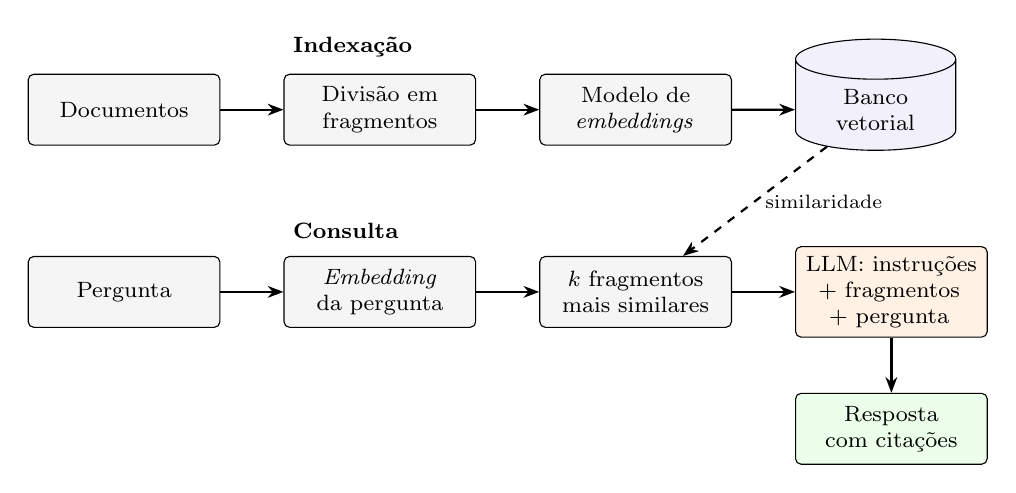
\begin{tikzpicture}[
  node distance=6mm and 8mm,
  box/.style={draw, rounded corners=2pt, align=center, font=\footnotesize, minimum height=9mm, text width=22mm, fill=gray!8},
  db/.style={draw, cylinder, shape border rotate=90, aspect=0.25, align=center, font=\footnotesize, minimum height=11mm, text width=18mm, fill=blue!6},
  arr/.style={-{Stealth[length=2mm]}, thick},
  lab/.style={font=\footnotesize\bfseries}
]
\node[box] (docs) {Documentos};
\node[box, right=of docs] (chunk) {Divisão em fragmentos};
\node[box, right=of chunk] (emb) {Modelo de \textit{embeddings}};
\node[db, right=of emb] (vdb) {Banco vetorial};
\draw[arr] (docs) -- (chunk); \draw[arr] (chunk) -- (emb); \draw[arr] (emb) -- (vdb);
\node[box, below=14mm of docs] (q) {Pergunta};
\node[box, right=of q] (qemb) {\textit{Embedding} da pergunta};
\node[box, right=of qemb] (topk) {$k$ fragmentos mais similares};
\node[box, right=of topk, fill=orange!10] (llm) {LLM: instruções + fragmentos + pergunta};
\node[box, below=7mm of llm, fill=green!8] (resp) {Resposta com citações};
\draw[arr] (q) -- (qemb); \draw[arr] (qemb) -- (topk); \draw[arr] (topk) -- (llm); \draw[arr] (llm) -- (resp);
\draw[arr, dashed] (vdb) -- node[right, font=\scriptsize]{similaridade} (topk);
\node[lab, above=1mm of chunk.north west, anchor=south west] {Indexação};
\node[lab, above=1mm of qemb.north west, anchor=south west] {Consulta};
\end{tikzpicture}
\caption{Funcionamento do RAG vetorial tradicional.}
\label{fig-rag-vetorial}
\end{figure}

Diversas variações procuram melhorar a recuperação. Uma delas, relevante para este trabalho por ser usada na busca DRIFT do GraphRAG, é a técnica HyDE (\textit{Hypothetical Document Embeddings}) \cite{gao2023hyde}: em vez de buscar com o \textit{embedding} da pergunta, o modelo primeiro escreve uma resposta hipotética, e o \textit{embedding} dessa resposta é usado na busca, por estar mais próximo, em forma e vocabulário, dos documentos procurados.

Apesar de eficaz em muitos cenários, o RAG vetorial apresenta limitações relevantes para este trabalho:

\begin{itemize}
    \item \textbf{Fragmentos isolados.} A recuperação considera cada fragmento separadamente, sem representar as relações entre partes do corpus. Perguntas que exigem conectar vários trechos (raciocínio em múltiplos saltos, ou \textit{multi-hop}) dependem de que todos esses trechos sejam, individualmente, similares à pergunta.
    \item \textbf{Perguntas globais.} Perguntas sobre o corpus como um todo -- ``quais são os principais temas?'', ``quais são os direitos do consumidor?'' -- exigiriam sintetizar informação dispersa por muitos fragmentos, o que não cabe em um pequeno conjunto recuperado. \citeonline{edge2024global} caracterizam essas perguntas como tarefas de sumarização focada na consulta (\textit{query-focused summarization}), para as quais o RAG vetorial não é adequado.
    \item \textbf{Similaridade não é relevância.} Fragmentos que compartilham o vocabulário da pergunta podem ser recuperados à frente do trecho que efetivamente responde a ela. No domínio jurídico, em que muitos artigos usam os mesmos termos (``consumidor'', ``fornecedor'', ``produto''), esse efeito é acentuado.
\end{itemize}

%%% Início de seção. %%%
\section{Grafos de Conhecimento}
\label{sec-referencial-kg}

Um grafo de conhecimento representa conhecimento como um grafo cujos nós são entidades do domínio e cujas arestas são relações entre elas \cite{hogan2021knowledge}. Na variante de grafo de propriedades, nós e arestas podem carregar atributos -- tipo, descrição, peso. Grafos de conhecimento permitem consultas que percorrem relações (``quais obrigações decorrem deste artigo, e quais sanções se aplicam ao seu descumprimento?'') e oferecem uma representação explícita e inspecionável do conteúdo do corpus.

Tradicionalmente, a construção de grafos de conhecimento a partir de texto exigia sistemas de extração de informação treinados para cada domínio. LLMs tornaram possível extrair entidades e relações a partir de instruções e de poucos exemplos, o que aproximou as duas áreas: grafos podem complementar LLMs com conhecimento estruturado e verificável, e LLMs podem construir e consultar grafos \cite{pan2024unifying}. O custo dessa abordagem é que a qualidade do grafo depende da qualidade da extração feita pelo modelo -- que pode omitir entidades, criar entidades duplicadas com nomes diferentes ou relações sem fundamento no texto -- e que cada fragmento do corpus exige ao menos uma chamada ao modelo.

%%% Início de seção. %%%
\section{Detecção de Comunidades}
\label{sec-referencial-comunidades}

Em grafos reais, é comum que os nós se organizem em grupos densamente conectados internamente e esparsamente conectados entre si, chamados comunidades \cite{fortunato2010community}. A detecção de comunidades busca particionar o grafo nesses grupos. Uma medida clássica da qualidade de uma partição é a modularidade \cite{newman2006modularity}, que compara a fração de arestas internas às comunidades com a fração esperada em um grafo aleatório com os mesmos graus:

\begin{equation}
\label{eq-modularidade}
Q = \frac{1}{2m} \sum_{i,j} \left[ A_{ij} - \frac{k_i k_j}{2m} \right] \delta(c_i, c_j)
\end{equation}

\noindent em que $A$ é a matriz de adjacência, $k_i$ é o grau do nó $i$, $m$ é o número de arestas e $\delta(c_i, c_j)$ vale 1 se os nós $i$ e $j$ estão na mesma comunidade.

O algoritmo de Louvain \cite{blondel2008fast} otimiza a modularidade de forma gulosa e hierárquica: move nós entre comunidades enquanto houver ganho e, em seguida, agrega cada comunidade em um único nó e repete o processo. O algoritmo de Leiden \cite{traag2019louvain} corrige um defeito do Louvain, que pode produzir comunidades mal conectadas ou até desconexas, com uma etapa de refinamento que garante comunidades bem conectadas. O GraphRAG utiliza uma versão hierárquica do Leiden: comunidades maiores que um tamanho máximo são novamente particionadas, formando uma hierarquia em que o nível 0 contém poucas comunidades amplas e os níveis seguintes, comunidades progressivamente menores e mais específicas.

%%% Início de seção. %%%
\section{RAG Baseado em Grafos}
\label{sec-referencial-graphrag}

O RAG baseado em grafos (\textit{Graph RAG}) reúne abordagens que utilizam grafos na recuperação: o conhecimento é organizado como grafo, e a recuperação seleciona nós, arestas, caminhos ou subgrafos relevantes para a pergunta, que são convertidos em texto e inseridos no \textit{prompt} \cite{peng2024graph}. Em relação ao RAG vetorial, essas abordagens preservam explicitamente a estrutura relacional do corpus, permitem percorrer relações em múltiplos saltos e possibilitam resumos sobre grupos de entidades.

O GraphRAG da Microsoft \cite{edge2024global} é uma dessas abordagens, voltada especificamente para corpora de texto não estruturado. Seu processo pode ser resumido em quatro passos: (i) um LLM extrai entidades e relações de cada fragmento do corpus, formando um grafo de conhecimento; (ii) o grafo é particionado em uma hierarquia de comunidades com o algoritmo de Leiden; (iii) o LLM gera, para cada comunidade, um relatório que resume suas entidades, relações e temas; e (iv) as consultas utilizam essas estruturas. Para perguntas globais, cada relatório de comunidade gera uma resposta parcial, e as respostas parciais são combinadas em uma resposta final (\textit{map-reduce}). Os autores mostraram que essa abordagem produz respostas mais abrangentes e diversas que o RAG vetorial para perguntas globais sobre corpora da ordem de um milhão de \textit{tokens}, com avaliação feita por um LLM em comparações par a par. A biblioteca evoluiu depois do artigo, incorporando a busca local (centrada em entidades) e a busca DRIFT \cite{microsoft2024drift}, que combina as buscas global e local. O \textit{framework} é descrito em detalhes no Capítulo~\ref{sec-graphrag}.

%%% Início de seção. %%%
\section{O Domínio Jurídico e o Código de Defesa do Consumidor}
\label{sec-referencial-juridico}

\subsection{Estrutura dos textos legislativos}
\label{sec-referencial-juridico-estrutura}

A elaboração e a redação das leis brasileiras seguem a Lei Complementar nº 95/1998 \cite{brasil1998lc95}, que define a estrutura dos textos legislativos. A unidade básica é o artigo, que pode se desdobrar em parágrafos, incisos, alíneas e itens. Os artigos podem ser agrupados em seções e subseções; estas, em capítulos; capítulos, em títulos; títulos, em livros; e livros, em partes. A mesma lei define regras de numeração: os artigos são numerados com ordinal até o nono (``Art. 9º'') e com cardinal a partir do décimo (``Art. 10.''). Artigos acrescentados por leis posteriores entre dois artigos existentes recebem o número do anterior seguido de letra maiúscula (``Art. 54-A''), sem renumeração dos demais. Dispositivos vetados pelo Presidente da República ou revogados por lei posterior permanecem no texto compilado com as indicações ``(Vetado)'' ou ``(Revogado)''.

Essa estrutura tem duas consequências importantes para o processamento automático. A primeira é que ela é regular o suficiente para ser reconhecida por expressões regulares, permitindo extrair cada artigo com a sua localização na hierarquia. A segunda é que a hierarquia carrega significado: um artigo localizado no capítulo ``Das Práticas Abusivas'' trata de práticas abusivas mesmo que o termo não apareça em seu texto. Preservar essa informação ao dividir o texto em fragmentos é, portanto, relevante para a qualidade da recuperação e da extração.

\subsection{O Código de Defesa do Consumidor}
\label{sec-referencial-juridico-cdc}

O Código de Defesa do Consumidor (Lei nº 8.078, de 11 de setembro de 1990) \cite{brasil1990cdc} estabelece normas de proteção e defesa do consumidor, de ordem pública e interesse social. O texto compilado utilizado neste trabalho tem 130 artigos -- os 119 artigos originais e 11 artigos acrescentados posteriormente, identificados por letras (42-A, 54-A a 54-G e 104-A a 104-C) --, organizados em seis títulos:

\begin{itemize}
    \item \textbf{Título I -- Dos Direitos do Consumidor} (arts. 1º a 60): disposições gerais e conceitos de consumidor, fornecedor, produto e serviço; política nacional das relações de consumo; direitos básicos (art. 6º); qualidade de produtos e serviços, responsabilidade pelo fato e pelo vício, decadência e prescrição; práticas comerciais (oferta, publicidade, práticas abusivas, cobrança de dívidas, bancos de dados); proteção contratual (cláusulas abusivas, contratos de adesão); prevenção e tratamento do superendividamento (arts. 54-A a 54-G, incluídos pela Lei nº 14.181/2021 \cite{brasil2021lei14181}); e sanções administrativas;
    \item \textbf{Título II -- Das Infrações Penais} (arts. 61 a 80): crimes contra as relações de consumo;
    \item \textbf{Título III -- Da Defesa do Consumidor em Juízo} (arts. 81 a 104-C): ações coletivas, coisa julgada e conciliação no superendividamento;
    \item \textbf{Título IV -- Do Sistema Nacional de Defesa do Consumidor} (arts. 105 e 106);
    \item \textbf{Título V -- Da Convenção Coletiva de Consumo} (arts. 107 e 108);
    \item \textbf{Título VI -- Disposições Finais} (arts. 109 a 119).
\end{itemize}

O CDC é um exemplo típico de texto de alta densidade relacional: os conceitos definidos nos primeiros artigos são usados em todo o código; direitos do Título I correspondem a obrigações do fornecedor, a sanções administrativas e a crimes do Título II; e a tutela coletiva do Título III remete a outras leis, como a Lei da Ação Civil Pública. O texto também contém doze artigos inteiramente vetados e diversos parágrafos e incisos vetados dentro de artigos vigentes.

\subsection{Processamento de linguagem natural no domínio jurídico}
\label{sec-referencial-juridico-pln}

O domínio jurídico tem vocabulário e estilo próprios, o que motivou modelos de linguagem especializados, como o LEGAL-BERT \cite{chalkidis2020legal}, e sistemas que combinam LLMs a bases de conhecimento jurídicas, como o ChatLaw \cite{cui2023chatlaw}. Com os LLMs de uso geral, o RAG tornou-se a abordagem predominante para assistentes jurídicos, por permitir fundamentar as respostas em legislação e jurisprudência atualizadas. A avaliação de ferramentas comerciais desse tipo mostrou, contudo, que a recuperação de trechos relevantes não garante respostas corretas: as ferramentas avaliadas ainda produziam afirmações incorretas ou com citações que não as sustentavam \cite{magesh2024hallucination}. Esses resultados motivam investigar estratégias de recuperação que representem melhor a estrutura relacional do direito, como a proposta neste trabalho.

%%% Início de seção. %%%
\section{Tecnologias Utilizadas}
\label{sec-referencial-tecnologias}

Como o foco do trabalho é a investigação do GraphRAG, as tecnologias de apoio foram escolhidas priorizando a integração direta com a biblioteca, a simplicidade e a reprodutibilidade. Esta seção apresenta brevemente cada uma; a forma como foram utilizadas é descrita nos capítulos~\ref{sec-indexacao} e~\ref{sec-aplicacao}.

\subsection{Biblioteca GraphRAG e componentes de dados}
\label{sec-referencial-tecnologias-graphrag}

\begin{itemize}
    \item \textbf{GraphRAG} \cite{graphraggithub, graphragdocs}: biblioteca Python de código aberto (licença MIT) que implementa a indexação e as consultas descritas no Capítulo~\ref{sec-graphrag}. É utilizada pela linha de comando (\textit{Command Line Interface} -- CLI), para indexar e ajustar \textit{prompts}, e como biblioteca, pelo \textit{backend} da aplicação. Este trabalho utiliza a versão 3.1.0, fixada em todos os ambientes.
    \item \textbf{LiteLLM} \cite{litellm}: biblioteca que oferece uma interface única para APIs de diversos provedores de modelos (OpenAI, Anthropic, Google, Ollama, entre outros). O GraphRAG a utiliza para todas as chamadas a modelos, o que permite trocar de provedor alterando apenas a configuração.
    \item \textbf{Apache Parquet} \cite{parquet}: formato de arquivo colunar em que o GraphRAG grava as tabelas produzidas pela indexação (documentos, fragmentos, entidades, relações, comunidades e relatórios).
    \item \textbf{LanceDB} \cite{lancedb}: banco vetorial embarcado em que o GraphRAG armazena os \textit{embeddings}.
    \item \textbf{Modelos da OpenAI} \cite{openaidocs}: modelos de linguagem e de \textit{embeddings} acessados por API, escolhidos por etapa conforme descrito na Seção~\ref{sec-indexacao-modelos}.
    \item \textbf{Ollama} \cite{ollama}: ferramenta para executar modelos de código aberto localmente, utilizada na primeira versão do projeto e mantida como configuração alternativa.
\end{itemize}

\subsection{\textit{Backend}}
\label{sec-referencial-tecnologias-backend}

\begin{itemize}
    \item \textbf{Python} e \textbf{FastAPI} \cite{fastapi}: o \textit{backend} é escrito em Python por ser a linguagem do GraphRAG, o que permite usar a biblioteca diretamente, sem intermediários. O FastAPI é um \textit{framework} web assíncrono, adequado a operações demoradas de entrada e saída como chamadas a modelos, e gera automaticamente a documentação da API.
    \item \textbf{REST} \cite{fielding2000rest}: estilo arquitetural adotado na API, em que recursos (consultas, histórico, grafo) são acessados por URLs e métodos HTTP.
    \item \textbf{\textit{Server-Sent Events}} (SSE) \cite{whatwgsse}: padrão da web para que o servidor envie uma sequência de eventos ao navegador em uma única conexão HTTP. É utilizado para transmitir, à medida que acontecem, as etapas de cada consulta.
    \item \textbf{SQLite} \cite{sqlite} e \textbf{SQLAlchemy} \cite{sqlalchemy}: o SQLite é um banco de dados relacional embarcado, armazenado em um único arquivo, sem servidor; o SQLAlchemy é a biblioteca de mapeamento objeto-relacional (ORM) utilizada para definir as tabelas e acessá-las a partir do Python.
\end{itemize}

\subsection{\textit{Frontend}}
\label{sec-referencial-tecnologias-frontend}

\begin{itemize}
    \item \textbf{React} \cite{react} e \textbf{TypeScript}: o \textit{frontend} é uma aplicação de página única (\textit{Single Page Application} -- SPA) construída com React, biblioteca de componentes de interface, e escrita em TypeScript, que acrescenta tipagem estática ao JavaScript.
    \item \textbf{Vite} \cite{vite}: ferramenta de desenvolvimento e empacotamento. Além de servir a aplicação, seu servidor de desenvolvimento atua como \textit{proxy} para a API, como descrito no Capítulo~\ref{sec-aplicacao}.
    \item \textbf{Tailwind CSS} \cite{tailwind} e componentes no estilo \textbf{shadcn/ui}: estilização por classes utilitárias e componentes de interface reutilizáveis.
    \item \textbf{react-force-graph} \cite{forcegraph}: componente de visualização de grafos com leiaute por simulação de forças, desenhado em \textit{canvas}, capaz de exibir os mais de mil nós e seis mil arestas do grafo do CDC com interação (zoom, arraste, seleção).
\end{itemize}

\subsection{Infraestrutura}
\label{sec-referencial-tecnologias-infra}

\begin{itemize}
    \item \textbf{Docker} e \textbf{Docker Compose} \cite{docker}: cada componente (ambiente de indexação, \textit{backend}, \textit{frontend} e, opcionalmente, o servidor de modelos locais) é executado em um contêiner, com dependências e versões definidas em arquivos de imagem. O Docker Compose descreve e orquestra os serviços em um único arquivo, o que garante que o sistema seja executado da mesma forma em qualquer máquina.
    \item \textbf{Git} e \textbf{GitHub}: controle de versão do código, da configuração e dos \textit{prompts}, e publicação do índice gerado como versão (\textit{release}) do repositório.
\end{itemize}

% ==============================================================================
% Monografia - Áurea Santos de Oliveira
% Capítulo 3 - O framework GraphRAG
% ==============================================================================
\chapter{O \textit{Framework} GraphRAG}
\label{sec-graphrag}

Este capítulo descreve em detalhes o GraphRAG na versão 3.1.0, utilizada neste trabalho. Além da documentação oficial \cite{graphragdocs}, a descrição baseia-se na leitura do código-fonte da biblioteca \cite{graphraggithub}, necessária porque parte do comportamento relevante -- como a divisão do contexto entre tipos de registro ou a forma como a busca DRIFT escolhe as perguntas que aprofunda -- não está documentada. A Seção~\ref{sec-graphrag-visao} apresenta a organização da biblioteca. As seções~\ref{sec-graphrag-indexacao} e~\ref{sec-graphrag-dados} descrevem o \textit{pipeline} de indexação e os dados que ele produz. A Seção~\ref{sec-graphrag-consultas} detalha as quatro modalidades de consulta. A Seção~\ref{sec-graphrag-prompts} trata dos \textit{prompts} e do ajuste automático de \textit{prompts}. A Seção~\ref{sec-graphrag-config} apresenta as opções de configuração e seus efeitos em qualidade e custo, e a Seção~\ref{sec-graphrag-defeitos} resume os defeitos e comportamentos não documentados identificados durante o trabalho.

%%% Início de seção. %%%
\section{Visão Geral e Organização}
\label{sec-graphrag-visao}

O GraphRAG é distribuído como pacote Python sob licença MIT. A partir da versão 3, sua estrutura foi reorganizada em pacotes menores. O pacote principal, \code{graphrag}, reúne o \textit{pipeline} de indexação, os motores de consulta, o ajuste de \textit{prompts}, a API e a CLI; os demais tratam de acesso a modelos (por meio do LiteLLM \cite{litellm}), segmentação de texto, leitura da entrada, armazenamento, cache e bancos vetoriais.

O uso mais comum é pela linha de comando, que oferece os comandos:

\begin{itemize}
    \item \code{graphrag init}: cria a estrutura de um projeto, com um \code{settings.yaml}, um arquivo \code{.env} para as chaves de API e os \textit{prompts} padrão;
    \item \code{graphrag index}: executa o \textit{pipeline} de indexação;
    \item \code{graphrag update}: atualiza um índice existente com novos documentos, sem reprocessar os anteriores;
    \item \code{graphrag prompt-tune}: gera \textit{prompts} de indexação adaptados ao corpus (Seção~\ref{sec-graphrag-prompts-tune});
    \item \code{graphrag query}: executa uma consulta em uma das modalidades (\code{--method local}, \code{global}, \code{drift} ou \code{basic}).
\end{itemize}

Um projeto do GraphRAG é uma pasta raiz (passada com a opção \code{--root}) com a estrutura padrão mostrada na Listagem~\ref{lst-estrutura-raiz}. Toda a configuração fica no \code{settings.yaml}; os \textit{prompts} ficam em arquivos de texto referenciados pela configuração; e todo o resultado da indexação fica na pasta \code{output}. As mesmas funções da CLI estão disponíveis como API Python (\code{graphrag.api}), e os motores de consulta podem ser montados diretamente a partir de suas classes, como faz o \textit{backend} deste trabalho (Capítulo~\ref{sec-aplicacao}).

\begin{lstlisting}[caption={Estrutura da pasta raiz de um projeto GraphRAG (a pasta \code{data/} deste trabalho).}, label=lst-estrutura-raiz]
data/
  settings.yaml        configuração completa (modelos, indexação e consultas)
  .env                 chaves de API 
  prompts/             prompts de indexação e de consulta (arquivos .txt)
  input/               documentos de entrada (texto, CSV ou JSON)
  output/              resultado da indexação: tabelas .parquet e banco vetorial LanceDB
  cache/               respostas dos modelos, reaproveitadas em novas execuções
  logs/                registros de execução
\end{lstlisting}

%%% Início de seção. %%%
\section{\textit{Pipeline} de Indexação}
\label{sec-graphrag-indexacao}

A indexação é organizada como uma sequência de \textit{workflows}, cada um responsável por uma etapa, que leem e gravam tabelas no armazenamento de saída. A biblioteca oferece três sequências pré-definidas: o método \textbf{padrão} (\textit{standard}), em que o grafo é extraído por um LLM; o método \textbf{rápido} (\textit{fast}), em que entidades são substituídas por sintagmas nominais extraídos com ferramentas tradicionais de PLN e as relações, por coocorrência; e o método de \textbf{atualização} (\textit{update}), que incorpora novos documentos a um índice existente. A sequência de \textit{workflows} pode ainda ser definida manualmente na configuração. Este trabalho utiliza o método padrão, cujas etapas são mostradas na Figura~\ref{fig-pipeline-indexacao} e descritas a seguir.

\begin{figure}[htb]
\centering
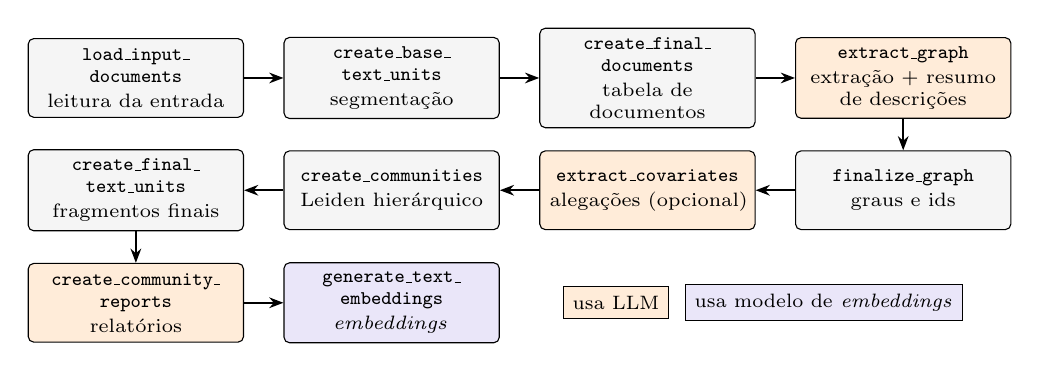
\begin{tikzpicture}[
  node distance=4mm and 5mm,
  wf/.style={draw, rounded corners=2pt, align=center, font=\scriptsize, minimum height=10mm, text width=25mm, fill=gray!8},
  llm/.style={wf, fill=orange!15},
  emb/.style={wf, fill=blue!10},
  arr/.style={-{Stealth[length=1.8mm]}, thick}
]
\node[wf] (a) {\code{load\_input\_documents}\\[1pt] leitura da entrada};
\node[wf, right=of a] (b) {\code{create\_base\_text\_units}\\[1pt] segmentação};
\node[wf, right=of b] (c) {\code{create\_final\_documents}\\[1pt] tabela de documentos};
\node[llm, right=of c] (d) {\code{extract\_graph}\\[1pt] extração + resumo de descrições};
\node[wf, below=of d] (e) {\code{finalize\_graph}\\[1pt] graus e ids};
\node[llm, left=of e] (f) {\code{extract\_covariates}\\[1pt] alegações (opcional)};
\node[wf, left=of f] (g) {\code{create\_communities}\\[1pt] Leiden hierárquico};
\node[wf, left=of g] (h) {\code{create\_final\_text\_units}\\[1pt] fragmentos finais};
\node[llm, below=of h] (i) {\code{create\_community\_reports}\\[1pt] relatórios};
\node[emb, right=of i] (j) {\code{generate\_text\_embeddings}\\[1pt] \textit{embeddings}};
\draw[arr] (a)--(b); \draw[arr] (b)--(c); \draw[arr] (c)--(d); \draw[arr] (d)--(e); \draw[arr] (e)--(f); \draw[arr] (f)--(g); \draw[arr] (g)--(h); \draw[arr] (h)--(i); \draw[arr] (i)--(j);
\node[draw, fill=orange!15, font=\scriptsize, right=8mm of j] (l1) {usa LLM};
\node[draw, fill=blue!10, font=\scriptsize, right=2mm of l1] (l2) {usa modelo de \textit{embeddings}};
\end{tikzpicture}
\caption{\textit{Workflows} do método padrão de indexação do GraphRAG 3.1.0.}
\label{fig-pipeline-indexacao}
\end{figure}

\subsection{Leitura e segmentação do texto}
\label{sec-graphrag-indexacao-segmentacao}

Os documentos de entrada podem ser arquivos de texto, CSV ou JSON. Nos formatos estruturados, a configuração indica qual campo contém o identificador, o título e o texto de cada documento; os demais campos ficam disponíveis como metadados. Cada documento é então dividido em unidades de texto (\textit{text units}) de tamanho fixo em \textit{tokens} (padrão: 1.200), com sobreposição entre unidades consecutivas (padrão: 100). Opcionalmente, campos de metadados do documento podem ser inseridos no início de cada unidade (\code{prepend\_metadata}), de modo que o modelo veja, junto com o trecho, informações como a sua localização no documento. As unidades de texto são a granularidade de todo o processamento seguinte: cada uma é enviada separadamente ao modelo na extração, e é a elas que as entidades e relações extraídas ficam vinculadas.

\subsection{Extração do grafo}
\label{sec-graphrag-indexacao-extracao}

Na etapa \code{extract\_graph}, cada unidade de texto é inserida no \textit{prompt} de extração, que contém instruções, a lista de tipos de entidade permitidos, exemplos de extração e o texto a processar. O modelo responde em um formato textual delimitado: cada entidade é emitida com nome, tipo e descrição, e cada relação, com entidade de origem, entidade de destino, descrição e uma força de 1 a 10 (a Listagem~\ref{lst-formato-extracao} mostra o formato com um exemplo real deste trabalho).

\begin{lstlisting}[caption={Formato de saída da extração de entidades e relações (exemplo simplificado).}, label=lst-formato-extracao]
("entity"<|>ART. 49 DO CDC<|>dispositivo_legal<|>Dispositivo vigente ... Assegura ao consumidor
   o direito de desistir do contrato celebrado fora do estabelecimento comercial em sete dias ...)
##
("entity"<|>DIREITO DE ARREPENDIMENTO<|>direito<|>Permite ao consumidor desistir ...)
##
("relationship"<|>CONSUMIDOR<|>DIREITO DE ARREPENDIMENTO<|>O consumidor é titular do direito de
   arrependimento previsto no art. 49 ...<|>9)
##
<|COMPLETE|>
\end{lstlisting}

Para aumentar a cobertura, a extração pode ser repetida sobre a mesma unidade de texto em rodadas adicionais (\textit{gleanings}), controladas por \code{max\_gleanings}. Em cada rodada, a conversa continua com a mensagem fixa ``MANY entities and relationships were missed in the last extraction'' e o modelo acrescenta entidades e relações. Entre rodadas, o modelo é perguntado se ainda há entidades faltando (resposta ``Y'' ou ``N''), o que pode encerrar o processo antes do limite. Com \code{max\_gleanings} igual a 1, cada unidade de texto custa duas chamadas ao modelo.

Concluída a extração, os resultados de todas as unidades são combinados. Entidades com o mesmo nome \textbf{e} o mesmo tipo são fundidas em uma única entidade, que acumula a lista de descrições parciais e a lista de unidades de texto em que aparece (sua frequência). Relações com a mesma origem e o mesmo destino também são fundidas, e o peso resultante é a soma das forças atribuídas em cada ocorrência, como detalhado a seguir. Esse critério de fusão tem duas consequências práticas: nomes diferentes para a mesma entidade geram nós duplicados, e o mesmo nome com tipos diferentes também gera nós distintos. Relações que citam entidades não extraídas são descartadas. Por isso, a padronização de nomes no \textit{prompt} de extração tem efeito direto sobre a qualidade do grafo.

\subsubsection*{Peso das relações}

O peso de uma relação é calculado em dois passos. Na extração, o \textit{prompt} pede ao modelo que atribua a cada relação uma força (\textit{relationship strength}), um número inteiro de 1 a 10 que indica a intensidade da ligação entre as duas entidades; é o último campo de cada relação na Listagem~\ref{lst-formato-extracao}. Se esse campo não puder ser lido como número, a biblioteca atribui o valor 1. Na fusão, todas as ocorrências de um mesmo par origem--destino -- em diferentes unidades de texto e nas rodadas adicionais de extração -- são reunidas, e o peso final é a \textbf{soma} das forças:

\begin{equation}
\label{eq-peso}
w(a, b) = \sum_{o \in O(a,b)} f_o
\end{equation}

\noindent em que $O(a,b)$ é o conjunto de ocorrências da relação de $a$ para $b$ e $f_o \in \{1, \dots, 10\}$ é a força atribuída pelo modelo em cada ocorrência. O peso combina, portanto, a intensidade atribuída pelo modelo e a frequência com que a relação aparece no corpus. No índice deste trabalho, o segundo fator domina: o modelo atribuiu força 10 à grande maioria das relações (5.773 das 6.885 têm peso exatamente 10), e 97\% delas aparecem em uma única unidade de texto, de modo que o peso se aproxima de dez vezes o número de artigos em que a relação é mencionada. Os maiores pesos são os das relações entre CONSUMIDOR e DIREITO À INFORMAÇÃO (243, em 26 artigos) e entre FORNECEDOR e PRODUTO (219, em 22 artigos).

O peso é usado em dois pontos. Na detecção de comunidades, o grafo é tratado como não direcionado e o peso de cada aresta é passado ao algoritmo de Leiden, de modo que relações frequentes aproximam as entidades na mesma comunidade; quando existem as duas direções de um mesmo par, apenas uma é mantida, sem somar os pesos. Na busca local, o peso é incluído como coluna na tabela de relações enviada ao modelo, mas a ordenação das relações que entram no contexto usa outro atributo, o grau combinado (\code{combined\_degree}), que é a soma dos graus das duas entidades da relação.

\subsection{Resumo de descrições}
\label{sec-graphrag-indexacao-resumo}

Uma entidade que aparece em várias unidades de texto acumula várias descrições parciais. Na etapa de resumo (\code{summarize\_descriptions}), que é executada dentro do \textit{workflow} \code{extract\_graph}, o LLM funde essas descrições em uma única descrição coerente, limitada a um número máximo de palavras (\code{max\_length}). O mesmo é feito para as relações. Entidades e relações com uma única descrição não geram chamadas. Trata-se de uma tarefa simples de síntese, que pode ser atribuída a um modelo mais barato que o da extração.

\subsection{Alegações (\textit{claims})}
\label{sec-graphrag-indexacao-claims}

Opcionalmente, o \textit{workflow} \code{extract\_covariates} extrai alegações (\textit{claims}): afirmações factuais associadas a entidades, com status (verdadeira, falsa, suspeita) e período. A etapa foi concebida para corpora como notícias e investigações e vem desabilitada por padrão. Neste trabalho ela não foi utilizada, pois no texto de uma lei as ``afirmações'' são as próprias normas, já representadas pelas entidades de tipo direito, obrigação e afins.

\subsection{Detecção de comunidades}
\label{sec-graphrag-indexacao-comunidades}

O \textit{workflow} \code{finalize\_graph} calcula atributos do grafo, como o grau de cada nó. Em seguida, \code{create\_communities} aplica o algoritmo de Leiden hierárquico (Seção~\ref{sec-referencial-comunidades}) ao grafo de entidades, usando o peso das relações. Comunidades com mais entidades que \code{max\_cluster\_size} (padrão: 10) são subdivididas recursivamente, formando os níveis da hierarquia. Por padrão, considera-se apenas o maior componente conexo do grafo (\code{use\_lcc}), e uma semente fixa (\code{seed}) torna o particionamento determinístico.

\subsection{Relatórios de comunidade}
\label{sec-graphrag-indexacao-relatorios}

Para cada comunidade, de todos os níveis, o \textit{workflow} \code{create\_community\_reports} monta um contexto com as entidades e relações da comunidade -- e, nas comunidades de níveis superiores cujo conteúdo excede o limite \code{max\_input\_length}, com os relatórios das subcomunidades -- e pede ao LLM um relatório estruturado em JSON contendo: título, resumo, uma nota de importância de 0 a 10 com justificativa e uma lista de constatações (\textit{findings}), cada uma com resumo e explicação. As afirmações do relatório citam as entidades e relações em que se baseiam. O relatório completo, convertido em texto, é o que as buscas global e DRIFT utilizam. O tamanho máximo do relatório é controlado por \code{max\_length}. No método rápido, os relatórios são gerados a partir do texto original, com outro \textit{prompt}.

\subsection{\textit{Embeddings}}
\label{sec-graphrag-indexacao-embeddings}

Por fim, \code{generate\_text\_embeddings} gera, com o modelo de \textit{embeddings}, vetores para três conjuntos de textos e os armazena no banco vetorial: as descrições das entidades (usadas pela busca local para encontrar as entidades relacionadas à pergunta), o conteúdo completo dos relatórios de comunidade (usado pela busca DRIFT) e o texto das unidades de texto (usado pela busca básica).

\subsection{Cache}
\label{sec-graphrag-indexacao-cache}

Todas as respostas dos modelos são gravadas em cache, indexadas pelo conteúdo da requisição (\textit{prompt} e parâmetros). Se a indexação for executada novamente sem alteração de texto, \textit{prompt} ou configuração de uma etapa, as respostas são lidas do cache, sem custo. Na prática, isso permite reexecutar a indexação -- por exemplo, para alterar apenas a detecção de comunidades -- pagando apenas pelas etapas que mudaram. Também permite que uma indexação interrompida seja retomada sem refazer as chamadas já concluídas.

%%% Início de seção. %%%
\section{Dados Produzidos}
\label{sec-graphrag-dados}

O resultado da indexação é um conjunto de tabelas em formato Parquet e um banco vetorial LanceDB, resumidos na Tabela~\ref{tab-tabelas-saida}. Cada registro tem um identificador interno (UUID) e um identificador curto sequencial (\code{human\_readable\_id}); é o identificador curto que aparece no contexto enviado ao modelo nas consultas e, portanto, nas citações das respostas (por exemplo, ``\code{[Data: Sources (49)]}'').

\begin{table}[htb]
\centering
\caption{Tabelas produzidas pela indexação do GraphRAG 3.1.0.}
\label{tab-tabelas-saida}
\footnotesize
\begin{tabular}{L{3.6cm} L{10.6cm}}
\toprule
\textbf{Arquivo} & \textbf{Conteúdo e principais colunas} \\
\midrule
\code{documents.parquet} & Documentos de entrada: título, texto, metadados originais (\code{raw\_data}) e unidades de texto do documento. \\
\code{text\_units.parquet} & Unidades de texto: texto, número de \textit{tokens}, documento de origem e ids das entidades e relações extraídas dela. \\
\code{entities.parquet} & Entidades: nome (\code{title}), tipo, descrição resumida, unidades de texto de origem, frequência e grau. \\
\code{relationships.parquet} & Relações: origem, destino, descrição, peso, grau combinado das extremidades e unidades de texto de origem. \\
\code{communities.parquet} & Comunidades: nível, comunidade-mãe e filhas, entidades, relações e unidades de texto que contém e tamanho. \\
\code{community\_reports.parquet} & Relatórios: título, resumo, nota (\code{rank}) e sua justificativa, constatações, conteúdo completo em texto e JSON. \\
\code{covariates.parquet} & Alegações (apenas se \code{extract\_claims} estiver habilitado). \\
\code{lancedb/} & Banco vetorial com os \textit{embeddings} das descrições de entidades, dos relatórios e das unidades de texto. \\
\code{stats.json}, \code{context.json} & Estatísticas da execução (tempo por \textit{workflow}) e estado do \textit{pipeline}. \\
\bottomrule
\end{tabular}
\end{table}

%%% Início de seção. %%%
\section{Modalidades de Consulta}
\label{sec-graphrag-consultas}

O GraphRAG oferece quatro modalidades de consulta. Em todas, o resultado final é produzido por um LLM a partir de um \textit{prompt} que contém instruções, o contexto recuperado formatado como tabelas e a pergunta, e as instruções pedem que cada afirmação cite os registros que a sustentam no formato \code{[Data: <tabela> (<ids>)]}. As modalidades diferem no que é recuperado, em quantas chamadas ao modelo são feitas e, portanto, no custo. Dois parâmetros são comuns às consultas: o \textbf{nível de comunidade} (\code{community\_level}, padrão 2 na CLI), que determina até que nível da hierarquia os relatórios de comunidade são considerados, e o \textbf{tipo de resposta} (\code{response\_type}, padrão ``\textit{Multiple Paragraphs}''), que descreve ao modelo o formato desejado.

\subsection{Busca local}
\label{sec-graphrag-consultas-local}

A busca local é indicada para perguntas sobre entidades específicas. Seu ponto de partida é o grafo: a pergunta é convertida em \textit{embedding} e comparada às descrições das entidades, e as entidades mais similares (\code{top\_k\_entities}, padrão 10) são selecionadas. A partir delas, o contexto é expandido com as relações dessas entidades (até \code{top\_k\_relationships} por entidade, priorizando as que ligam entidades selecionadas entre si), os relatórios das comunidades a que pertencem e as unidades de texto de onde foram extraídas.

Todo esse material compete por um orçamento de contexto (\code{max\_context\_tokens}, padrão 12 mil \textit{tokens}), dividido em três partes por dois parâmetros: \code{text\_unit\_prop} (padrão 0,5) reserva uma fração para as unidades de texto, \code{community\_prop} (padrão 0,15) reserva outra para os relatórios de comunidade, e o restante (0,35) é preenchido com as tabelas de entidades e relações. Cada parte é preenchida em ordem de relevância até esgotar sua fração. O contexto resultante tem a forma de tabelas delimitadas, com os identificadores curtos que o modelo deve citar. A busca local faz uma única chamada ao modelo.

\subsection{Busca global}
\label{sec-graphrag-consultas-global}

A busca global é indicada para perguntas sobre o corpus como um todo e segue a estratégia \textit{map-reduce} do artigo original \cite{edge2024global}:

\begin{enumerate}
    \item são selecionados os relatórios de comunidade até o nível \code{community\_level};
    \item \textbf{map}: os relatórios são embaralhados e agrupados em lotes de até \code{max\_context\_tokens} \textit{tokens}; cada lote é enviado ao modelo em uma chamada separada, que devolve uma lista de pontos-chave relevantes para a pergunta, cada um com uma nota de importância de 0 a 100;
    \item \textbf{reduce}: os pontos-chave de todos os lotes com nota maior que zero são ordenados pela nota e, até o limite \code{data\_max\_tokens}, enviados a uma chamada final que redige a resposta.
\end{enumerate}

O número de chamadas é aproximadamente o número de lotes mais um, e cresce rapidamente com o nível de comunidade: níveis mais profundos têm mais comunidades e, portanto, mais relatórios. Como alternativa ao nível fixo, a seleção dinâmica de comunidades percorre a hierarquia a partir da raiz e pergunta ao modelo, para cada relatório visitado, se ele é relevante para a pergunta, descendo apenas pelos ramos relevantes; essa seleção faz chamadas adicionais de classificação.

\subsection{Busca DRIFT}
\label{sec-graphrag-consultas-drift}

A busca DRIFT (\textit{Dynamic Reasoning and Inference with Flexible Traversal}) \cite{microsoft2024drift} combina as buscas global e local de forma iterativa, conforme a Figura~\ref{fig-drift}. No código da versão 3.1.0, ela funciona da seguinte forma:

\begin{enumerate}
    \item \textbf{Expansão da pergunta}: o modelo escreve uma resposta hipotética à pergunta, usando como modelo de formato um relatório de comunidade sorteado. O \textit{embedding} dessa resposta é usado para a busca, segundo a técnica HyDE \cite{gao2023hyde} (1 chamada);
    \item \textbf{Seleção de relatórios}: os \code{drift\_k\_followups} relatórios (padrão 20) mais similares à resposta hipotética são selecionados;
    \item \textbf{Primer}: os relatórios selecionados são divididos em \code{primer\_folds} grupos (padrão 5), e cada grupo é enviado ao modelo, que devolve uma resposta parcial, uma nota e uma lista de perguntas de acompanhamento (\textit{follow-ups});
    \item \textbf{Aprofundamento}: em cada uma de \code{n\_depth} rodadas (padrão 3), até \code{drift\_k\_followups} perguntas ainda não respondidas são escolhidas, e cada uma é respondida por uma busca local completa, que também gera novas perguntas de acompanhamento;
    \item \textbf{Redução}: todas as respostas parciais são enviadas a uma chamada final, que redige a resposta.
\end{enumerate}

\begin{figure}[htb]
\centering
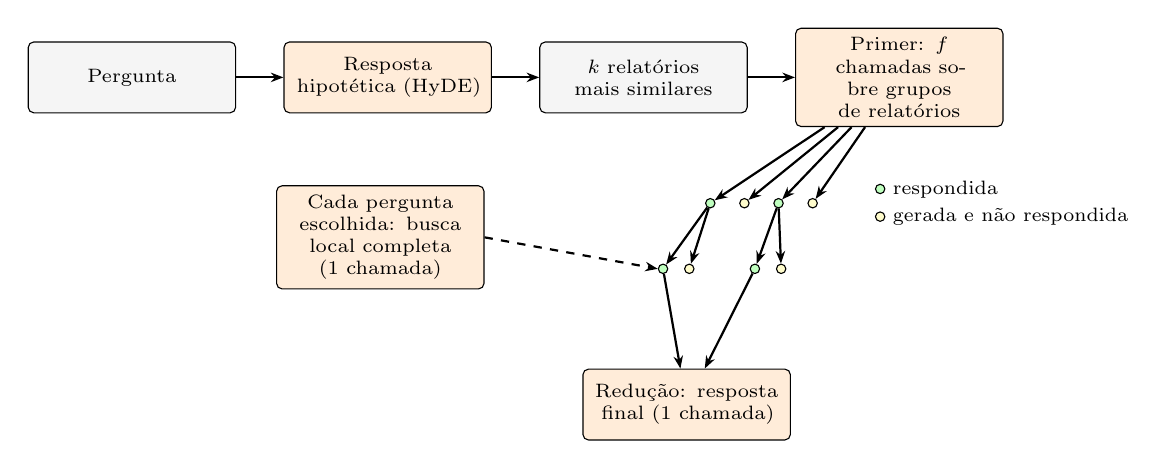
\begin{tikzpicture}[
  node distance=5mm and 6mm,
  box/.style={draw, rounded corners=2pt, align=center, font=\scriptsize, minimum height=9mm, text width=24mm, fill=gray!8},
  llm/.style={box, fill=orange!15},
  q/.style={draw, circle, inner sep=1.2pt, font=\tiny, fill=yellow!20},
  qa/.style={q, fill=green!25},
  arr/.style={-{Stealth[length=1.6mm]}, thick}
]
\node[box] (p) {Pergunta};
\node[llm, right=of p] (h) {Resposta hipotética (HyDE)};
\node[box, right=of h] (r) {$k$ relatórios mais similares};
\node[llm, right=of r] (pr) {Primer: $f$ chamadas sobre grupos de relatórios};
\draw[arr] (p)--(h); \draw[arr] (h)--(r); \draw[arr] (r)--(pr);
\node[qa, below=9mm of pr, xshift=-24mm] (q1) {}; \node[q, right=3mm of q1] (q2) {}; \node[qa, right=3mm of q2] (q3) {}; \node[q, right=3mm of q3] (q4) {};
\draw[arr] (pr) -- (q1); \draw[arr] (pr) -- (q2); \draw[arr] (pr) -- (q3); \draw[arr] (pr) -- (q4);
\node[qa, below=7mm of q1, xshift=-6mm] (q11) {}; \node[q, right=2mm of q11] (q12) {}; \node[qa, below=7mm of q3, xshift=-3mm] (q31) {}; \node[q, right=2mm of q31] (q32) {};
\draw[arr] (q1)--(q11); \draw[arr] (q1)--(q12); \draw[arr] (q3)--(q31); \draw[arr] (q3)--(q32);
\node[llm, left=22mm of q11, yshift=4mm] (loc) {Cada pergunta escolhida: busca local completa (1 chamada)};
\draw[arr, dashed] (loc.east) -- (q11.west);
\node[llm, below=12mm of q32, xshift=-12mm] (red) {Redução: resposta final (1 chamada)};
\draw[arr] (q31) -- (red); \draw[arr] (q11) -- (red);
\node[font=\scriptsize, align=left, right=6mm of q4] {\tikz\node[qa]{};~respondida\\[2pt]\tikz\node[q]{};~gerada e não respondida};
\end{tikzpicture}
\caption{Funcionamento da busca DRIFT no GraphRAG 3.1.0: a cada rodada, perguntas de acompanhamento são respondidas por buscas locais e geram novas perguntas.}
\label{fig-drift}
\end{figure}

A comparação entre o código da versão 3.1.0, a documentação oficial \cite{graphragdocs} e a publicação que apresentou a DRIFT \cite{microsoft2024drift} revelou comportamentos que não estão descritos, ou que estão descritos de forma diferente, e que são relevantes para a interpretação dos resultados:

\begin{itemize}
    \item \textbf{Seleção aleatória das perguntas.} A documentação descreve a saída como uma hierarquia de perguntas e respostas ordenadas por relevância, e a publicação menciona a confiança do algoritmo em continuar cada expansão. No código, porém, as perguntas aprofundadas em cada rodada são escolhidas \textbf{por sorteio} entre as não respondidas: a função que as ordena é chamada sem critério de pontuação e, nesse caso, embaralha a lista. As notas atribuídas pelo modelo às perguntas não são usadas para priorizá-las.
    \item \textbf{Modelo de formato sorteado na expansão.} A expansão da pergunta pela técnica HyDE é citada na publicação, mas não na documentação, e nenhuma das duas informa que a resposta hipotética é escrita no formato de um relatório de comunidade sorteado, outra fonte de variação entre execuções.
    \item \textbf{Duplo papel de \code{drift\_k\_followups}.} A documentação descreve a opção apenas como o número de resultados globais recuperados. No código, ela define também quantas perguntas são respondidas em cada rodada, sendo, por isso, o principal determinante do custo.
    \item \textbf{Proporções de contexto.} A documentação descreve \code{local\_search\_text\_unit\_prop} e \code{local\_search\_community\_prop} apenas como as proporções da busca dedicadas a trechos e a comunidades. Não informa que o restante é o espaço das entidades e relações, nem que, com os valores padrão (0,9 e 0,1), esse restante é zero.
    \item \textbf{Opções sem efeito.} As opções \code{primer\_llm\_max\_tokens}, \code{data\_max\_tokens}, \code{reduce\_max\_tokens} e \code{concurrency} estão documentadas, mas não são lidas pelo código da DRIFT.
    \item \textbf{Perguntas não respondidas na saída.} Como cada busca local gera novas perguntas, a árvore final contém muitas perguntas que foram geradas e nunca respondidas, o que é o funcionamento normal do algoritmo, mas não é mencionado.
\end{itemize}

Com os valores padrão, o número de chamadas é $1 + 5 + 3 \times 20 + 1 = 67$, valor confirmado em uma consulta real deste trabalho (Capítulo~\ref{sec-aplicacao}).

\subsection{Busca básica}
\label{sec-graphrag-consultas-basic}

A busca básica (\textit{basic search}) é uma implementação de RAG vetorial tradicional: a pergunta é convertida em \textit{embedding}, as $k$ unidades de texto mais similares (padrão 10) são recuperadas do banco vetorial e inseridas no \textit{prompt}, e o modelo gera a resposta em uma única chamada. Ela não utiliza entidades, relações ou comunidades. Por compartilhar com as demais modalidades o mesmo corpus, a mesma segmentação, o mesmo modelo de \textit{embeddings} e o mesmo modelo gerador, ela é usada neste trabalho como referência de RAG vetorial (\textit{baseline}): a diferença entre ela e as demais modalidades é, essencialmente, o uso da estrutura de grafo.

\subsection{Comparação entre as modalidades}
\label{sec-graphrag-consultas-comparacao}

A Tabela~\ref{tab-modalidades} resume as quatro modalidades.

\begin{table}[htb]
\centering
\caption{Comparação entre as modalidades de consulta do GraphRAG 3.1.0 (valores padrão).}
\label{tab-modalidades}
\footnotesize
\renewcommand{\arraystretch}{1.5}
\begin{tabular}{L{1.6cm} L{3.6cm} L{3.9cm} L{4.6cm}}
\toprule
\textbf{Modalidade} & \textbf{Ponto de partida} & \textbf{Contexto enviado ao modelo} & \textbf{Chamadas ao modelo} \\
\midrule
Básica & Unidades de texto similares à pergunta & 10 unidades de texto & 1 \\
\addlinespace[4pt]
Local & Entidades similares à pergunta & Entidades, relações, relatórios e unidades de texto (12 mil \textit{tokens}) & 1 \\
\addlinespace[4pt]
Global & Todos os relatórios até o nível escolhido & Lotes de relatórios (map); pontos-chave (reduce) & Número de lotes + 1; depende do nível \\
\addlinespace[4pt]
DRIFT & Relatórios similares a uma resposta hipotética & Relatórios (primer); contexto da busca local (cada pergunta); respostas parciais (redução) & $1 + f + d \times k + 1$ ($f$ grupos, $d$ rodadas, $k$ perguntas por rodada) \\
\bottomrule
\end{tabular}
\end{table}

%%% Início de seção. %%%
\section{\textit{Prompts}}
\label{sec-graphrag-prompts}

Todas as interações do GraphRAG com os modelos são guiadas por \textit{prompts} armazenados em arquivos de texto na pasta \code{prompts}, cujos caminhos são definidos no \code{settings.yaml}. Os \textit{prompts} contêm marcadores entre chaves (por exemplo, \code{\{input\_text\}} e \code{\{context\_data\}}) que a biblioteca substitui pelo conteúdo de cada chamada. A Tabela~\ref{tab-prompts} relaciona os \textit{prompts}, a etapa que os utiliza e os marcadores de cada um. Os \textit{prompts} de indexação determinam o que entra no grafo; alterá-los exige reindexar. Os de consulta determinam como as respostas são redigidas e podem ser alterados sem reindexação.

\begin{table}[htb]
\centering
\caption{\textit{Prompts} do GraphRAG 3.1.0.}
\label{tab-prompts}
\footnotesize
\begin{tabular}{L{5.6cm} L{4.4cm} L{4.2cm}}
\toprule
\textbf{Arquivo} & \textbf{Etapa} & \textbf{Marcadores} \\
\midrule
\multicolumn{3}{l}{\textit{Indexação}} \\
\code{extract\_graph.txt} & Extração de entidades e relações & \code{input\_text} \\
\code{summarize\_descriptions.txt} & Resumo de descrições & \code{entity\_name}, \code{description\_list} \\
\code{extract\_claims.txt} & Extração de alegações & \code{input\_text}, \code{entity\_specs}, \code{claim\_description} \\
\code{community\_report\_graph.txt} & Relatórios (método padrão) & \code{input\_text} \\
\code{community\_report\_text.txt} & Relatórios (método rápido) & \code{input\_text}, \code{max\_report\_length} \\
\midrule
\multicolumn{3}{l}{\textit{Consulta}} \\
\code{local\_search\_system\_prompt.txt} & Busca local & \code{context\_data}, \code{response\_type} \\
\code{global\_search\_map\_system\_prompt.txt} & Busca global (map) & \code{context\_data}, \code{max\_length} \\
\code{global\_search\_reduce\_system\_prompt.txt} & Busca global (reduce) & \code{report\_data}, \code{response\_type}, \code{max\_length} \\
\code{global\_search\_knowledge\_system\_prompt.txt} & Busca global (conhecimento geral) & -- \\
\code{drift\_search\_system\_prompt.txt} & DRIFT (buscas locais) & \code{context\_data}, \code{response\_type}, \code{global\_query}, \code{followups} \\
\code{drift\_reduce\_prompt.txt} & DRIFT (redução) & \code{context\_data}, \code{response\_type} \\
\code{basic\_search\_system\_prompt.txt} & Busca básica & \code{context\_data}, \code{response\_type} \\
\code{question\_gen\_system\_prompt.txt} & Geração de perguntas & \code{context\_data}, \code{question\_count} \\
\bottomrule
\end{tabular}
\end{table}

O \textit{prompt} de extração é o mais importante, por definir o grafo. Ele é organizado em seções: objetivo (``\textit{-Goal-}''), passos (``\textit{-Steps-}''), com a lista de tipos de entidade e o formato de saída; exemplos (``\textit{-Examples-}''), cada um com um texto de entrada e a extração esperada; e os dados reais (``\textit{-Real Data-}''), onde a unidade de texto é inserida. Os exemplos ensinam ao modelo, por demonstração, o nível de detalhe esperado, a forma de nomear entidades e o idioma das descrições. Como o \textit{prompt} é enviado em cada chamada de extração, seu tamanho multiplica o custo da indexação.

\subsection{Ajuste automático de \textit{prompts}}
\label{sec-graphrag-prompts-tune}

O comando \code{graphrag prompt-tune} gera \textit{prompts} de indexação adaptados ao corpus. Ele seleciona uma amostra de unidades de texto (por sorteio, pelas primeiras, por todas ou por similaridade) e, com o LLM: (i) identifica o domínio do corpus; (ii) cria uma \textit{persona} de especialista nesse domínio; (iii) descobre os tipos de entidade presentes, ou usa nenhum tipo pré-definido; (iv) gera exemplos de extração a partir das unidades amostradas; (v) define o papel do redator dos relatórios de comunidade e o critério da nota de importância; e (vi) monta os \textit{prompts} de extração, de resumo e de relatório, traduzindo as instruções de saída para o idioma do corpus. As limitações encontradas nesse comando, que levaram ao desenvolvimento de um \textit{script} próprio, são descritas na Seção~\ref{sec-graphrag-defeitos} e no Capítulo~\ref{sec-indexacao}.

%%% Início de seção. %%%
\section{Configuração}
\label{sec-graphrag-config}

O \code{settings.yaml} reúne toda a configuração do GraphRAG em seções. Antes de interpretar o arquivo, a biblioteca substitui referências a variáveis de ambiente no formato \verb|${NOME}| pelo valor correspondente, lido do arquivo \code{.env} da pasta raiz; é assim que as chaves de API são fornecidas sem que fiquem escritas na configuração. A configuração completa usada neste trabalho está no repositório do projeto (Seção~\ref{sec-indexacao-config}).

\subsection{Modelos}
\label{sec-graphrag-config-modelos}

As seções \code{completion\_models} e \code{embedding\_models} definem modelos nomeados, que são referenciados pelas demais seções por meio de identificadores (\code{completion\_model\_id} e \code{embedding\_model\_id}). Isso permite atribuir um modelo diferente a cada etapa da indexação e a cada modalidade de consulta. Para cada modelo, configuram-se: o provedor (\code{model\_provider}, repassado ao LiteLLM) e o nome do modelo; a autenticação (chave de API ou identidade gerenciada do Azure); o número de requisições simultâneas (\code{concurrent\_requests}) e o modo assíncrono; a política de novas tentativas em caso de erro (\code{max\_retries} e estratégia, como espera exponencial); limites de taxa; e os argumentos repassados a cada chamada (\code{call\_args}), como temperatura e tempo máximo de espera.

\subsection{Entrada, armazenamento e cache}
\label{sec-graphrag-config-armazenamento}

As seções \code{input}, \code{input\_storage}, \code{output\_storage}, \code{cache}, \code{reporting} e \code{vector\_store} definem o formato da entrada (texto, CSV ou JSON, e os campos de identificador, título e texto), onde ficam os arquivos de entrada e saída (sistema de arquivos local, Azure Blob Storage ou Cosmos DB), o cache, os registros e o banco vetorial (LanceDB, Azure AI Search ou Cosmos DB). A seção \code{snapshots} permite gravar artefatos intermediários adicionais, como o grafo em formato GraphML.

\subsection{Indexação}
\label{sec-graphrag-config-indexacao}

A Tabela~\ref{tab-config-indexacao} apresenta as principais opções das etapas de indexação, com seus valores padrão e seus efeitos.

\begin{longtable}{L{3.2cm} L{2.6cm} L{1.5cm} L{6.6cm}}
\caption{Principais opções de configuração da indexação.}
\label{tab-config-indexacao} \\
\toprule
\textbf{Seção} & \textbf{Opção} & \textbf{Padrão} & \textbf{Efeito} \\
\midrule
\endfirsthead
\multicolumn{4}{l}{\footnotesize\textit{(continuação)}} \\
\toprule
\textbf{Seção} & \textbf{Opção} & \textbf{Padrão} & \textbf{Efeito} \\
\midrule
\endhead
\bottomrule
\endfoot
\footnotesize \code{chunking} & \footnotesize \code{size}, \code{overlap} & \footnotesize 1200, 100 & \footnotesize Tamanho e sobreposição das unidades de texto. Unidades menores geram mais chamadas de extração e extrações mais detalhadas; maiores reduzem o custo e podem perder entidades. \\
 & \footnotesize \code{prepend\_metadata} & \footnotesize -- & \footnotesize Campos de metadados inseridos no início de cada unidade, dando ao modelo o contexto do documento. \\
 & \footnotesize \code{encoding\_model} & \footnotesize \code{o200k\_base} & \footnotesize Codificação usada para contar \textit{tokens}. \\
\midrule
\footnotesize \code{extract\_graph} & \footnotesize \code{entity\_types} & \footnotesize \textit{organization, person, geo, event} & \footnotesize Tipos de entidade inseridos no \textit{prompt} de extração. Definem a ontologia do grafo. \\
 & \footnotesize \code{max\_gleanings} & \footnotesize 1 & \footnotesize Rodadas adicionais de extração por unidade de texto. Cada rodada é uma chamada a mais por unidade. \\
 & \footnotesize \code{prompt}, modelo & \footnotesize -- & \footnotesize \textit{Prompt} e modelo da extração, a etapa que mais influencia a qualidade e o custo. \\
\midrule
\footnotesize \code{summarize\_descriptions} & \footnotesize \code{max\_length} & \footnotesize 500 & \footnotesize Tamanho máximo (em palavras) das descrições resumidas. \\
 & \footnotesize \code{max\_input\_tokens} & \footnotesize 4000 & \footnotesize Limite de descrições parciais por chamada de resumo. \\
\midrule
\footnotesize \code{cluster\_graph} & \footnotesize \code{max\_cluster\_size} & \footnotesize 10 & \footnotesize Tamanho máximo de uma comunidade antes de ser subdividida. Valores menores geram mais níveis e mais comunidades, portanto mais relatórios. \\
 & \footnotesize \code{use\_lcc}, \code{seed} & \footnotesize sim, fixo & \footnotesize Uso apenas do maior componente conexo; semente do algoritmo. \\
\midrule
\footnotesize \code{community\_reports} & \footnotesize \code{max\_length} & \footnotesize 2000 & \footnotesize Tamanho máximo dos relatórios. Relatórios maiores encarecem a indexação e todas as consultas global e DRIFT. \\
 & \footnotesize \code{max\_input\_length} & \footnotesize 8000 & \footnotesize Tamanho máximo do contexto de cada relatório. \\
\midrule
\footnotesize \code{extract\_claims} & \footnotesize \code{enabled} & \footnotesize não & \footnotesize Habilita a extração de alegações (mais uma chamada por unidade de texto). \\
\midrule
\footnotesize \code{extract\_graph\_nlp}, \code{prune\_graph} & \footnotesize diversas & \footnotesize -- & \footnotesize Extração por PLN tradicional e poda do grafo, usadas no método rápido. \\
\midrule
\footnotesize \code{embed\_text} & \footnotesize \code{names}, \code{batch\_size} & \footnotesize 3 conjuntos, 16 & \footnotesize Textos que recebem \textit{embeddings} e tamanho dos lotes enviados ao modelo. \\
\midrule
\footnotesize (raiz) & \footnotesize \code{workflows} & \footnotesize -- & \footnotesize Lista explícita de \textit{workflows}, substituindo a do método escolhido. \\
\end{longtable}

\subsection{Consultas}
\label{sec-graphrag-config-consultas}

As opções das modalidades de consulta estão nas seções \code{local\_search}, \code{global\_search}, \code{drift\_search} e \code{basic\_search}. Além do modelo e dos \textit{prompts}, elas controlam o tamanho do contexto e, nas modalidades com várias chamadas, quantas chamadas são feitas. A Tabela~\ref{tab-config-consultas} apresenta as opções e seus efeitos esperados em custo, com os valores medidos neste trabalho quando disponíveis.

\begin{longtable}{L{2.1cm} L{3.9cm} L{1.5cm} L{6.4cm}}
\caption{Opções de configuração das modalidades de consulta e seus efeitos.}
\label{tab-config-consultas} \\
\toprule
\textbf{Seção} & \textbf{Opção} & \textbf{Padrão} & \textbf{Efeito} \\
\midrule
\endfirsthead
\multicolumn{4}{l}{\footnotesize\textit{(continuação)}} \\
\toprule
\textbf{Seção} & \textbf{Opção} & \textbf{Padrão} & \textbf{Efeito} \\
\midrule
\endhead
\bottomrule
\endfoot
\footnotesize \code{basic\_search} & \footnotesize \code{k} & \footnotesize 10 & \footnotesize Número de unidades de texto recuperadas. Mais unidades aumentam a cobertura e os \textit{tokens} de entrada. \\
 & \footnotesize \code{max\_context\_tokens} & \footnotesize 12000 & \footnotesize Teto do contexto. \\
\midrule
\footnotesize \code{local\_search} & \footnotesize \code{top\_k\_entities} & \footnotesize 10 & \footnotesize Entidades selecionadas a partir da pergunta: a porta de entrada no grafo. \\
 & \footnotesize \code{top\_k\_relationships} & \footnotesize 10 & \footnotesize Relações por entidade selecionada. \\
 & \footnotesize \code{text\_unit\_prop} & \footnotesize 0,5 & \footnotesize Fração do contexto para unidades de texto. \\
 & \footnotesize \code{community\_prop} & \footnotesize 0,15 & \footnotesize Fração para relatórios de comunidade. O restante vai para entidades e relações. \\
 & \footnotesize \code{max\_context\_tokens} & \footnotesize 12000 & \footnotesize Teto do contexto: é o principal determinante do custo da busca local. \\
 & \footnotesize \code{conversation\_history\_max\_turns} & \footnotesize 5 & \footnotesize Turnos de conversa anteriores incluídos no contexto. \\
\midrule
\footnotesize \code{global\_search} & \footnotesize \code{community\_level} (consulta) & \footnotesize 2 & \footnotesize Nível da hierarquia: define quantos relatórios são lidos e, portanto, o número de chamadas map. É o principal determinante do custo. \\
 & \footnotesize \code{max\_context\_tokens} & \footnotesize 12000 & \footnotesize Tamanho de cada lote do map. Lotes maiores significam menos chamadas, com o mesmo total de \textit{tokens}. \\
 & \footnotesize \code{data\_max\_tokens} & \footnotesize 12000 & \footnotesize Teto dos pontos-chave enviados ao reduce. \\
 & \footnotesize \code{map\_max\_length}, \code{reduce\_max\_length} & \footnotesize 1000, 2000 & \footnotesize Tamanho pedido (em palavras) às respostas do map e do reduce. \\
 & \footnotesize \code{dynamic\_search\_*} & \footnotesize -- & \footnotesize Limiar, profundidade e repetições da seleção dinâmica de comunidades, que faz chamadas extras de classificação. \\
\midrule
\footnotesize \code{drift\_search} & \footnotesize \code{drift\_k\_followups} & \footnotesize 20 & \footnotesize Número de relatórios do primer \textbf{e} de perguntas respondidas por rodada. Principal determinante do custo. \\
 & \footnotesize \code{n\_depth} & \footnotesize 3 & \footnotesize Número de rodadas de aprofundamento. Multiplica as chamadas. \\
 & \footnotesize \code{primer\_folds} & \footnotesize 5 & \footnotesize Número de grupos de relatórios no primer. \\
 & \footnotesize \code{local\_search\_text\_unit\_prop} & \footnotesize 0,9 & \footnotesize Fração do contexto de cada busca local para unidades de texto. \\
 & \footnotesize \code{local\_search\_community\_prop} & \footnotesize 0,1 & \footnotesize Fração para relatórios. Com os padrões, sobra 0\% para entidades e relações (defeito 7 da Tabela~\ref{tab-defeitos}). \\
 & \footnotesize \code{local\_search\_top\_k\_mapped\_entities}, \code{\_top\_k\_relationships} & \footnotesize 10, 10 & \footnotesize Iguais aos da busca local. \\
 & \footnotesize \code{local\_search\_max\_data\_tokens} & \footnotesize 12000 & \footnotesize Teto do contexto de cada busca local; multiplicado pelo número de perguntas respondidas. \\
 & \footnotesize \code{local\_search\_temperature}, \code{reduce\_temperature} & \footnotesize 0 & \footnotesize Únicas temperaturas definidas por padrão nas consultas (defeito 6 da Tabela~\ref{tab-defeitos}). \\
\end{longtable}

Do ponto de vista de custo, as opções se dividem em dois grupos. As que controlam o \textbf{tamanho do contexto} (\code{max\_context\_tokens}, \code{k}, proporções) alteram os \textit{tokens} de cada chamada de forma aproximadamente linear. As que controlam o \textbf{número de chamadas} (\code{community\_level} na busca global; \code{drift\_k\_followups} e \code{n\_depth} na DRIFT) multiplicam o custo e são as que mais pesam.

%%% Início de seção. %%%
\section{Defeitos e Comportamentos Não Documentados}
\label{sec-graphrag-defeitos}

O uso do GraphRAG fora dos exemplos da documentação -- em português, com taxonomia própria, com modelos de raciocínio e chamado como biblioteca -- revelou defeitos e comportamentos não documentados da versão 3.1.0, resumidos na Tabela~\ref{tab-defeitos}. Vários afetam silenciosamente o resultado das consultas. Cada um é descrito em detalhes, com as correções adotadas, no documento de observações de implementação do repositório do projeto (Seção~\ref{sec-intro-organizacao}), que usa a mesma numeração.

\begin{table}[H]
\centering
\caption{Defeitos e comportamentos não documentados do GraphRAG 3.1.0.}
\label{tab-defeitos}
\scriptsize
\setlength{\tabcolsep}{4pt}\renewcommand{\arraystretch}{1.05}
\begin{tabular}{r l}
\toprule
\textbf{\#} & \textbf{Problema e efeito} \\
\midrule
1 & Busca básica usada como biblioteca sempre devolve resposta vazia (falta um \code{await}); a CLI não é afetada. \\
2 & O ajuste automático de \textit{prompts} gera todos os exemplos de extração a partir do mesmo trecho. \\
3 & O ajuste automático de \textit{prompts} ignora a taxonomia e exige um modelo com identificador fixo. \\
4 & \textit{Prompt} de consulta não encontrado é trocado silenciosamente pelo \textit{prompt} padrão. \\
5 & Variáveis de ambiente são substituídas em todo o \code{settings.yaml}, inclusive em comentários. \\
6 & Só a DRIFT define temperatura nas consultas (padrão 0), o que falha com modelos de raciocínio. \\
7 & Na DRIFT, as proporções padrão (0,9 + 0,1) não deixam espaço para entidades e relações. \\
8 & Na DRIFT, as perguntas aprofundadas em cada rodada são sorteadas. \\
9 & Nas buscas local e básica, o contexto só é notificado aos \textit{callbacks} após a resposta. \\
10 & As métricas de \textit{tokens} não incluem os \textit{tokens} de raciocínio. \\
11 & O LiteLLM instalado não reconhece modelos recentes e não filtra parâmetros não suportados. \\
12 & A busca básica envia os trechos na ordem do corpus, e não na de similaridade. \\
13 & Na busca local, relatórios maiores que a fração reservada a eles não entram no contexto, sem aviso. \\
\bottomrule
\end{tabular}
\end{table}




% ==============================================================================
% Monografia - Áurea Santos de Oliveira
% Capítulo 4 - Indexação do CDC com o GraphRAG
% ==============================================================================
\chapter{Indexação do Código de Defesa do Consumidor}
\label{sec-indexacao}

Este capítulo descreve como o GraphRAG foi aplicado ao CDC: da obtenção e estruturação do texto da lei à análise do grafo de conhecimento gerado. A Seção~\ref{sec-indexacao-inicial} apresenta a primeira versão do projeto, executada com modelos locais, e os motivos da mudança para modelos em nuvem. As seções~\ref{sec-indexacao-corpus} e~\ref{sec-indexacao-segmentacao} tratam da preparação do corpus. As seções~\ref{sec-indexacao-modelos} a~\ref{sec-indexacao-prompts} descrevem as decisões de configuração: modelos, temperatura, taxonomia e \textit{prompts}. As seções~\ref{sec-indexacao-execucao} a~\ref{sec-indexacao-release} apresentam a execução da indexação, o grafo resultante, o custo e a publicação do índice.

%%% Início de seção. %%%
\section{Primeira Versão: Modelos Locais}
\label{sec-indexacao-inicial}

A primeira versão da prova de conceito foi executada inteiramente na máquina da autora, com o objetivo de evitar custos de API. Os modelos eram servidos pelo Ollama \cite{ollama} em um contêiner: o \code{llama3.1:8b}, com janela de contexto ampliada para 8.192 \textit{tokens}, para geração, e o \code{nomic-embed-text} para \textit{embeddings}. Como a máquina não dispõe de GPU, a configuração limitava o GraphRAG a uma requisição simultânea, com tempo máximo de 30 minutos por chamada.

Essa versão permitiu montar o ambiente em contêineres, entender o \textit{pipeline} e construir o primeiro visualizador do grafo, mas mostrou-se inviável para o trabalho por três motivos. Primeiro, o tempo: cada chamada ao modelo levava em torno de sete minutos, e a indexação completa, horas. Segundo, a qualidade: o modelo pequeno produzia extrações incompletas e inconsistentes, com tipos de entidade e nomes fora do padrão. Terceiro, a configuração: os \textit{prompts}, gerados pelo ajuste automático com o próprio modelo local, usavam tipos de entidade em inglês descobertos pelo modelo (\textit{law}, \textit{consumer}, \textit{business}, \textit{government}, \textit{product}, \textit{service}), e não a taxonomia definida na configuração, e a pasta de entrada continha, além do texto da lei, uma versão antiga e incompleta do CDC, de modo que dois documentos sobrepostos eram indexados. A configuração local foi preservada como alternativa no repositório, idêntica à de nuvem exceto pelos modelos, e o trabalho seguiu com modelos em nuvem.

%%% Início de seção. %%%
\section{Preparação do Corpus}
\label{sec-indexacao-corpus}

\subsection{Fonte e estratégia}
\label{sec-indexacao-corpus-fonte}

O texto do CDC foi obtido da versão compilada publicada no portal da legislação federal \cite{brasil1990cdc}, que incorpora as alterações posteriores e mantém os dispositivos vetados e revogados com a respectiva indicação. Em vez de indexar o texto bruto -- o que deixaria a segmentação cortar artigos ao meio e perderia a hierarquia --, optou-se por estruturar o texto em \textbf{um registro por artigo}. Essa escolha segue a própria técnica legislativa, que define o artigo como unidade básica da lei (Seção~\ref{sec-referencial-juridico-estrutura}), e faz com que cada unidade de texto do GraphRAG corresponda a um artigo completo.

\subsection{O \textit{parser} da legislação}
\label{sec-indexacao-corpus-parser}

Foi desenvolvido em Python um \textit{parser} que lê o texto bruto e reconhece, por expressões regulares, os níveis da hierarquia da Lei Complementar nº 95/1998 \cite{brasil1998lc95} (parte, livro, título, capítulo, seção e subseção) e o início de cada artigo. Para cada artigo, gera um registro com a identificação da lei, o número e o nome de cada nível da hierarquia em que o artigo se encontra, a situação normativa e o texto completo (\textit{caput}, parágrafos, incisos e alíneas). O \textit{parser} foi escrito de forma genérica, para poder ser reaproveitado em outras leis federais. A Listagem~\ref{lst-registro-json} mostra um registro.

\begin{lstlisting}[caption={Registro de um artigo no arquivo \code{cdc.json} (campos nulos omitidos; texto abreviado).}, label=lst-registro-json]
{
  "id": "cdc_art_49",
  "artigo_num": "49",
  "lei_sigla": "CDC",
  "lei_nome": "Código de Defesa do Consumidor",
  "lei_numero": "Lei nº 8.078, de 11 de setembro de 1990",
  "titulo_num": "I",   "titulo_nome": "Dos Direitos do Consumidor",
  "capitulo_num": "VI", "capitulo_nome": "Da Proteção Contratual",
  "secao_num": "I",    "secao_nome": "Disposições Gerais",
  "situacao": "vigente",
  "dispositivos_vetados_ou_revogados": [],
  "text": "Art. 49. O consumidor pode desistir do contrato, no prazo de 7 dias ..."
}
\end{lstlisting}

A primeira versão do \textit{parser}, herdada da fase inicial do projeto, apresentava problemas que foram corrigidos antes da indexação (Tabela~\ref{tab-parser-problemas}). O mais grave era a perda do sufixo de letra dos artigos acrescentados por leis posteriores, que fazia os artigos 54 e 54-A a 54-G receberem o mesmo identificador. Como o GraphRAG usa o identificador do documento, registros com identificadores repetidos se confundiriam. O \textit{parser} passou a falhar caso encontre identificadores duplicados.

\begin{table}[htb]
\centering
\caption{Problemas corrigidos no \textit{parser} da legislação.}
\label{tab-parser-problemas}
\footnotesize
\begin{tabular}{L{4.4cm} L{4.4cm} L{5.4cm}}
\toprule
\textbf{Problema} & \textbf{Causa} & \textbf{Correção} \\
\midrule
Identificadores repetidos (arts. 54 e 54-A a 54-G; 42-A; 104-A a 104-C) & A expressão regular do artigo descartava o sufixo de letra & O número do artigo inclui o sufixo e o identificador inclui a sigla da lei (\code{cdc\_art\_54-A}) \\
Cabeçalhos como ``Art. 11º'' e ``Art. 54º-C'' & O cabeçalho era remontado sempre com ordinal & Regra da LC nº 95/1998: ordinal até o nono artigo, cardinal a partir do décimo \\
Capítulo VI-A lido como ``VI'', com nome ``-A'' & A regra dos níveis da hierarquia não aceitava sufixo & Níveis com sufixo de letra; nome lido da linha seguinte \\
Artigos inteiros marcados como vetados quando apenas um parágrafo o era (ex.: arts. 6º e 37) & Busca da expressão ``(Vetado)'' em todo o texto do artigo & Novos campos de situação, descritos a seguir \\
\bottomrule
\end{tabular}
\end{table}

\subsection{Dispositivos vetados e revogados}
\label{sec-indexacao-corpus-vetados}

Uma decisão importante foi \textbf{manter} no corpus todo o texto vetado ou revogado. Do ponto de vista jurídico, o registro de um veto também é informação: saber que o art. 54-E, que seria incluído pela Lei nº 14.181/2021 \cite{brasil2021lei14181}, foi vetado responde a uma pergunta legítima sobre a lei. Para que essa informação seja representada corretamente, cada registro recebe dois campos:

\begin{itemize}
    \item \code{situacao}: \code{vigente}, \code{vetado} ou \code{revogado}, referente ao artigo como um todo;
    \item \code{dispositivos\_vetados\_ou\_revogados}: os parágrafos, incisos ou alíneas vetados ou revogados dentro de um artigo vigente -- por exemplo, para o art. 51, os incisos V e XIX e o § 3º.
\end{itemize}

O CDC compilado resultou em 130 artigos, dos quais 12 inteiramente vetados (arts. 11, 15, 16, 45, 54-E, 62, 85, 86, 89, 96, 108 e 109), e 30 dispositivos vetados distribuídos em 21 artigos vigentes. O \textit{parser} oferece uma opção para gerar a versão sem os dispositivos vetados (118 artigos), o que permite, se desejado, comparar os dois cenários.

\subsection{Configuração da entrada}
\label{sec-indexacao-corpus-entrada}

O arquivo resultante (\code{cdc.json}) é lido pelo GraphRAG no formato JSON, com o campo \code{id} como identificador e título do documento e o campo \code{text} como conteúdo. Os demais campos ficam disponíveis como metadados. Os nomes dos campos foram mantidos em português de propósito, já que aparecem para o modelo no início de cada trecho, como descrito a seguir.

%%% Início de seção. %%%
\section{Segmentação}
\label{sec-indexacao-segmentacao}

O tamanho das unidades de texto foi mantido no padrão de 1.200 \textit{tokens}, com sobreposição de 100. Como o maior artigo do CDC tem 781 \textit{tokens} (a média é de 182), cada artigo cabe inteiro em uma unidade de texto: o índice tem 130 unidades, uma por artigo, e nenhuma mistura artigos diferentes ou corta um artigo ao meio.

Para preservar a hierarquia da lei, foi utilizada a opção \code{prepend\_metadata}, que insere no início de cada unidade de texto a sigla da lei, os nomes do título, do capítulo e da seção e a situação do artigo (Listagem~\ref{lst-chunk}). Com isso, o modelo sabe, ao extrair entidades do art. 39, que ele está no capítulo das práticas comerciais e na seção das práticas abusivas, e sabe, ao processar o art. 54-E, que ele foi vetado. A mesma informação aparece para o modelo nas consultas, sempre que uma unidade de texto é incluída no contexto.

\begin{lstlisting}[caption={Início de uma unidade de texto, com os metadados inseridos pelo \code{prepend\_metadata}.}, label=lst-chunk]
lei_sigla: CDC.
titulo_nome: Dos Direitos do Consumidor.
capitulo_nome: Da Proteção Contratual.
secao_nome: Disposições Gerais.
situacao: vigente.
Art. 49. O consumidor pode desistir do contrato, no prazo de 7 dias a contar de sua assinatura
ou do ato de recebimento do produto ou serviço, sempre que a contratação de fornecimento de
produtos e serviços ocorrer fora do estabelecimento comercial, especialmente por telefone ou
a domicílio. ...
\end{lstlisting}

%%% Início de seção. %%%
\section{Escolha dos Modelos}
\label{sec-indexacao-modelos}

Com o corpus pequeno (cerca de 24 mil \textit{tokens} nas 130 unidades de texto), o custo da indexação é dominado pelo número de chamadas e pelo tamanho dos \textit{prompts}, e não pelo volume de texto. A estratégia adotada foi usar, em cada etapa, o modelo mais barato capaz de executá-la bem, conforme a Tabela~\ref{tab-modelos}. O GraphRAG permite essa combinação porque cada etapa referencia um modelo nomeado na configuração (Seção~\ref{sec-graphrag-config-modelos}). Foram definidos dois modelos de geração -- \code{strong\_model} (\code{gpt-6.1-sol}) e \code{cheap\_model} (\code{gpt-6-luna}) -- e um de \textit{embeddings}.

\begin{table}[htb]
\centering
\caption{Modelos utilizados em cada etapa.}
\label{tab-modelos}
\footnotesize
\begin{tabular}{L{4.6cm} L{3.4cm} L{6.2cm}}
\toprule
\textbf{Etapa} & \textbf{Modelo} & \textbf{Justificativa} \\
\midrule
Extração de entidades e relações & \code{gpt-6.1-sol} & Define a qualidade do grafo; é a etapa mais importante. \\
Resumo de descrições & \code{gpt-6-luna} & Tarefa simples: fundir descrições da mesma entidade. \\
Relatórios de comunidade & \code{gpt-6.1-sol} & Base das buscas global e DRIFT. \\
Respostas das consultas (todas as modalidades) & \code{gpt-6.1-sol} & O mesmo modelo gerador em todas as modalidades, para que a comparação dependa apenas da recuperação. \\
\textit{Embeddings} & \code{text-embedding-3-large} & Vetores de 3.072 dimensões; custo desprezível para o tamanho do corpus. \\
\bottomrule
\end{tabular}
\end{table}

A OpenAI foi escolhida como provedor principal por três razões: o GraphRAG foi desenvolvido e testado pela Microsoft com modelos dessa família, o que torna a avaliação mais fiel ao funcionamento previsto da ferramenta; um único provedor fornece tanto os modelos de geração quanto os de \textit{embeddings}, com uma única chave de API; e seus modelos de \textit{embeddings} estão entre os de menor custo. Como o GraphRAG acessa os modelos pelo LiteLLM, configurações equivalentes para outros provedores (Anthropic e Google) foram preparadas e mantidas no repositório, permitindo a troca sem alteração de código.

Antes da indexação, foi criado um \textit{script} de teste que lê os modelos configurados e faz uma chamada mínima a cada um, de duas formas: como na indexação e com os parâmetros usados pela busca DRIFT. O teste custa frações de centavo e revelou, antes de qualquer gasto relevante, duas restrições dos modelos escolhidos: eles não aceitam o parâmetro \code{max\_tokens}, apenas \code{max\_completion\_tokens} (que o GraphRAG 3 já utiliza), e só aceitam temperatura igual a 1. Revelou também que a versão do LiteLLM instalada com o GraphRAG não reconhece esses modelos e, por isso, não filtra automaticamente os parâmetros não suportados, que precisam ser definidos de forma compatível na configuração.

%%% Início de seção. %%%
\section{Temperatura}
\label{sec-indexacao-temperatura}

A restrição de temperatura motivou uma análise de como o GraphRAG trata esse parâmetro. Na versão 3, a configuração de modelos passou a usar argumentos genéricos de chamada, sem temperatura padrão; assim, a indexação e as buscas local, global e básica usam o padrão do provedor, que é 1. A busca DRIFT, porém, manteve campos próprios de temperatura com valor padrão 0 -- herança da versão 2, em que todos os modelos usavam temperatura 0 por padrão. O resultado é uma inconsistência entre modalidades, e, com modelos que só aceitam temperatura 1, a DRIFT falharia com erro de parâmetro.

A decisão foi fixar explicitamente a temperatura 1 nos argumentos de chamada dos dois modelos de geração e nos dois campos da DRIFT. Assim, todas as etapas e todas as modalidades usam a mesma temperatura, e ela deixa de ser uma variável de confusão na comparação com o \textit{baseline}. A consequência metodológica é que as respostas variam entre execuções da mesma pergunta. Por isso, a avaliação (Capítulo~\ref{sec-avaliacao}) foi planejada sobre um índice congelado, igual para todas as modalidades, e com repetições de cada pergunta, o que permite medir também a consistência das respostas. Como se verá, a temperatura não é a única fonte de variação: a busca global embaralha os relatórios antes de formar os lotes, e a DRIFT sorteia o modelo de formato da resposta hipotética e as perguntas aprofundadas.

%%% Início de seção. %%%
\section{Taxonomia de Entidades}
\label{sec-indexacao-taxonomia}

Os tipos de entidade definem a ontologia do grafo: o modelo só extrai entidades dos tipos listados. A taxonomia inicial do projeto tinha oito tipos (artigo, direito, obrigação, sanção, órgão fiscalizador, relação de consumo, fornecedor e consumidor) e apresentava problemas: faltavam conceitos centrais do CDC, como produto, serviço, contrato, práticas abusivas, crimes e ações coletivas; ``órgão fiscalizador'' não abrangia o Ministério Público, a Defensoria Pública, o Poder Judiciário e as associações; ``relação de consumo'' é um conceito, e não uma categoria de entidades; ``sanção'' misturava sanções administrativas e penais; e ``artigo'' não contemplava remissões a outras normas.

A taxonomia foi redefinida a partir de uma análise dos seis títulos do CDC, resultando nos catorze tipos da Tabela~\ref{tab-taxonomia}, agrupados por papel. Um tipo próprio para princípios chegou a ser proposto, mas foi incorporado a \code{instituto\_juridico}, já que princípios e institutos são tratados de forma semelhante na lei e a separação aumentaria a indecisão do modelo.

\begin{table}[htb]
\centering
\caption{Taxonomia de tipos de entidade utilizada.}
\label{tab-taxonomia}
\footnotesize
\begin{tabular}{L{2.2cm} L{3.5cm} L{8.5cm}}
\toprule
\textbf{Grupo} & \textbf{Tipo} & \textbf{Abrangência} \\
\midrule
Sujeitos & \code{consumidor} & Consumidor e equiparados; consumidor superendividado \\
 & \code{fornecedor} & Fabricante, produtor, construtor, importador, comerciante, prestador de serviço, fornecedor de crédito \\
 & \code{orgao\_entidade} & Procon, SNDC, Ministério Público, Defensoria Pública, entes federativos, Poder Judiciário, associações \\
\midrule
Objeto & \code{produto} & Bens móveis ou imóveis, duráveis ou não, perigosos, peças de reposição \\
 & \code{servico} & Serviços em geral, inclusive bancários, de crédito, securitários e públicos \\
 & \code{contrato} & Contratos de consumo e de adesão, cláusulas, garantias, crédito, compra a prazo \\
\midrule
Normativo & \code{direito} & Direitos do consumidor \\
 & \code{obrigacao} & Deveres do fornecedor e do poder público \\
 & \code{pratica\_abusiva} & Práticas abusivas, publicidade enganosa ou abusiva, cobrança vexatória, cláusulas abusivas \\
 & \code{instituto\_juridico} & Princípios (vulnerabilidade, boa-fé) e conceitos (relação de consumo, responsabilidade objetiva, fato e vício, decadência e prescrição, inversão do ônus da prova, superendividamento) \\
\midrule
Consequências e tutela & \code{sancao\_administrativa} & Multa, apreensão, cassação, interdição, contrapropaganda \\
 & \code{infracao\_penal} & Crimes contra as relações de consumo e suas penas \\
 & \code{instrumento\_processual} & Ações coletivas, ação civil pública, interesses difusos, coletivos e individuais homogêneos, coisa julgada \\
\midrule
Remissões & \code{dispositivo\_legal} & Artigos do CDC e de outras normas citadas \\
\bottomrule
\end{tabular}
\end{table}

Algumas decisões de projeto acompanharam a taxonomia:

\begin{itemize}
    \item \textbf{Número de tipos.} Tipos demais fragmentam o grafo e deixam o modelo indeciso entre categorias próximas; catorze tipos cobrem os seis títulos do CDC com pouca sobreposição.
    \item \textbf{Prazos não são entidades.} Um prazo como ``30 dias'' aparece no CDC com sentidos diferentes (decadência do direito de reclamar por vícios aparentes, prazo para o fornecedor sanar o vício). Como o GraphRAG funde entidades de mesmo nome e tipo (Seção~\ref{sec-graphrag-indexacao-extracao}), uma entidade ``30 DIAS'' misturaria esses sentidos. Os prazos são registrados na descrição do direito, da obrigação ou do instituto a que se referem.
    \item \textbf{Definições dos tipos no \textit{prompt}.} O GraphRAG insere no \textit{prompt} apenas os nomes dos tipos. Como nomes como \code{instituto\_juridico} são ambíguos para o modelo, uma definição de cada tipo foi acrescentada ao \textit{prompt} de extração (Seção~\ref{sec-indexacao-prompts}).
    \item \textbf{Regras de nomeação.} Pelo mesmo motivo -- a fusão por nome --, foram definidas regras para padronizar os nomes das entidades: maiúsculas, singular, sem artigo inicial; termos do próprio CDC, sem sinônimos (FORNECEDOR, e não EMPRESA); artigos do CDC no padrão ``ART. 54-A DO CDC'', com o artigo como unidade (parágrafos e incisos vão na descrição); outras normas pelo nome usual ou número e ano (``LEI Nº 7.347/1985''); e artigos vetados ou revogados como entidades, com o veto registrado na descrição.
\end{itemize}

%%% Início de seção. %%%
\section{Ajuste dos \textit{Prompts} de Indexação}
\label{sec-indexacao-prompts}

\subsection{Limitações do ajuste automático}
\label{sec-indexacao-prompts-limitacoes}

O comando \code{graphrag prompt-tune} (Seção~\ref{sec-graphrag-prompts-tune}) não pôde ser usado diretamente, por quatro limitações identificadas na versão 3.1.0:

\begin{enumerate}
    \item \textbf{Não aceita taxonomia.} Com a descoberta de tipos ativada (padrão), os tipos descobertos pelo modelo são gravados fixos no \textit{prompt}, ignorando os definidos na configuração -- foi o que gerou os tipos em inglês da versão local. Com a descoberta desativada, o \textit{prompt} é gerado sem tipo algum.
    \item \textbf{Exige um modelo com identificador fixo}, \code{default\_completion\_model}, incompatível com a configuração de dois modelos nomeados.
    \item \textbf{Seleciona os trechos de exemplo por sorteio}, o que não é reprodutível.
    \item \textbf{Todos os exemplos saem do mesmo trecho.} A função que gera os exemplos reutiliza o mesmo objeto de construção de mensagens em todas as chamadas. Como as chamadas só são executadas ao final, de forma concorrente, cada uma recebe os textos de todos os exemplos, e o modelo responde sempre sobre o último. Na primeira tentativa, os textos de entrada dos exemplos eram os dos arts. 6º, 12, 51 e 56, mas as quatro extrações geradas eram do art. 82. O defeito foi confirmado com um teste mínimo, em que cada chamada recebia quatro mensagens em vez de duas.
\end{enumerate}

\subsection{\textit{Script} próprio de ajuste}
\label{sec-indexacao-prompts-script}

Foi desenvolvido um \textit{script} que executa as mesmas etapas e utiliza as mesmas funções do ajuste automático da biblioteca, com as seguintes diferenças:

\begin{itemize}
    \item usa a taxonomia da configuração, e falha se a lista de definições do \textit{script} divergir dela;
    \item insere no \textit{prompt} de extração, antes da seção de exemplos, as definições de cada tipo e as regras de nomeação (Listagem~\ref{lst-prompt-definicoes}), e fornece as mesmas orientações como mensagem de sistema na geração dos exemplos, para que estes já sigam as regras;
    \item fixa o domínio (``legislação consumerista brasileira (Código de Defesa do Consumidor, Lei nº 8.078/1990)'') e o idioma (``português do Brasil''), em vez de inferi-los;
    \item gera cada exemplo em uma conversa independente, contornando o defeito descrito acima;
    \item monta os trechos de exemplo exatamente como na indexação, com o mesmo segmentador e os mesmos metadados;
    \item normaliza os exemplos gerados (nomes em maiúsculas, correção de tipos com erro de digitação, como \code{instrument\_processual}) e alerta se um exemplo não cita o próprio artigo;
    \item registra em um arquivo de metadados o modelo, a versão do GraphRAG, a \textit{persona}, o papel do redator dos relatórios, o critério de nota, os artigos usados e os alertas, para fins de reprodutibilidade.
\end{itemize}

\begin{lstlisting}[caption={Trecho do \textit{prompt} de extração com as seções acrescentadas pelo \textit{script} de ajuste (abreviado).}, label=lst-prompt-definicoes]
-Definições dos tipos de entidade-
- consumidor: consumidor e equiparados (coletividade de pessoas, vítimas do evento, pessoas
  expostas às práticas comerciais), incluindo o consumidor superendividado.
- fornecedor: quem fornece produtos ou serviços: fabricante, produtor, construtor, ...
- instituto_juridico: princípios e conceitos jurídicos: princípios da Política Nacional das
  Relações de Consumo (vulnerabilidade, boa-fé, harmonização), relação de consumo, ...
  ...
-Regras de nomeação das entidades-
- Escreva os nomes das entidades em MAIÚSCULAS, no singular, em português e sem artigo
  inicial (CONSUMIDOR, e não O CONSUMIDOR).
- Use os termos do próprio CDC, sem sinônimos (FORNECEDOR, e não EMPRESA; PRODUTO, e não
  MERCADORIA).
- Nomeie artigos do CDC como ART. 6º DO CDC, ART. 54-A DO CDC ou ART. 10 DO CDC ...
- Prazos não são entidades: registre-os na descrição do direito, da obrigação ou do
  instituto a que se referem ...
- Se o artigo estiver vetado ou revogado (situacao no cabeçalho do trecho), crie a entidade
  do dispositivo e registre o veto ou a revogação na descrição.
-Examples-
...
\end{lstlisting}

\subsection{Escolha dos exemplos}
\label{sec-indexacao-prompts-exemplos}

A escolha dos artigos usados como exemplos envolve um equilíbrio entre qualidade e custo. Na primeira tentativa, com os arts. 6º, 12, 51, 56 e 82, os exemplos eram corretos, mas os arts. 6º e 51 -- os mais longos e densos do código -- geraram extrações com 50 entidades e 113 relações e com 37 entidades e 72 relações, respectivamente. O \textit{prompt} de extração resultante tinha cerca de 27 mil \textit{tokens}, que seriam enviados em cada uma das centenas de chamadas de extração.

Na versão final, foram escolhidos artigos curtos que, em conjunto, cobrem a maior parte da taxonomia, em ordem de prioridade: 49 (direito de arrependimento), 12 (responsabilidade pelo fato do produto), 42 (cobrança de dívidas), 82 (legitimados para ações coletivas), 66 (crime de afirmação falsa ou enganosa) e 56 (sanções administrativas). Os exemplos entram no \textit{prompt} nessa ordem enquanto o total couber em 12 mil \textit{tokens}, com mínimo de três. Resultaram os exemplos dos arts. 49, 12 e 42 e um \textit{prompt} de extração de 11.709 \textit{tokens}. Os tipos sem exemplo (órgãos, instrumentos processuais, sanções e crimes) são orientados apenas pelas definições. Para a geração da \textit{persona} e do papel do redator dos relatórios de comunidade, foram usados como contexto, além dos exemplos, artigos representativos de todo o código (arts. 2º, 4º, 6º, 18, 26, 39, 51, 54-A, 54-E e 106).

Os \textit{prompts} de indexação gerados combinam instruções em inglês (as do GraphRAG) com conteúdo em português (definições, regras, exemplos e o papel do redator), e determinam que as descrições sejam escritas em português do Brasil. O \textit{prompt} de relatórios de comunidade, por exemplo, define o redator como ``um analista jurídico especializado em legislação consumerista brasileira'' e a nota de importância como a relevância do conteúdo para a compreensão da proteção jurídica do consumidor. Os \textit{prompts} de consulta foram mantidos os padrões da biblioteca.

%%% Início de seção. %%%
\section{Configuração Final}
\label{sec-indexacao-config}

A configuração completa está no Apêndice~\ref{sec-apendice-config}. Além das escolhas já descritas, a preparação da configuração revelou erros que teriam impedido a indexação ou alterado silenciosamente o resultado (Tabela~\ref{tab-erros-config}). Dois deles decorrem da substituição de variáveis de ambiente em todo o arquivo (Seção~\ref{sec-graphrag-defeitos}); por isso, um aviso foi colocado no topo do \code{settings.yaml}.

\begin{table}[htb]
\centering
\caption{Erros de configuração encontrados e corrigidos antes da indexação.}
\label{tab-erros-config}
\footnotesize
\begin{tabular}{L{4.6cm} L{5.2cm} L{4.4cm}}
\toprule
\textbf{Erro} & \textbf{Efeito} & \textbf{Correção} \\
\midrule
Caminho do banco vetorial com barra invertida (\code{output\textbackslash lancedb}) & No contêiner Linux, criava uma pasta com a barra no nome & Barra normal \\
Nome inexistente para o \textit{prompt} de redução da DRIFT & A DRIFT usaria silenciosamente o \textit{prompt} padrão & Nome corrigido \\
Cifrão no padrão de nomes de arquivo de entrada & Erro de interpretação da configuração & Linha removida (o padrão da biblioteca é o mesmo) \\
Blocos comentados de outros provedores com referências a chaves inexistentes & Falha no carregamento, mesmo comentados & Blocos movidos para outro arquivo \\
\bottomrule
\end{tabular}
\end{table}

%%% Início de seção. %%%
\section{Execução da Indexação}
\label{sec-indexacao-execucao}

A indexação foi executada em 8 de outubro de 2026, no contêiner do GraphRAG, com o comando \code{graphrag index --root /data}. A execução durou cerca de 26 minutos, sem erros e sem novas tentativas de chamada, e percorreu os \textit{workflows} do método padrão: leitura das 130 entradas e criação das 130 unidades de texto; extração do grafo com uma rodada adicional (\textit{gleaning}); resumo de 8.270 descrições parciais de entidades e relações; detecção de comunidades; geração dos relatórios de comunidade; e geração de \textit{embeddings} para 400 textos. O paralelismo foi limitado a oito requisições simultâneas por modelo.

%%% Início de seção. %%%
\section{O Grafo Resultante}
\label{sec-indexacao-grafo}

\subsection{Visão geral}
\label{sec-indexacao-grafo-geral}

A Tabela~\ref{tab-indice} resume o índice gerado. Das 6.885 relações extraídas, 288 (cerca de 4\%) foram descartadas pela biblioteca por citarem entidades que não haviam sido extraídas. Todas as 1.373 entidades pertencem aos catorze tipos da taxonomia, e os 130 artigos do CDC aparecem como entidades no padrão de nomeação definido.

\begin{table}[htb]
\centering
\caption{Resumo do índice gerado (versão 1).}
\label{tab-indice}
\footnotesize
\begin{tabular}{L{8cm} r}
\toprule
\textbf{Item} & \textbf{Valor} \\
\midrule
Documentos / unidades de texto & 130 / 130 \\
Entidades & 1.373 \\
Relações & 6.885 \\
Comunidades (= relatórios) & 369 \\
\quad nível 0 / 1 / 2 / 3 & 17 / 89 / 185 / 78 \\
Artigos do CDC representados como entidades & 130 \\
Relações descartadas (entidades inexistentes) & 288 \\
\bottomrule
\end{tabular}
\end{table}

A distribuição das entidades por tipo (Tabela~\ref{tab-tipos}) reflete o caráter normativo do texto: os tipos mais frequentes são institutos jurídicos, obrigações, dispositivos legais e direitos. As entidades mais conectadas são CONSUMIDOR (grau 597), FORNECEDOR (272), PRODUTO (262) e SERVIÇO (218), o que corresponde aos conceitos centrais da lei.

\begin{table}[htb]
\centering
\caption{Distribuição das entidades por tipo.}
\label{tab-tipos}
\footnotesize
\begin{tabular}{L{4.5cm} r @{\hspace{1.5cm}} L{4.5cm} r}
\toprule
\textbf{Tipo} & \textbf{Entidades} & \textbf{Tipo} & \textbf{Entidades} \\
\midrule
\code{instituto\_juridico} & 313 & \code{contrato} & 57 \\
\code{obrigacao} & 228 & \code{fornecedor} & 50 \\
\code{dispositivo\_legal} & 177 & \code{produto} & 44 \\
\code{direito} & 128 & \code{infracao\_penal} & 31 \\
\code{instrumento\_processual} & 114 & \code{consumidor} & 30 \\
\code{orgao\_entidade} & 83 & \code{sancao\_administrativa} & 23 \\
\code{pratica\_abusiva} & 80 & \code{servico} & 15 \\
\bottomrule
\end{tabular}
\end{table}

\subsection{Exemplos}
\label{sec-indexacao-grafo-exemplos}

Para ilustrar o conteúdo do grafo, considere o direito de arrependimento. A entidade ``ART. 49 DO CDC'' (tipo \code{dispositivo\_legal}, grau 9) tem a descrição: ``Dispositivo vigente do Código de Defesa do Consumidor, situado no capítulo Da Proteção Contratual, seção Disposições Gerais. Assegura ao consumidor o direito de desistir do contrato celebrado fora do estabelecimento comercial em sete dias, contados da assinatura ou do recebimento do produto ou serviço. O parágrafo único determina a devolução imediata e monetariamente atualizada dos valores eventualmente pagos, a qualquer título, durante o prazo de reflexão.'' A descrição incorpora a localização do artigo na lei, informada pelos metadados da unidade de texto, e registra o prazo na descrição, conforme as regras de nomeação.

A entidade ``DIREITO DE ARREPENDIMENTO'' (tipo \code{direito}, grau 14) foi extraída de duas unidades de texto -- o art. 49 e o art. 54-F, que trata dos contratos conexos -- e sua descrição, resumida pelo modelo, combina as duas fontes. Ela se liga a CONSUMIDOR por uma relação descrita como ``O CONSUMIDOR é titular do DIREITO DE ARREPENDIMENTO previsto no art. 49 [...]''. Esse exemplo mostra o que o grafo acrescenta ao texto: a ligação entre o art. 49 e o art. 54-F, distantes no texto da lei, está explícita no grafo por meio de uma entidade comum.

A Tabela~\ref{tab-comunidades-n0} lista as comunidades do nível 0, as mais amplas, com os títulos gerados pelo modelo. Os títulos correspondem a grandes temas do CDC -- tutela coletiva, superendividamento, sanções administrativas, tutela penal, vícios do produto, cadastros de consumidores --, o que indica que o particionamento capturou a organização temática da lei. As notas de importância atribuídas pelo modelo são altas e pouco variáveis (entre 8,7 e 9,6), o que limita sua utilidade para ordenar relatórios.

\begin{table}[htb]
\centering
\caption{Comunidades do nível 0, com os títulos gerados pelo modelo.}
\label{tab-comunidades-n0}
\scriptsize
\begin{tabular}{r L{10.2cm} r r}
\toprule
\textbf{Id} & \textbf{Título} & \textbf{Entidades} & \textbf{Nota} \\
\midrule
5 & CDC, associações e tutela coletiva do consumidor & 203 & 9,4 \\
0 & Consumidores, Fornecedores e Proteção no CDC & 186 & 9,4 \\
3 & CDC, Defesa do Consumidor e Repactuação do Superendividamento & 148 & 9,6 \\
1 & Consumidor, garantias contratuais e proteção no crédito & 138 & 9,2 \\
15 & Proteção do consumidor: publicidade, segurança e aplicação do CDC & 101 & 9,3 \\
8 & Consumidores e fornecedores: responsabilidade, orçamento e serviços públicos no CDC & 75 & 9,4 \\
4 & SNDC: coordenação federal, fiscalização e participação no CDC & 70 & 9,5 \\
13 & Consumidores, fornecedores e proteção contratual nos arts. 6º e 51 do CDC & 69 & 9,6 \\
9 & Proteção judicial do consumidor: arts. 28, 84 e 101 do CDC & 63 & 9,2 \\
2 & Sanções administrativas do CDC: autoridades, fornecedores e fundos de proteção & 60 & 9,2 \\
14 & Crédito ao consumidor: fornecedores e arts. 54-F e 54-G do CDC & 49 & 9,4 \\
7 & Consumidores e fornecedores: vícios nos arts. 18, 19 e 20 do CDC & 47 & 9,4 \\
16 & CDC: proteção contratual, responsabilidade penal e atuação do Ministério Público & 43 & 9,2 \\
10 & Consumidor inadimplente: cobrança e proteção contratual nos arts. 42, 53 e 71 do CDC & 34 & 9,0 \\
6 & CDC: responsabilidade do fornecedor e tutela coletiva por associações & 29 & 9,2 \\
12 & Tutela penal do consumidor: arts. 77 a 79 do CDC, juiz e Código Penal & 29 & 8,7 \\
11 & Consumidores, cadastros e proteção informacional: arts. 43 e 72 do CDC & 27 & 9,3 \\
\bottomrule
\end{tabular}
\end{table}

\subsection{Verificações de qualidade}
\label{sec-indexacao-grafo-qualidade}

Foram feitas verificações automáticas e por amostragem sobre o grafo: nenhum nome de entidade fora do padrão de maiúsculas; artigos de outras normas também padronizados (por exemplo, ``ART. 16 DA LEI Nº 7.347/1985'' e ``ART. 44 DO CÓDIGO PENAL''); prazos registrados nas descrições, e não como entidades isoladas; e a entidade do art. 54-E registrando que o dispositivo foi vetado e que seria incluído pela Lei nº 14.181/2021. Esses resultados indicam que as definições dos tipos e as regras de nomeação inseridas no \textit{prompt} foram efetivas. \aluno{Incluir aqui, se desejado, uma análise qualitativa manual de uma amostra de entidades e relações (por exemplo, 30 relações sorteadas, classificadas como corretas, imprecisas ou incorretas).}

A Figura~\ref{fig-grafo-completo} mostra o grafo completo na aplicação desenvolvida, colorido por tipo de entidade.

\begin{figure}[htb]
\centering
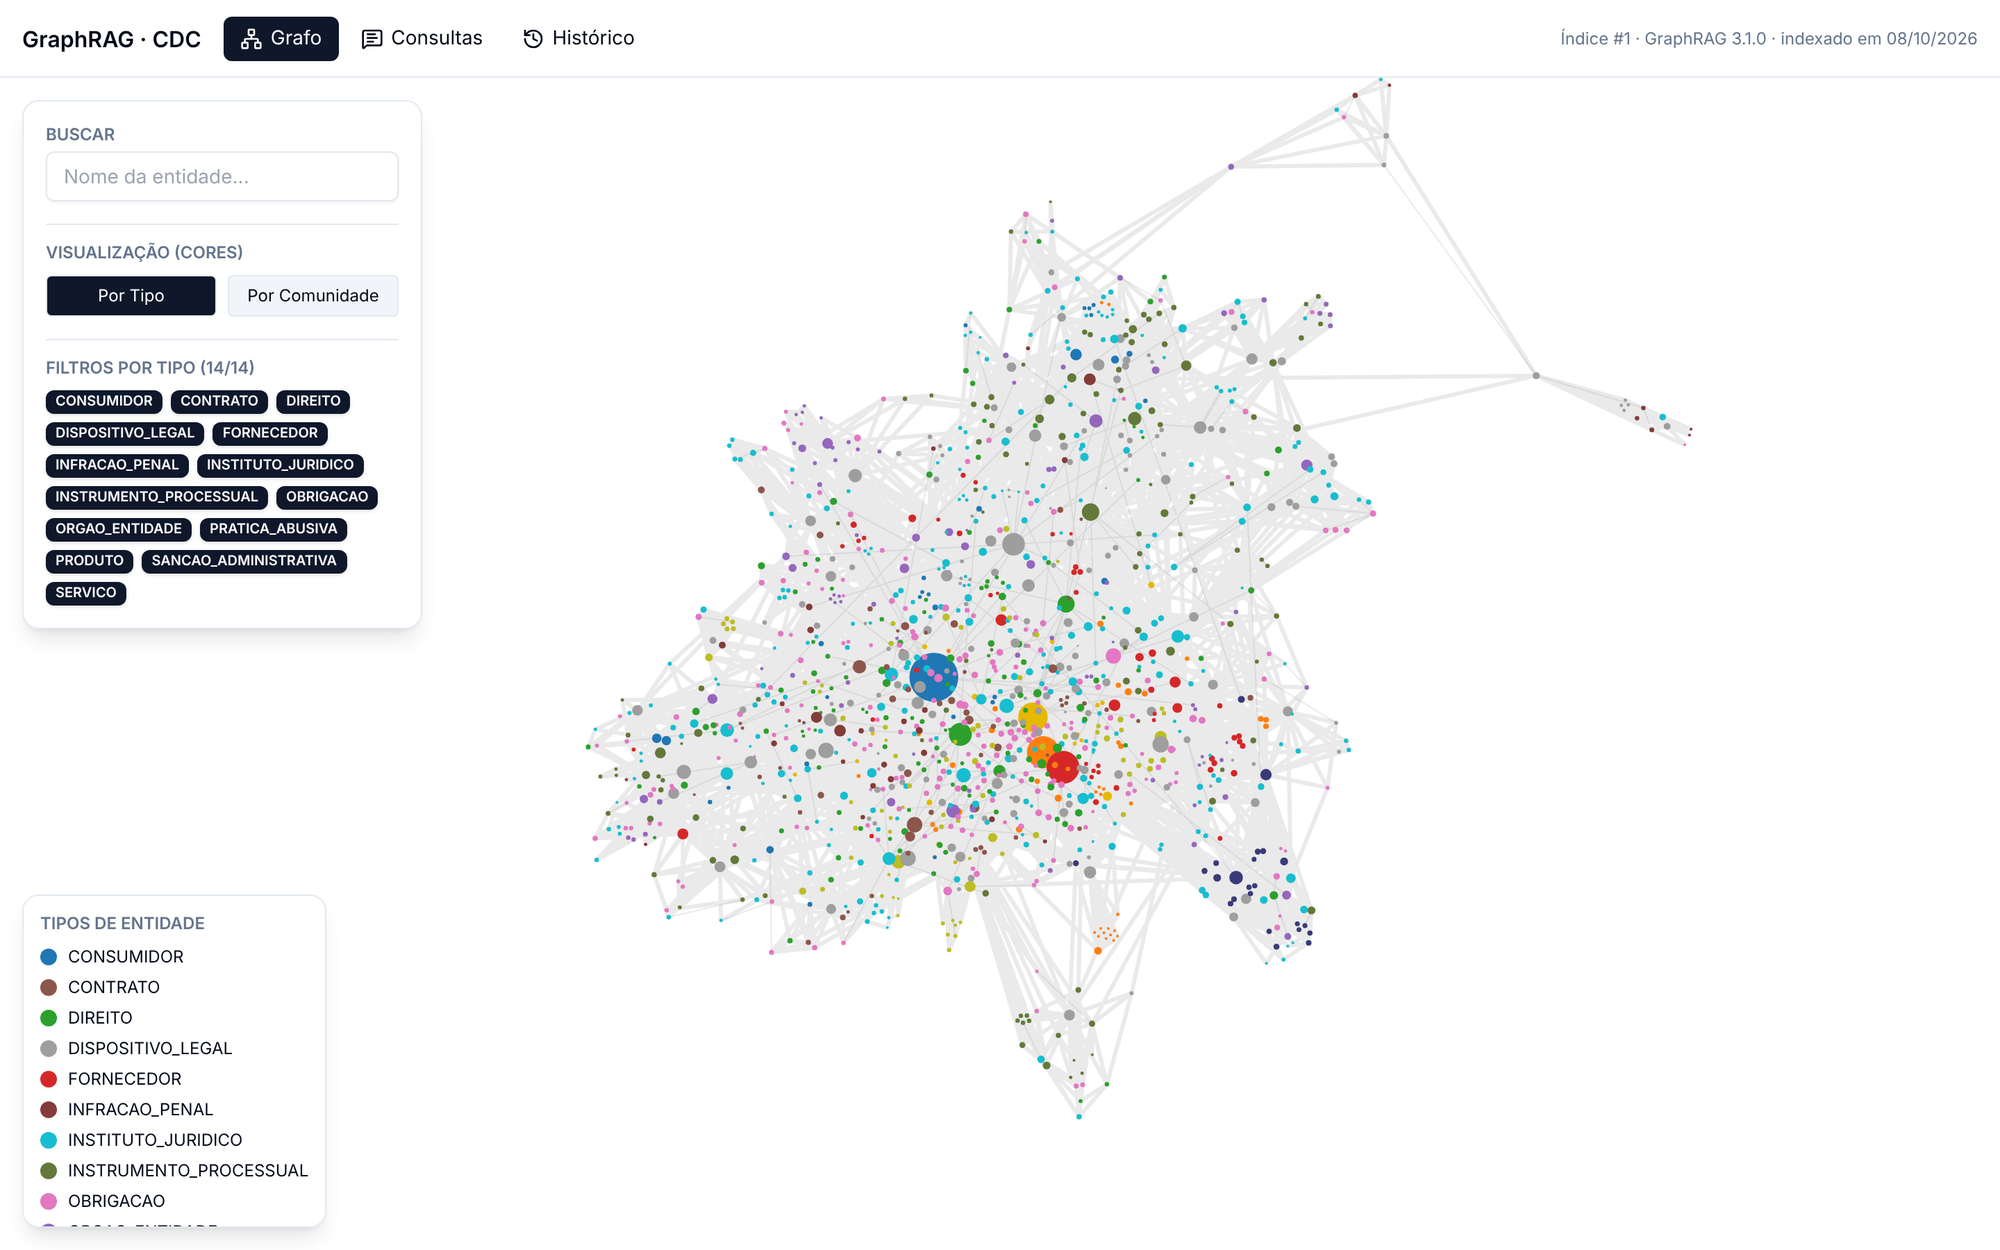
\includegraphics[width=\textwidth]{figuras/fig-app-grafo.png}
\caption{Grafo de conhecimento do CDC na aplicação web, com as entidades coloridas por tipo.}
\label{fig-grafo-completo}
\end{figure}

%%% Início de seção. %%%
\section{Custo da Indexação}
\label{sec-indexacao-custo}

A Tabela~\ref{tab-tokens-indexacao} apresenta o consumo de \textit{tokens} registrado pelo GraphRAG durante a indexação. O modelo principal fez 630 chamadas: 260 de extração (duas por unidade de texto, devido à rodada adicional) e as demais de geração dos 369 relatórios de comunidade. O modelo barato fez 406 chamadas de resumo de descrições.

\begin{table}[htb]
\centering
\caption{Consumo de \textit{tokens} da indexação.}
\label{tab-tokens-indexacao}
\footnotesize
\begin{tabular}{L{4.6cm} r r r}
\toprule
\textbf{Modelo} & \textbf{Chamadas} & \textbf{\textit{Tokens} de entrada} & \textbf{\textit{Tokens} de saída} \\
\midrule
\code{gpt-6.1-sol} & 630 & 4.303.693 & 1.471.243 \\
\code{gpt-6-luna} & 406 & 188.741 & 157.098 \\
\code{text-embedding-3-large} & 220 & 1.032.518 & -- \\
\bottomrule
\end{tabular}
\end{table}

O custo estimado pelos preços de tabela dos modelos ficou entre 16 e 24 dólares, enquanto a estimativa feita antes da indexação, a partir do tamanho do corpus, era de 3 a 6 dólares. A diferença veio principalmente dos \textit{tokens} de saída, os mais caros: a extração foi muito mais detalhada do que o previsto, com mais de 6.800 relações para um corpus de 130 artigos, e cada relação é acompanhada de uma descrição. Além disso, o \textit{prompt} de extração, com cerca de 11,7 mil \textit{tokens}, é enviado em todas as chamadas de extração, e os \textit{tokens} de raciocínio dos modelos utilizados são cobrados mas não aparecem nas contagens. A lição é que o custo do GraphRAG é dominado pela extração do grafo e pelos \textit{tokens} gerados, e que estimativas baseadas apenas no tamanho do corpus o subestimam.

%%% Início de seção. %%%
\section{Publicação e Reprodutibilidade}
\label{sec-indexacao-release}

Para que o índice possa ser reutilizado sem nova indexação, e para que a avaliação seja feita sobre um índice identificado e imutável, o resultado foi publicado como versão (\textit{release}) do repositório no GitHub, com a marcação \code{v0.1.0}, seguindo o versionamento semântico. O pacote contém as pastas de saída, cache e registros da indexação e cópias da configuração, dos \textit{prompts} e do corpus, nos caminhos originais, acompanhado de uma soma de verificação SHA-256, de um manifesto (versão do código, modelos, estatísticas do índice, consumo de \textit{tokens} e \textit{hashes} da configuração e dos \textit{prompts}) e de notas da versão com instruções de restauração. Nenhuma chave de API é incluída, o que foi verificado por busca de padrões de chave no pacote. A marcação \code{v1.0.0} foi reservada para o índice que será usado na avaliação final.

Como o cache das respostas dos modelos faz parte do pacote, quem restaurar a versão pode reexecutar a indexação com a mesma configuração praticamente sem custo, e verificar que o resultado é o mesmo. A versão do GraphRAG foi fixada em 3.1.0 em todos os ambientes, já que tanto o formato dos dados quanto o comportamento das consultas podem mudar entre versões.

% ==============================================================================
% Monografia - Áurea Santos de Oliveira
% Capítulo 5 - Aplicação web
% ==============================================================================
\chapter{Aplicação Web para Exploração e Consulta do Grafo}
\label{sec-aplicacao}

Este capítulo apresenta a aplicação web desenvolvida como parte da prova de conceito. A Seção~\ref{sec-aplicacao-requisitos} descreve seus objetivos e funcionalidades. A Seção~\ref{sec-aplicacao-arquitetura} apresenta a arquitetura e a Seção~\ref{sec-aplicacao-conteineres}, os contêineres. As seções~\ref{sec-aplicacao-backend} a~\ref{sec-aplicacao-frontend} detalham o \textit{backend}, o banco de dados e o \textit{frontend}. Por fim, a Seção~\ref{sec-aplicacao-validacao} descreve a validação funcional da aplicação.

%%% Início de seção. %%%
\section{Objetivos e Funcionalidades}
\label{sec-aplicacao-requisitos}

A primeira versão da aplicação apenas lia os arquivos do índice e exibia o grafo; as consultas eram feitas pela linha de comando, dentro do contêiner do GraphRAG, e mostravam somente a resposta final. Para os objetivos deste trabalho, isso era insuficiente. Comparar as modalidades de busca exige ver \textbf{o que cada uma recupera e envia ao modelo}, e não apenas a resposta, e exige registrar as consultas de forma sistemática, para que possam ser revistas e comparadas. A aplicação foi então reestruturada com os seguintes requisitos funcionais:

\begin{description}
    \item[RF01 -- Visualizar o grafo.] Exibir o grafo de conhecimento completo, de forma interativa, com coloração por tipo de entidade ou por comunidade, filtros por tipo, busca por nome e painel de detalhes de cada entidade, com sua descrição, suas relações e os relatórios das comunidades a que pertence.
    \item[RF02 -- Realizar consultas.] Permitir fazer perguntas em linguagem natural em qualquer das quatro modalidades (local, global, DRIFT e básica), escolhendo o nível de comunidade e o formato da resposta.
    \item[RF03 -- Exibir as etapas da consulta.] Mostrar, à medida que acontecem, as etapas intermediárias de cada consulta: o contexto recuperado (entidades, relações, relatórios e trechos), o \textit{prompt} enviado ao modelo, as respostas parciais (nas modalidades global e DRIFT), a resposta final e as métricas de chamadas, \textit{tokens} e tempo.
    \item[RF04 -- Relacionar a consulta ao grafo.] Destacar no grafo as entidades e relações correspondentes ao contexto de cada consulta.
    \item[RF05 -- Registrar o histórico.] Armazenar cada consulta, com todas as etapas, em banco de dados, e permitir listá-las, filtrá-las, revê-las e excluí-las.
    \item[RF06 -- Preparar a avaliação.] Permitir que consultas sejam disparadas por \textit{scripts} pela mesma interface de programação (API) usada pela interface, identificando sua origem, e prever o armazenamento de perguntas de teste e de notas atribuídas às respostas, para uma avaliação sistemática futura.
\end{description}

E os seguintes requisitos não funcionais:

\begin{description}
    \item[RNF01 -- Fidelidade.] Uma consulta pela aplicação deve ser equivalente à mesma consulta pela CLI do GraphRAG: mesmo índice, mesma configuração, mesmos \textit{prompts} e mesma versão da biblioteca.
    \item[RNF02 -- Rastreabilidade.] Cada consulta deve registrar qual versão do índice e da configuração a respondeu.
    \item[RNF03 -- Reprodutibilidade.] O sistema deve ser executável em qualquer máquina com Docker, com versões fixadas.
    \item[RNF04 -- Uso local.] Como cada consulta gera custos na conta do provedor de modelos, a aplicação destina-se a uso local e não deve ser exposta publicamente com a chave de API configurada.
\end{description}

%%% Início de seção. %%%
\section{Arquitetura}
\label{sec-aplicacao-arquitetura}

A Figura~\ref{fig-arquitetura} apresenta a arquitetura. Há um \textbf{índice único}, a pasta \code{data/}, que contém a configuração, os \textit{prompts}, a chave de API e o resultado da indexação. O contêiner \code{graphrag} escreve nessa pasta ao indexar; o \textit{backend} lê os mesmos arquivos, com a mesma versão da biblioteca e a mesma configuração, o que garante o requisito de fidelidade (RNF01). O \textit{backend} grava o histórico em um banco SQLite em uma pasta separada (\code{storage/}), e o \textit{frontend} se comunica apenas com o \textit{backend}. Ambos os componentes que usam modelos -- o de indexação e o \textit{backend} -- chamam a API do provedor diretamente.

\begin{figure}[htb]
\centering
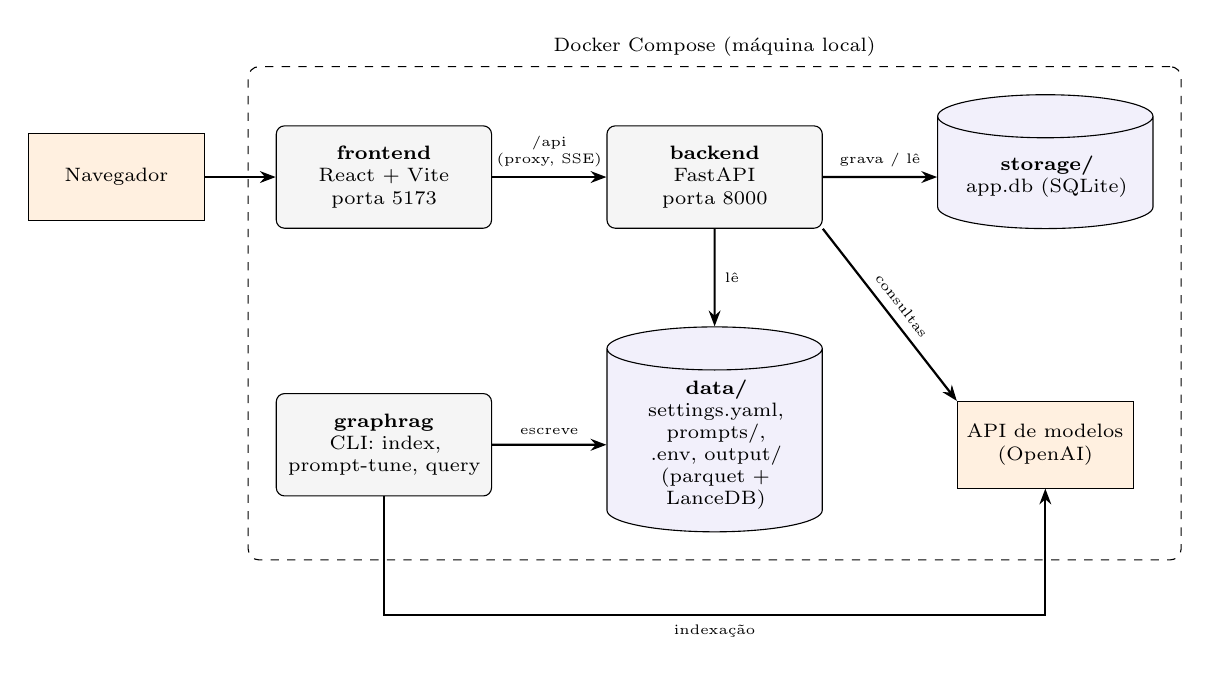
\begin{tikzpicture}[
  svc/.style={draw, rounded corners=3pt, align=center, font=\scriptsize, minimum height=13mm, text width=25mm, fill=gray!8},
  db/.style={draw, cylinder, shape border rotate=90, aspect=0.2, align=center, font=\scriptsize, minimum height=17mm, text width=25mm, fill=blue!6},
  ext/.style={draw, align=center, font=\scriptsize, minimum height=11mm, text width=20mm, fill=orange!12},
  arr/.style={-{Stealth[length=2mm]}, thick},
  lab/.style={font=\tiny, align=center}
]
\node[ext] (nav) at (0,0) {Navegador};
\node[svc] (fe) at (3.4,0) {\textbf{frontend}\\React + Vite\\porta 5173};
\node[svc] (be) at (7.6,0) {\textbf{backend}\\FastAPI\\porta 8000};
\node[db]  (st) at (11.8,0) {\textbf{storage/}\\app.db (SQLite)};
\node[svc] (gr) at (3.4,-3.4) {\textbf{graphrag}\\CLI: index,\\prompt-tune, query};
\node[db]  (data) at (7.6,-3.4) {\textbf{data/}\\settings.yaml, prompts/,\\.env, output/\\(parquet + LanceDB)};
\node[ext] (llm) at (11.8,-3.4) {API de modelos (OpenAI)};
\draw[arr] (nav) -- (fe);
\draw[arr] (fe) -- node[lab, above]{/api\\(proxy, SSE)} (be);
\draw[arr] (be) -- node[lab, above]{grava / lê} (st);
\draw[arr] (be) -- node[lab, right]{lê} (data);
\draw[arr] (gr) -- node[lab, above]{escreve} (data);
\draw[arr] (be.south east) -- node[lab, above, sloped]{consultas} (llm.north west);
\draw[arr] (gr.south) -- ++(0,-1.5) -| node[lab, below, pos=0.25]{indexação} (llm.south);
\begin{scope}[on background layer]
\node[draw, dashed, rounded corners, fit=(fe)(be)(st)(gr)(data), inner sep=3.5mm, label={[font=\scriptsize]above:Docker Compose (máquina local)}] {};
\end{scope}
\end{tikzpicture}
\caption{Arquitetura da aplicação.}
\label{fig-arquitetura}
\end{figure}

A aplicação suporta três fluxos:

\begin{enumerate}
    \item \textbf{Indexação} (rara): executada pela CLI no contêiner \code{graphrag}, gera a pasta \code{data/output}. Após uma nova indexação, o \textit{backend} recarrega o índice por uma rota da API ou ao ser reiniciado.
    \item \textbf{Consulta} (interativa): o navegador envia a pergunta ao \textit{backend}, que monta o motor de busca do GraphRAG, executa a consulta e envia cada etapa ao navegador por SSE, gravando-a ao mesmo tempo no banco.
    \item \textbf{Avaliação} (em lote, prevista para trabalhos futuros): um \textit{script} chama a mesma API para um conjunto de perguntas, modalidades e repetições, identificando as consultas como de avaliação; os resultados são exportados do banco para análise.
\end{enumerate}

%%% Início de seção. %%%
\section{Contêineres e Execução}
\label{sec-aplicacao-conteineres}

O sistema é composto pelos serviços da Tabela~\ref{tab-servicos}, definidos em um único arquivo \code{docker-compose.yml}. As pastas do projeto são montadas nos contêineres como volumes, de modo que o índice, a configuração e o banco persistem fora dos contêineres e são compartilhados entre eles. A versão do GraphRAG é fixada (3.1.0) tanto na imagem de indexação quanto na do \textit{backend}, já que o \textit{backend} utiliza funções internas da biblioteca, que podem mudar entre versões.

\begin{table}[htb]
\centering
\caption{Serviços do Docker Compose.}
\label{tab-servicos}
\footnotesize
\begin{tabular}{L{2.2cm} L{3.4cm} L{3.4cm} L{5.2cm}}
\toprule
\textbf{Serviço} & \textbf{Imagem} & \textbf{Volumes} & \textbf{Função} \\
\midrule
\code{graphrag} & Python 3.11 com \code{graphrag==3.1.0} & \code{data/}, \code{scripts/}, \code{corpus/} & Indexação, ajuste de \textit{prompts}, consultas pela CLI e \textit{scripts} auxiliares. Não é um servidor: é usado sob demanda. \\
\code{backend} & Python 3.11 com FastAPI  & \code{data/}, \code{storage/} & API: grafo, consultas com etapas, histórico e versão do índice (porta 8000). \\
\code{frontend} & Node.js 20 com Vite & código do \textit{frontend} & Interface web (porta 5173); repassa \code{/api} ao \textit{backend}. \\
\code{ollama} & Ollama & modelos locais & Servidor de modelos locais. Só é iniciado com o perfil \code{local}. \\
\bottomrule
\end{tabular}
\end{table}

A chave de API fica no arquivo \code{data/.env}, lido automaticamente pelo GraphRAG e excluído do controle de versão; um modelo do arquivo, sem a chave, acompanha o repositório.
%%% Início de seção. %%%
\section{\textit{Backend}}
\label{sec-aplicacao-backend}

\subsection{Organização}
\label{sec-aplicacao-backend-organizacao}

O \textit{backend} é uma aplicação FastAPI organizada em configuração, modelos de dados, serviços e rotas (Tabela~\ref{tab-backend-modulos}). Ao iniciar, cria as tabelas do banco, se necessário, carrega o índice e registra a versão do índice em uso.

\begin{table}[htb]
\centering
\caption{Módulos do \textit{backend}.}
\label{tab-backend-modulos}
\footnotesize
\begin{tabular}{L{4.4cm} L{9.8cm}}
\toprule
\textbf{Módulo} & \textbf{Responsabilidade} \\
\midrule
\code{config.py} & Caminhos (raiz do GraphRAG e pasta do banco) e parâmetros padrão das consultas, iguais aos da CLI (nível de comunidade 2 e resposta em ``\textit{Multiple Paragraphs}''). \\
\code{db.py}, \code{models.py} & Conexão com o SQLite e definição das tabelas com o SQLAlchemy. \\
\code{services/query\_service.py} & Carrega a configuração, as tabelas do índice e os \textit{prompts}; monta os motores de busca; rastreia e emite as etapas de cada consulta. \\
\code{services/run\_service.py} & Cria o registro da consulta, executa-a em segundo plano, grava as etapas e as repassa ao navegador. \\
\code{services/index\_service.py} & Calcula a impressão digital do índice e registra suas versões. \\
\code{services/graph\_loader.py} & Lê o índice e monta o grafo para visualização. \\
\code{routers/} & Rotas da API: grafo, consultas, histórico e índice. \\
\bottomrule
\end{tabular}
\end{table}

\subsection{Carregamento do índice e montagem dos motores}
\label{sec-aplicacao-backend-carga}

Para garantir a equivalência com a CLI, o \textit{backend} reproduz o que a própria biblioteca faz ao executar \code{graphrag query}: carrega a configuração com a função da biblioteca, a partir da mesma pasta raiz; lê as tabelas do índice com o mesmo leitor de dados; e monta os motores de busca com as mesmas funções de fábrica (\textit{factory}) usadas pela API da biblioteca, com os mesmos parâmetros. Os \textit{prompts} de consulta são lidos a partir da pasta raiz, e não do diretório corrente. Se um arquivo de \textit{prompt} configurado não existir, o \textit{backend} falha com uma mensagem clara, em vez de usar silenciosamente o \textit{prompt} padrão, como faria a biblioteca.

Os motores de busca do GraphRAG oferecem dois métodos: \code{stream\_search}, usado pela CLI, que devolve apenas o texto da resposta à medida que é gerado; e \code{search}, que devolve o resultado completo, incluindo o contexto, o número de chamadas e os \textit{tokens} por etapa. O \textit{backend} usa \code{search}, porque precisa dessas informações para exibi-las e registrá-las. A resposta continua sendo exibida à medida que é gerada, porque \code{search} também notifica cada fragmento de texto gerado.

\subsection{Rastreamento das etapas}
\label{sec-aplicacao-backend-etapas}

O GraphRAG permite registrar objetos de \textit{callback} nos motores de busca, que são notificados em pontos do processamento: quando o contexto é montado, no início e no fim das etapas map e reduce e a cada fragmento de resposta gerado. O \textit{backend} implementa um \textit{callback} que converte cada notificação em um evento, conforme a Tabela~\ref{tab-eventos}.

\begin{table}[htb]
\centering
\caption{Eventos emitidos durante uma consulta.}
\label{tab-eventos}
\footnotesize
\begin{tabular}{L{3.2cm} L{2.6cm} L{8.4cm}}
\toprule
\textbf{Evento} & \textbf{Modalidades} & \textbf{Conteúdo} \\
\midrule
\code{run} & todas & Identificador da consulta, parâmetros e versão do índice. \\
\code{context} & todas & Tabelas recuperadas (entidades, relações, relatórios, trechos) e o texto exato inserido no \textit{prompt}. \\
\code{prompt} & local, básica, global & Mensagem de sistema final e pergunta enviadas ao modelo (na global, o \textit{prompt} da síntese). \\
\code{map\_start}, \code{map\_end} & global & Lotes de relatórios e pontos-chave, com notas, de cada lote. \\
\code{reduce\_start}, \code{reduce\_end} & global, DRIFT & Entrada e saída da síntese; na DRIFT, a árvore de perguntas de acompanhamento. \\
\code{token} & todas & Fragmentos da resposta conforme gerada (não gravado no banco). \\
\code{result} & todas & Resposta final, chamadas ao modelo, \textit{tokens} de entrada e saída por etapa e tempo. \\
\code{error}, \code{done} & todas & Erro ou fim da consulta. \\
\bottomrule
\end{tabular}
\end{table}

Os \textit{callbacks} da biblioteca, porém, não bastam para exibir o contexto antes da resposta: nas buscas local e básica, o GraphRAG só notifica o contexto depois de gerar a resposta (defeito 9 da Tabela~\ref{tab-defeitos}). Para contornar isso sem modificar a biblioteca, o \textit{backend} substitui, na instância do motor criada para cada consulta, o método que monta o contexto por uma versão que chama o método original e, em seguida, emite o contexto e o \textit{prompt} final. O \textit{prompt} é reconstruído com o mesmo modelo de texto e os mesmos argumentos que o GraphRAG usa, de modo que o usuário vê exatamente o que é enviado ao modelo, antes mesmo de a resposta começar.

\subsection{Execução em segundo plano e transmissão}
\label{sec-aplicacao-backend-sse}

Uma consulta começa com uma requisição \code{POST /api/query}. O \textit{backend} cria o registro da consulta no banco, com estado ``em andamento'', e inicia a execução em uma tarefa assíncrona separada da conexão. Cada evento emitido pela tarefa é gravado no banco (exceto os fragmentos de resposta, para não sobrecarregá-lo) e colocado em uma fila, da qual a rota lê e envia os eventos ao navegador no formato SSE. Ao final, o registro recebe a resposta, as métricas e o estado final. Como a gravação acontece na tarefa, e não na conexão, uma consulta iniciada continua e fica registrada mesmo que o navegador seja fechado -- o que é importante para consultas que levam minutos e custam dinheiro. Para uso por \textit{scripts}, a mesma rota aceita um parâmetro que desativa o \textit{streaming} e devolve o registro completo ao final.

Além desses mecanismos, o \textit{backend} contorna, sem modificar a biblioteca, defeitos do GraphRAG que afetariam as consultas, em especial uma falha que faz a busca básica devolver sempre uma resposta vazia quando usada programaticamente. Essas correções estão descritas no documento de observações de implementação do repositório do projeto\footnote{\url{https://github.com/aureaooliveira/graphrag-cdc-explorer/blob/master/docs/observacoes-implementacao.md}}.

\subsection{Versionamento do índice}
\label{sec-aplicacao-backend-versao}

Para atender ao requisito de rastreabilidade (RNF02), o \textit{backend} calcula, ao carregar o índice, uma impressão digital: um \textit{hash} SHA-256 que combina os \textit{hashes} das tabelas principais do índice, do \code{settings.yaml} e de todos os \textit{prompts}. Se qualquer um desses arquivos mudar -- uma reindexação, uma alteração de configuração das buscas ou de um \textit{prompt} --, a impressão digital muda e uma nova versão do índice é registrada no banco, com a data da indexação, os modelos e a versão da biblioteca. Cada consulta guarda a versão que a respondeu. Assim, resultados obtidos com configurações diferentes nunca se misturam nas análises.

\subsection{Rotas da API}
\label{sec-aplicacao-backend-rotas}

A Tabela~\ref{tab-rotas} lista as rotas da API. A documentação interativa é gerada automaticamente pelo FastAPI.

\begin{table}[htb]
\centering
\caption{Rotas da API do \textit{backend}.}
\label{tab-rotas}
\footnotesize
\begin{tabular}{L{1.6cm} L{4.4cm} L{8.2cm}}
\toprule
\textbf{Método} & \textbf{Rota} & \textbf{Descrição} \\
\midrule
GET & \code{/api/graph}, \code{/api/communities}, \code{/api/meta} & Grafo para visualização, comunidades e metadados (tipos, níveis). Cada nó traz as unidades de texto de onde foi extraído. \\
POST & \code{/api/query} & Executa uma consulta e transmite as etapas por SSE (ou devolve o registro completo, sem \textit{streaming}). \\
GET & \code{/api/runs} & Histórico, com filtros por modalidade, origem, estado, rodada de avaliação e texto. \\
GET, DELETE & \code{/api/runs/\{id\}} & Consulta com todas as etapas; exclusão. \\
GET & \code{/api/index} & Versão do índice em uso e estado do serviço de consultas. \\
POST & \code{/api/index/reload} & Recarrega o índice após uma reindexação. \\
GET & \code{/api/health} & Verificação de funcionamento. \\
\bottomrule
\end{tabular}
\end{table}

%%% Início de seção. %%%
\section{Banco de Dados}
\label{sec-aplicacao-banco}

O banco SQLite tem seis tabelas, apresentadas na Figura~\ref{fig-er}. O SQLite foi escolhido por não exigir servidor, ser armazenado em um único arquivo -- fácil de copiar, versionar como resultado e inspecionar -- e ser suficiente para o volume de dados de uma prova de conceito. O banco opera no modo WAL (\textit{write-ahead logging}), que permite leituras simultâneas às gravações feitas pelas consultas em andamento.

\begin{figure}[htbp]
\centering
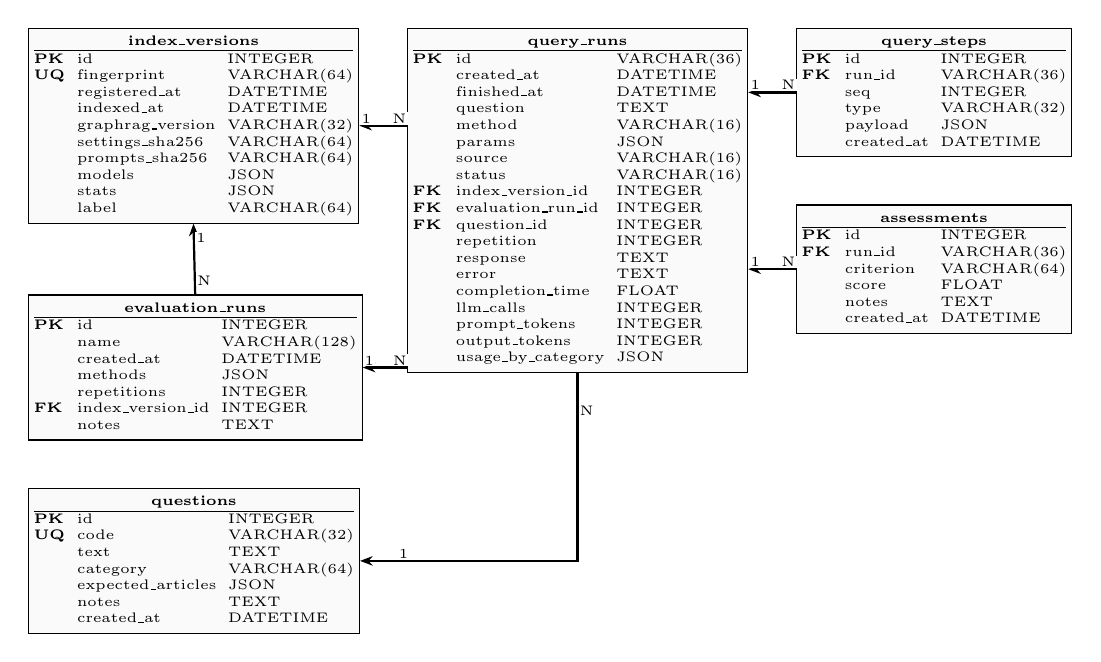
\begin{tikzpicture}[
  tab/.style={draw, fill=gray!4, font=\tiny, inner sep=2pt},
  fk/.style={-{Stealth[length=1.6mm]}, thick},
  card/.style={font=\tiny, fill=white, inner sep=0.5pt}
]
\node[tab, anchor=north west] (iv) at (0,0) {%
\begin{tabular}{@{}p{5.5mm}@{}l@{\hspace{1.5mm}}l@{}}
\multicolumn{3}{c}{\textbf{index\_versions}}\\\hline
\textbf{PK} & id & INTEGER\\
\textbf{UQ} & fingerprint & VARCHAR(64)\\
 & registered\_at & DATETIME\\
 & indexed\_at & DATETIME\\
 & graphrag\_version & VARCHAR(32)\\
 & settings\_sha256 & VARCHAR(64)\\
 & prompts\_sha256 & VARCHAR(64)\\
 & models & JSON\\
 & stats & JSON\\
 & label & VARCHAR(64)
\end{tabular}};
\node[tab, right=6mm of iv.north east, anchor=north west] (qr) {%
\begin{tabular}{@{}p{5.5mm}@{}l@{\hspace{1.5mm}}l@{}}
\multicolumn{3}{c}{\textbf{query\_runs}}\\\hline
\textbf{PK} & id & VARCHAR(36)\\
 & created\_at & DATETIME\\
 & finished\_at & DATETIME\\
 & question & TEXT\\
 & method & VARCHAR(16)\\
 & params & JSON\\
 & source & VARCHAR(16)\\
 & status & VARCHAR(16)\\
\textbf{FK} & index\_version\_id & INTEGER\\
\textbf{FK} & evaluation\_run\_id & INTEGER\\
\textbf{FK} & question\_id & INTEGER\\
 & repetition & INTEGER\\
 & response & TEXT\\
 & error & TEXT\\
 & completion\_time & FLOAT\\
 & llm\_calls & INTEGER\\
 & prompt\_tokens & INTEGER\\
 & output\_tokens & INTEGER\\
 & usage\_by\_category & JSON
\end{tabular}};
\node[tab, below=9mm of iv.south west, anchor=north west] (er) {%
\begin{tabular}{@{}p{5.5mm}@{}l@{\hspace{1.5mm}}l@{}}
\multicolumn{3}{c}{\textbf{evaluation\_runs}}\\\hline
\textbf{PK} & id & INTEGER\\
 & name & VARCHAR(128)\\
 & created\_at & DATETIME\\
 & methods & JSON\\
 & repetitions & INTEGER\\
\textbf{FK} & index\_version\_id & INTEGER\\
 & notes & TEXT
\end{tabular}};
\node[tab, right=6mm of qr.north east, anchor=north west] (qs) {%
\begin{tabular}{@{}p{5.5mm}@{}l@{\hspace{1.5mm}}l@{}}
\multicolumn{3}{c}{\textbf{query\_steps}}\\\hline
\textbf{PK} & id & INTEGER\\
\textbf{FK} & run\_id & VARCHAR(36)\\
 & seq & INTEGER\\
 & type & VARCHAR(32)\\
 & payload & JSON\\
 & created\_at & DATETIME
\end{tabular}};
\node[tab, below=6mm of qs.south west, anchor=north west] (as) {%
\begin{tabular}{@{}p{5.5mm}@{}l@{\hspace{1.5mm}}l@{}}
\multicolumn{3}{c}{\textbf{assessments}}\\\hline
\textbf{PK} & id & INTEGER\\
\textbf{FK} & run\_id & VARCHAR(36)\\
 & criterion & VARCHAR(64)\\
 & score & FLOAT\\
 & notes & TEXT\\
 & created\_at & DATETIME
\end{tabular}};
\node[tab, below=6mm of er.south west, anchor=north west] (qn) {%
\begin{tabular}{@{}p{5.5mm}@{}l@{\hspace{1.5mm}}l@{}}
\multicolumn{3}{c}{\textbf{questions}}\\\hline
\textbf{PK} & id & INTEGER\\
\textbf{UQ} & code & VARCHAR(32)\\
 & text & TEXT\\
 & category & VARCHAR(64)\\
 & expected\_articles & JSON\\
 & notes & TEXT\\
 & created\_at & DATETIME
\end{tabular}};
\draw[fk] (qr.west |- iv.east) -- node[card, pos=0.15, above]{N} node[card, pos=0.85, above]{1} (iv.east);
\draw[fk] (er.north) -- node[card, pos=0.2, right]{N} node[card, pos=0.8, right]{1} (iv.south);
\draw[fk] (qr.west |- er.east) -- node[card, pos=0.15, above]{N} node[card, pos=0.85, above]{1} (er.east);
\draw[fk] (qs.west) -- node[card, pos=0.15, above]{N} node[card, pos=0.85, above]{1} (qr.east |- qs.west);
\draw[fk] (as.west) -- node[card, pos=0.15, above]{N} node[card, pos=0.85, above]{1} (qr.east |- as.west);
\draw[fk] (qr.south) |- node[card, pos=0.1, right]{N} node[card, pos=0.9, above]{1} (qn.east);
\end{tikzpicture}
\caption{Modelo relacional do banco de dados da aplicação. PK: chave primária; FK: chave estrangeira; UQ: valor único. As setas partem da chave estrangeira para a tabela referenciada (cardinalidade N:1).}
\label{fig-er}
\end{figure}

\begin{itemize}
    \item \code{index\_versions}: versões do índice, identificadas pela impressão digital (Seção~\ref{sec-aplicacao-backend-versao});
    \item \code{query\_runs}: uma linha por consulta, com pergunta, modalidade, parâmetros, origem (interface, avaliação ou API), versão do índice, estado, resposta e métricas, inclusive o detalhamento de chamadas e \textit{tokens} por etapa;
    \item \code{query\_steps}: as etapas de cada consulta, na ordem em que ocorreram, com o conteúdo de cada evento em JSON;
    \item \code{questions}, \code{evaluation\_runs} e \code{assessments}: perguntas de teste, rodadas de avaliação (modalidades e repetições) e notas atribuídas às respostas. Essas tabelas já estão criadas, mas serão utilizadas apenas na avaliação comparativa proposta como trabalho futuro.
\end{itemize}

%%% Início de seção. %%%
\section{\textit{Frontend}}
\label{sec-aplicacao-frontend}

O \textit{frontend} é uma aplicação de página única com três abas -- Grafo, Consultas e Histórico -- e um cabeçalho que mostra a versão do índice em uso. O grafo é carregado uma única vez e compartilhado entre as telas.

\subsection{Comunicação com o \textit{backend}}
\label{sec-aplicacao-frontend-proxy}

O servidor do Vite atua como \textit{proxy}: as requisições do navegador para \code{/api} são repassadas ao contêiner do \textit{backend}. Assim, \textit{frontend} e API são vistos pelo navegador como a mesma origem, o que dispensa configuração de compartilhamento entre origens (CORS) e permite o fluxo de eventos. Os eventos SSE são lidos a partir da resposta da requisição de consulta e despachados para o componente que exibe a consulta.

\subsection{Aba Grafo}
\label{sec-aplicacao-frontend-grafo}

A aba Grafo (Figura~\ref{fig-grafo-completo}, no Capítulo~\ref{sec-indexacao}) exibe as 1.373 entidades e 6.885 relações com leiaute por simulação de forças. O tamanho de cada nó é proporcional ao seu grau. O painel lateral permite buscar entidades pelo nome, alternar a coloração entre tipo de entidade e comunidade, com escolha do nível da hierarquia (Figura~\ref{fig-grafo-niveis}), e filtrar os tipos exibidos. Ao passar o cursor sobre uma relação, são exibidos sua descrição e seu peso.

Ao clicar em uma entidade, a visualização é centralizada nela e um painel lateral mostra o nome, o tipo, o grau, a descrição consolidada e os resumos dos relatórios das comunidades a que a entidade pertence em cada nível da hierarquia. A Figura~\ref{fig-app-entidade} mostra o painel da entidade ``DIREITO DE ARREPENDIMENTO'', com os tipos exibidos restritos a cinco por meio dos filtros. A descrição reúne o que foi extraído de dois artigos distintos -- o art. 49 e o art. 54-F, sobre contratos conexos --, e os relatórios mostram que, nos níveis 0 e 1, a entidade pertence a comunidades organizadas em torno do crédito ao consumidor e do superendividamento, e não da proteção contratual geral, o que só se percebe pelo grafo.

\begin{figure}[htb]
\centering
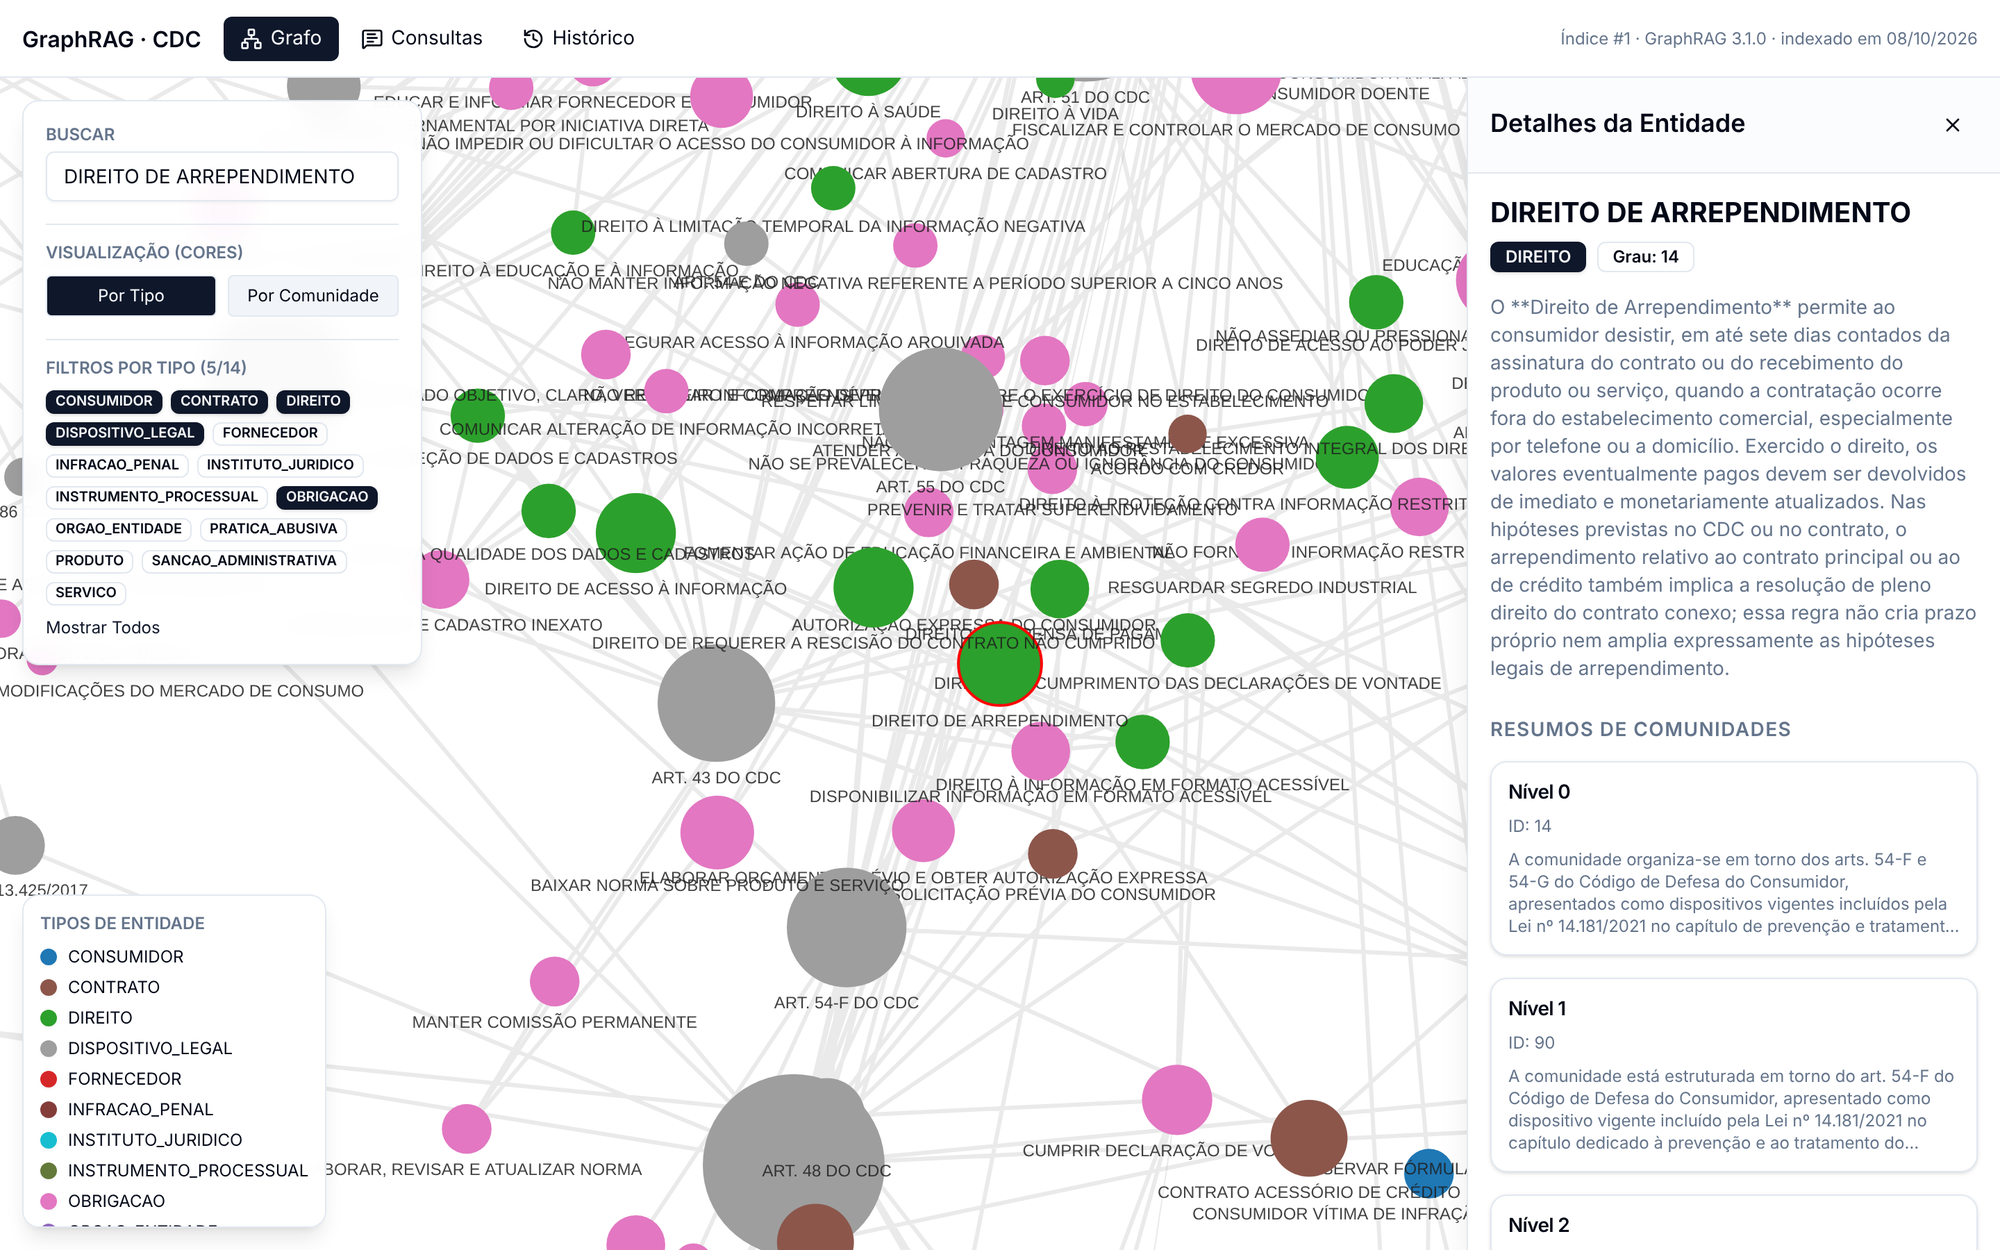
\includegraphics[width=.85\textwidth]{figuras/fig-app-entidade.png}
\caption{Painel de detalhes da entidade ``DIREITO DE ARREPENDIMENTO'': tipo, grau, descrição consolidada e resumos das comunidades a que pertence em cada nível.}
\label{fig-app-entidade}
\end{figure}

A Figura~\ref{fig-grafo-niveis} mostra o grafo colorido por comunidade nos níveis 0, 1 e 2 da hierarquia. No nível 0, as 17 comunidades formam regiões contíguas e bem delimitadas; nos níveis seguintes, as mesmas regiões se subdividem em comunidades menores. As entidades em cinza são as que não pertencem a nenhuma comunidade do nível escolhido: os níveis 0 e 1 cobrem 1.371 das 1.373 entidades (as duas restantes estão fora do maior componente conexo, ao qual a detecção de comunidades se restringe), enquanto o nível 2 cobre 85\% e o nível 3, apenas 24\%, porque só as comunidades maiores que o tamanho máximo são subdivididas. A primeira versão da coloração atribuía cores quase iguais a comunidades de identificadores próximos, problema corrigido com uma paleta fixa para os tipos e cores distribuídas pelo ângulo áureo para as comunidades.

\begin{figure}[htb]
\centering
\begin{minipage}[t]{0.32\textwidth}\centering
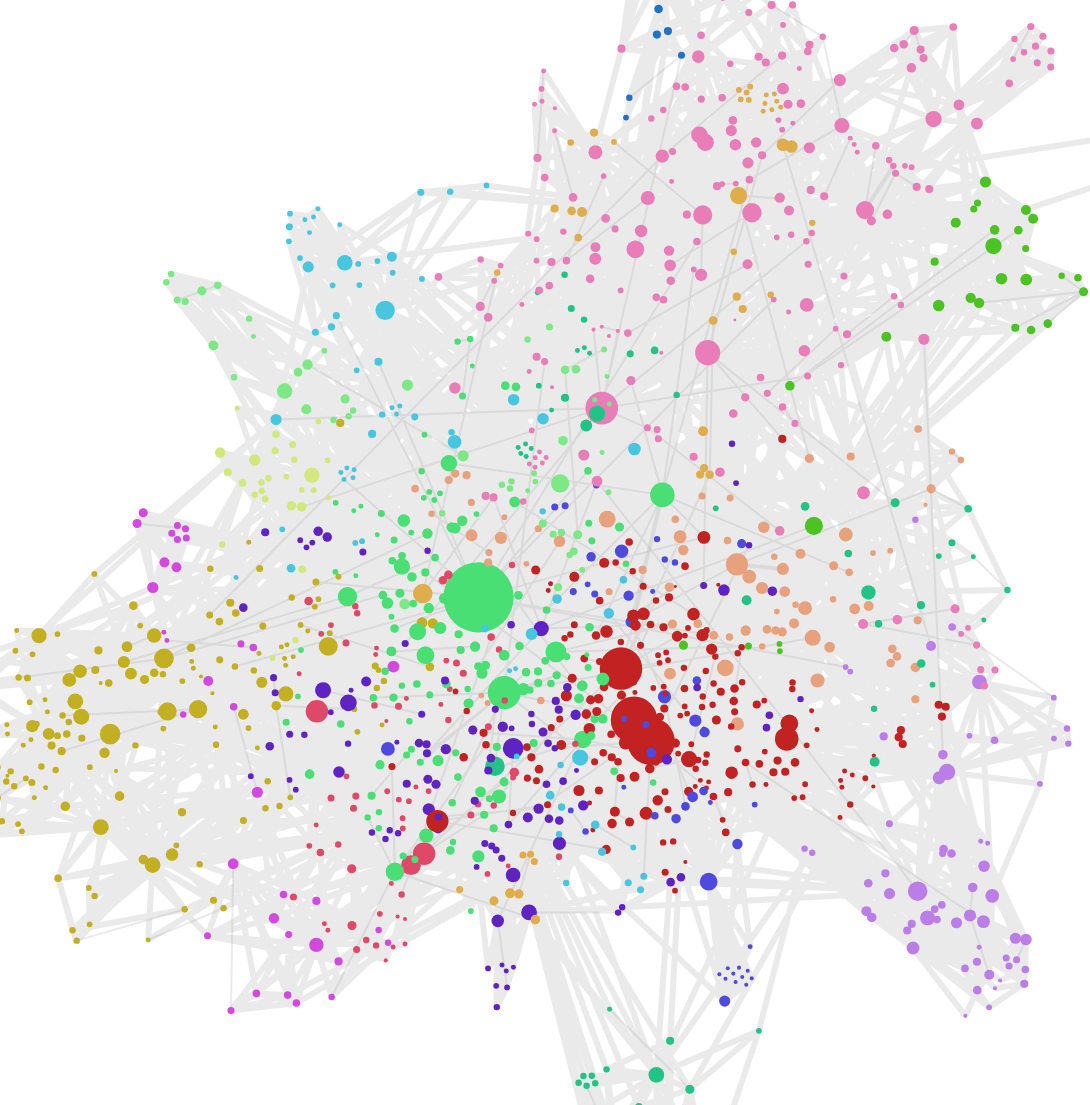
\includegraphics[width=\textwidth]{figuras/fig-grafo-nivel0.png}\\[-1mm]{\footnotesize (a) Nível 0: 17 comunidades}
\end{minipage}\hfill
\begin{minipage}[t]{0.32\textwidth}\centering
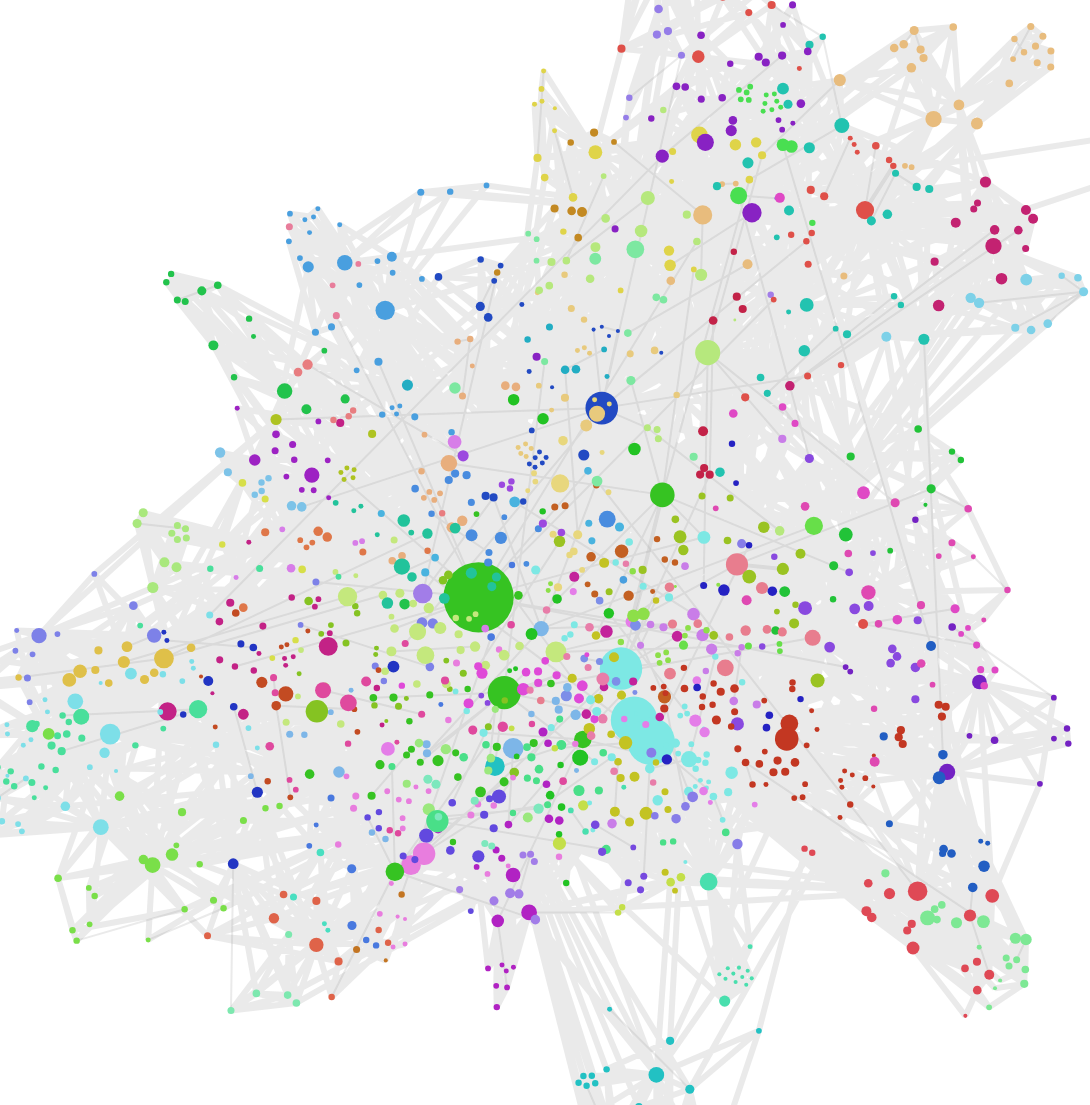
\includegraphics[width=\textwidth]{figuras/fig-grafo-nivel1.png}\\[-1mm]{\footnotesize (b) Nível 1: 89 comunidades}
\end{minipage}\hfill
\begin{minipage}[t]{0.32\textwidth}\centering
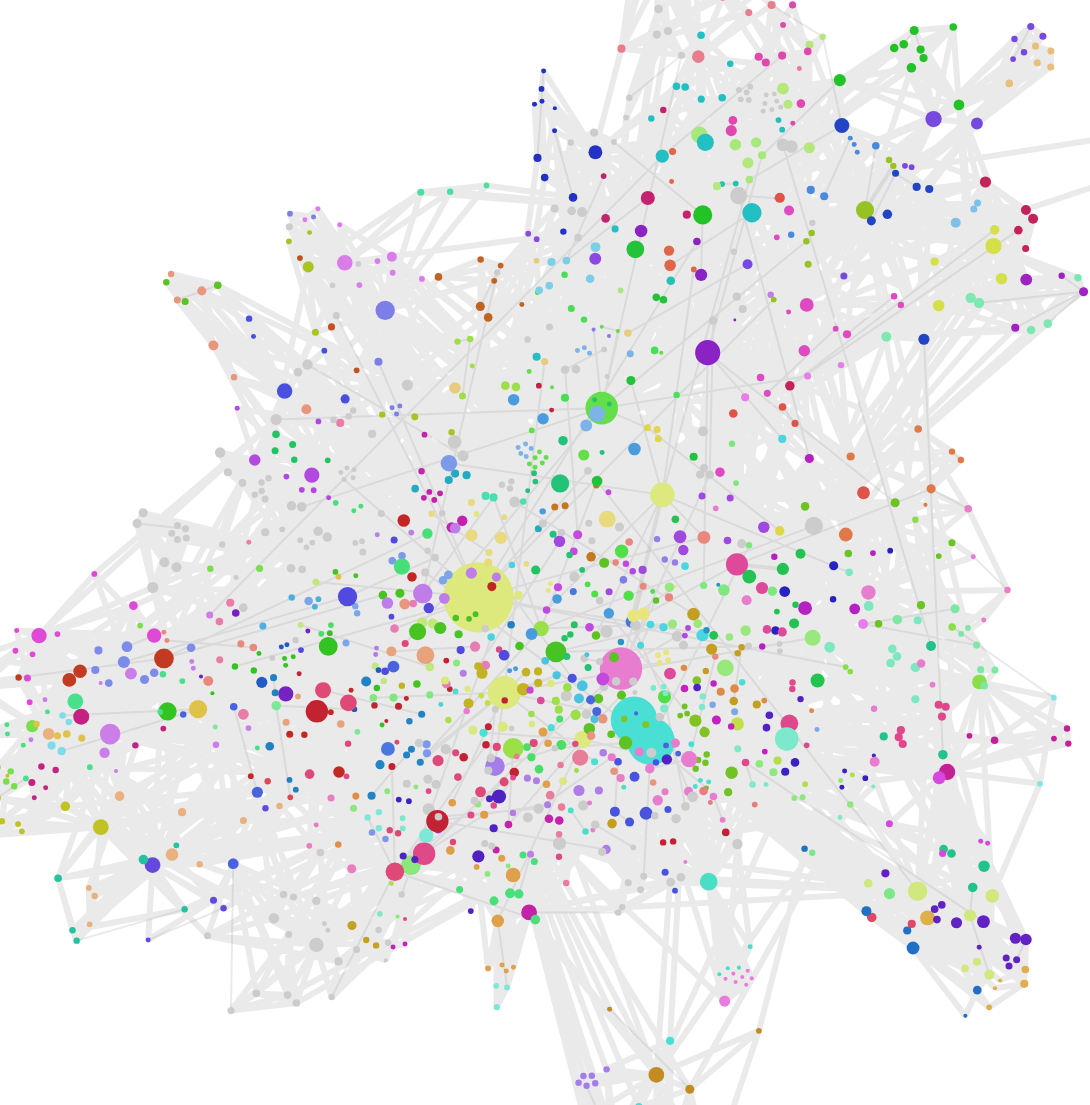
\includegraphics[width=\textwidth]{figuras/fig-grafo-nivel2.png}\\[-1mm]{\footnotesize (c) Nível 2: 185 comunidades}
\end{minipage}
\caption{Região central do grafo do CDC colorida por comunidade em três níveis da hierarquia (mesmo enquadramento nas três imagens). Em cinza, as entidades que não pertencem a nenhuma comunidade do nível.}
\label{fig-grafo-niveis}
\end{figure}

\subsection{Aba Consultas}
\label{sec-aplicacao-frontend-consultas}

A aba Consultas (Figura~\ref{fig-app-consultas}) tem um formulário com a pergunta, a modalidade (com uma descrição de cada uma), o nível de comunidade, com um aviso de custo quando a busca global é escolhida, e o formato da resposta, além de perguntas de exemplo. Ao enviar, a consulta é exibida como uma linha do tempo de etapas recolhíveis, que se completam à medida que os eventos chegam (Figura~\ref{fig-app-local}). As etapas variam conforme a modalidade:

\begin{itemize}
    \item \textbf{Recuperação de contexto} (local, básica e DRIFT; na global, \textbf{relatórios considerados}): o contexto em abas -- entidades, relações, relatórios, trechos e o texto exato enviado ao modelo (Figura~\ref{fig-app-contexto});
    \item \textbf{Map} (global): os pontos-chave de cada lote, ordenados pela nota e com o lote de origem;
    \item \textbf{Subgrafo usado como contexto}: o destaque no grafo, descrito a seguir;
    \item \textbf{Raciocínio DRIFT} (DRIFT): a árvore de perguntas de acompanhamento, com a resposta parcial de cada uma;
    \item \textbf{\textit{Prompt} enviado ao modelo} (local, básica e global): a mensagem de sistema completa e a pergunta, com botão para copiar;
    \item \textbf{Resposta}: exibida à medida que é gerada, com formatação;
    \item \textbf{Métricas}: chamadas ao modelo, \textit{tokens} de entrada e de saída e tempo, no total e por etapa.
\end{itemize}

\begin{figure}[htb]
\centering
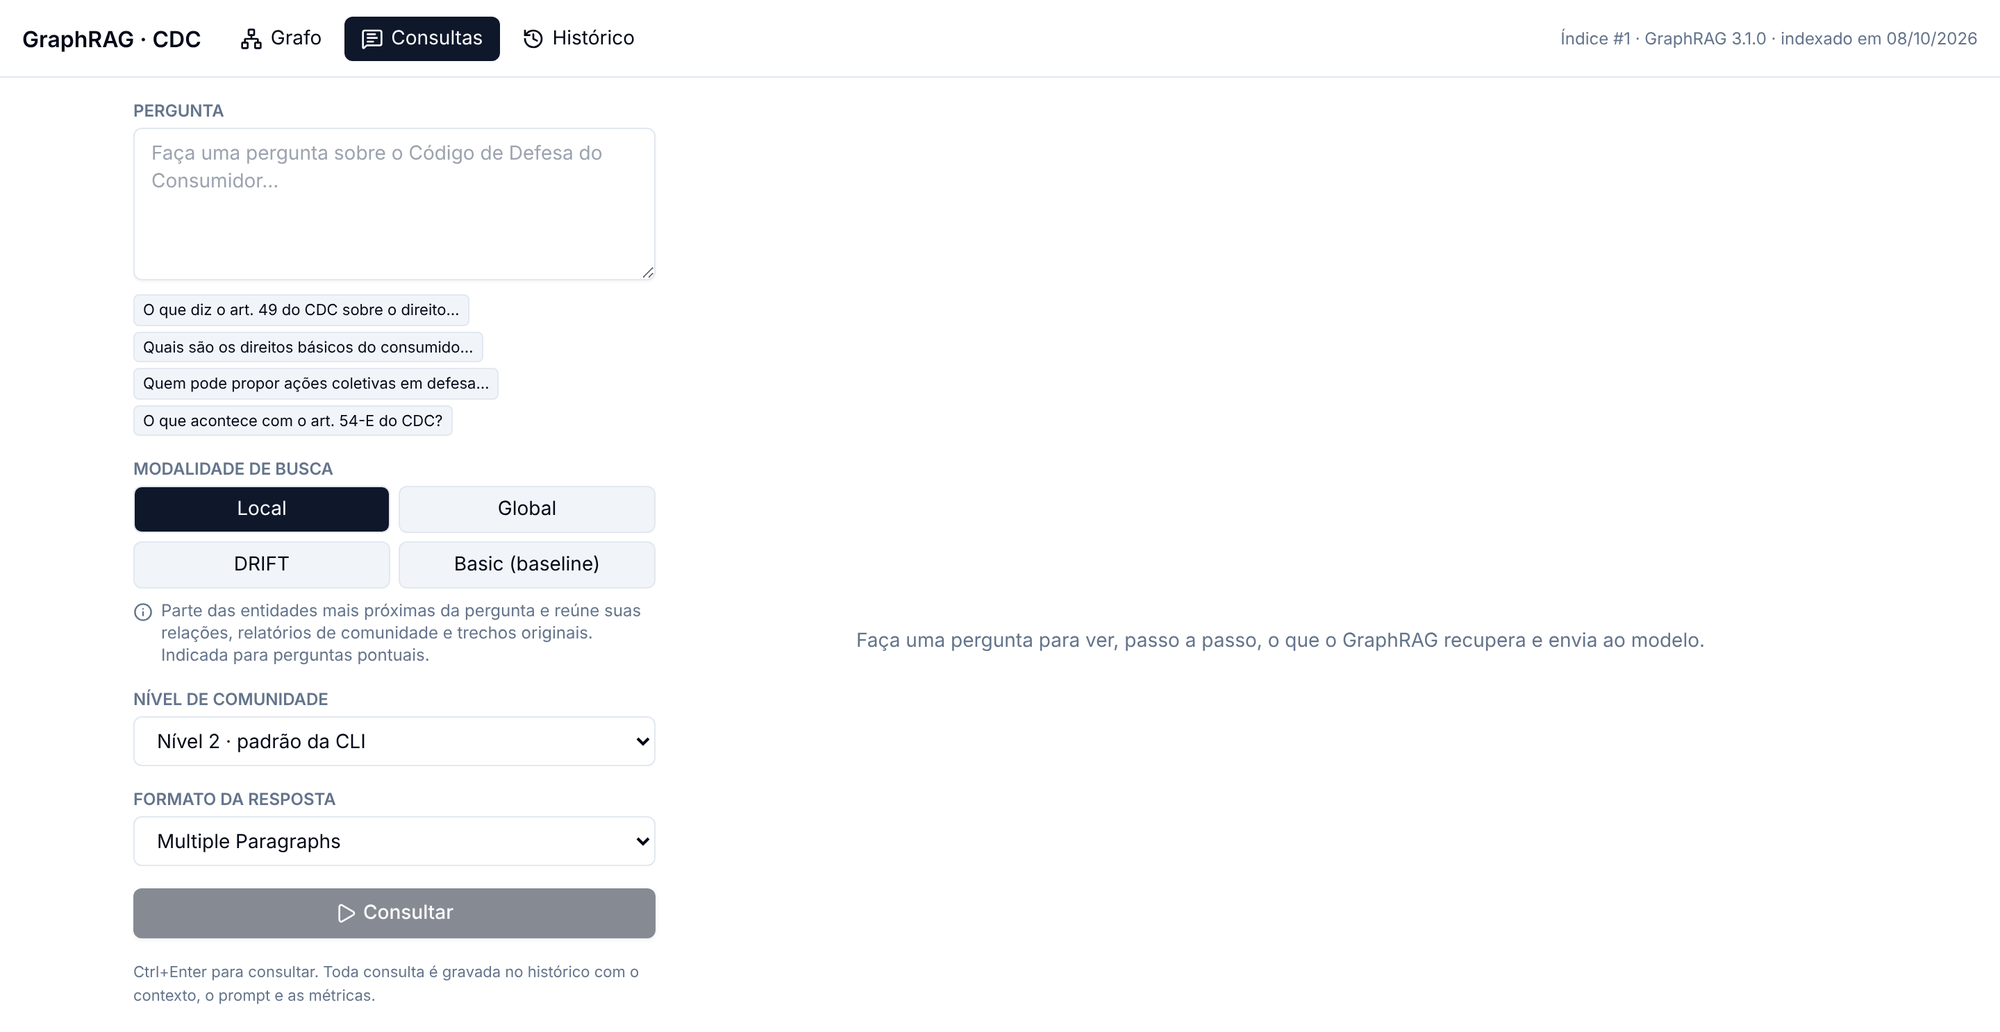
\includegraphics[width=.75\textwidth]{figuras/fig-app-consultas.png}
\caption{Aba Consultas: formulário com modalidade, nível de comunidade, formato da resposta e perguntas de exemplo.}
\label{fig-app-consultas}
\end{figure}

\begin{figure}[htbp]
\centering
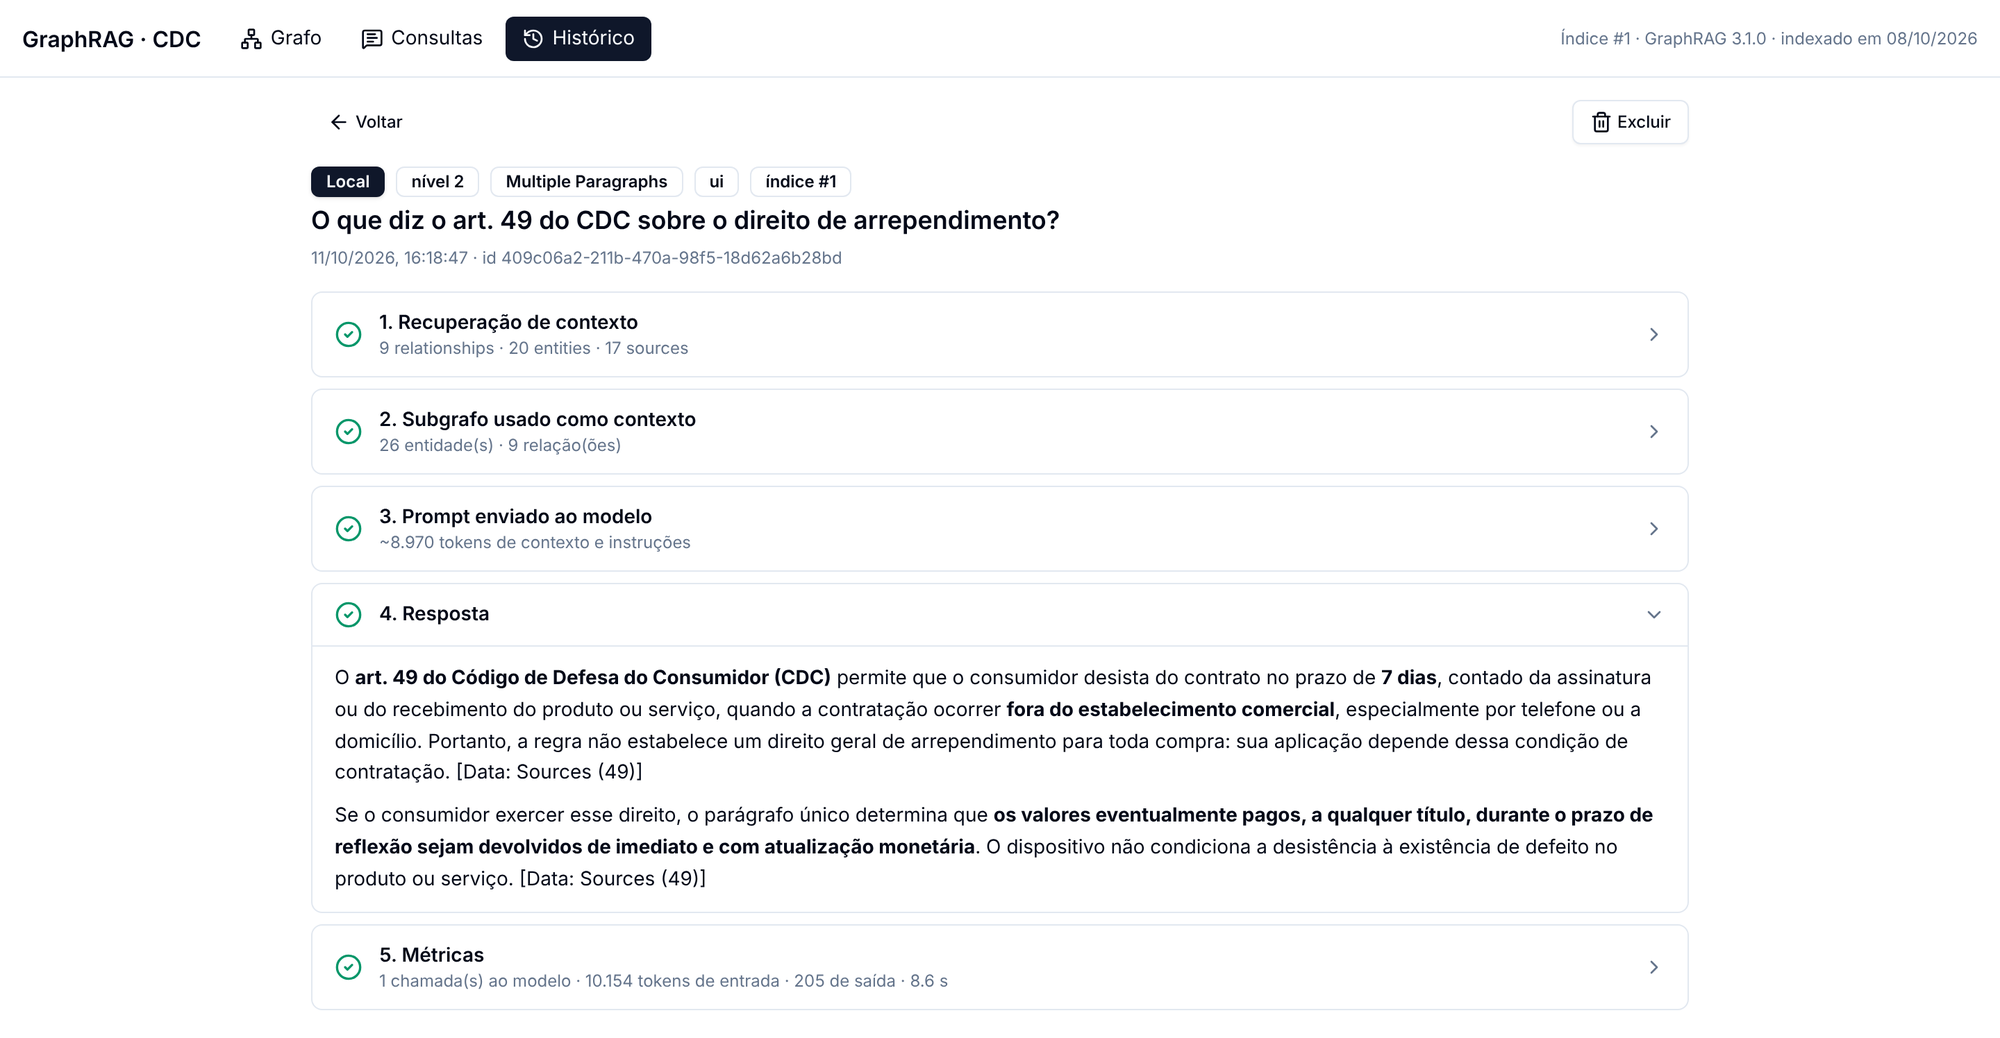
\includegraphics[width=.7\textwidth]{figuras/fig-app-local-resumo.png}
\caption{Linha do tempo de uma consulta real na busca local: etapas recolhíveis, resposta com citações e métricas.}
\label{fig-app-local}
\end{figure}

\begin{figure}[htbp]
\centering
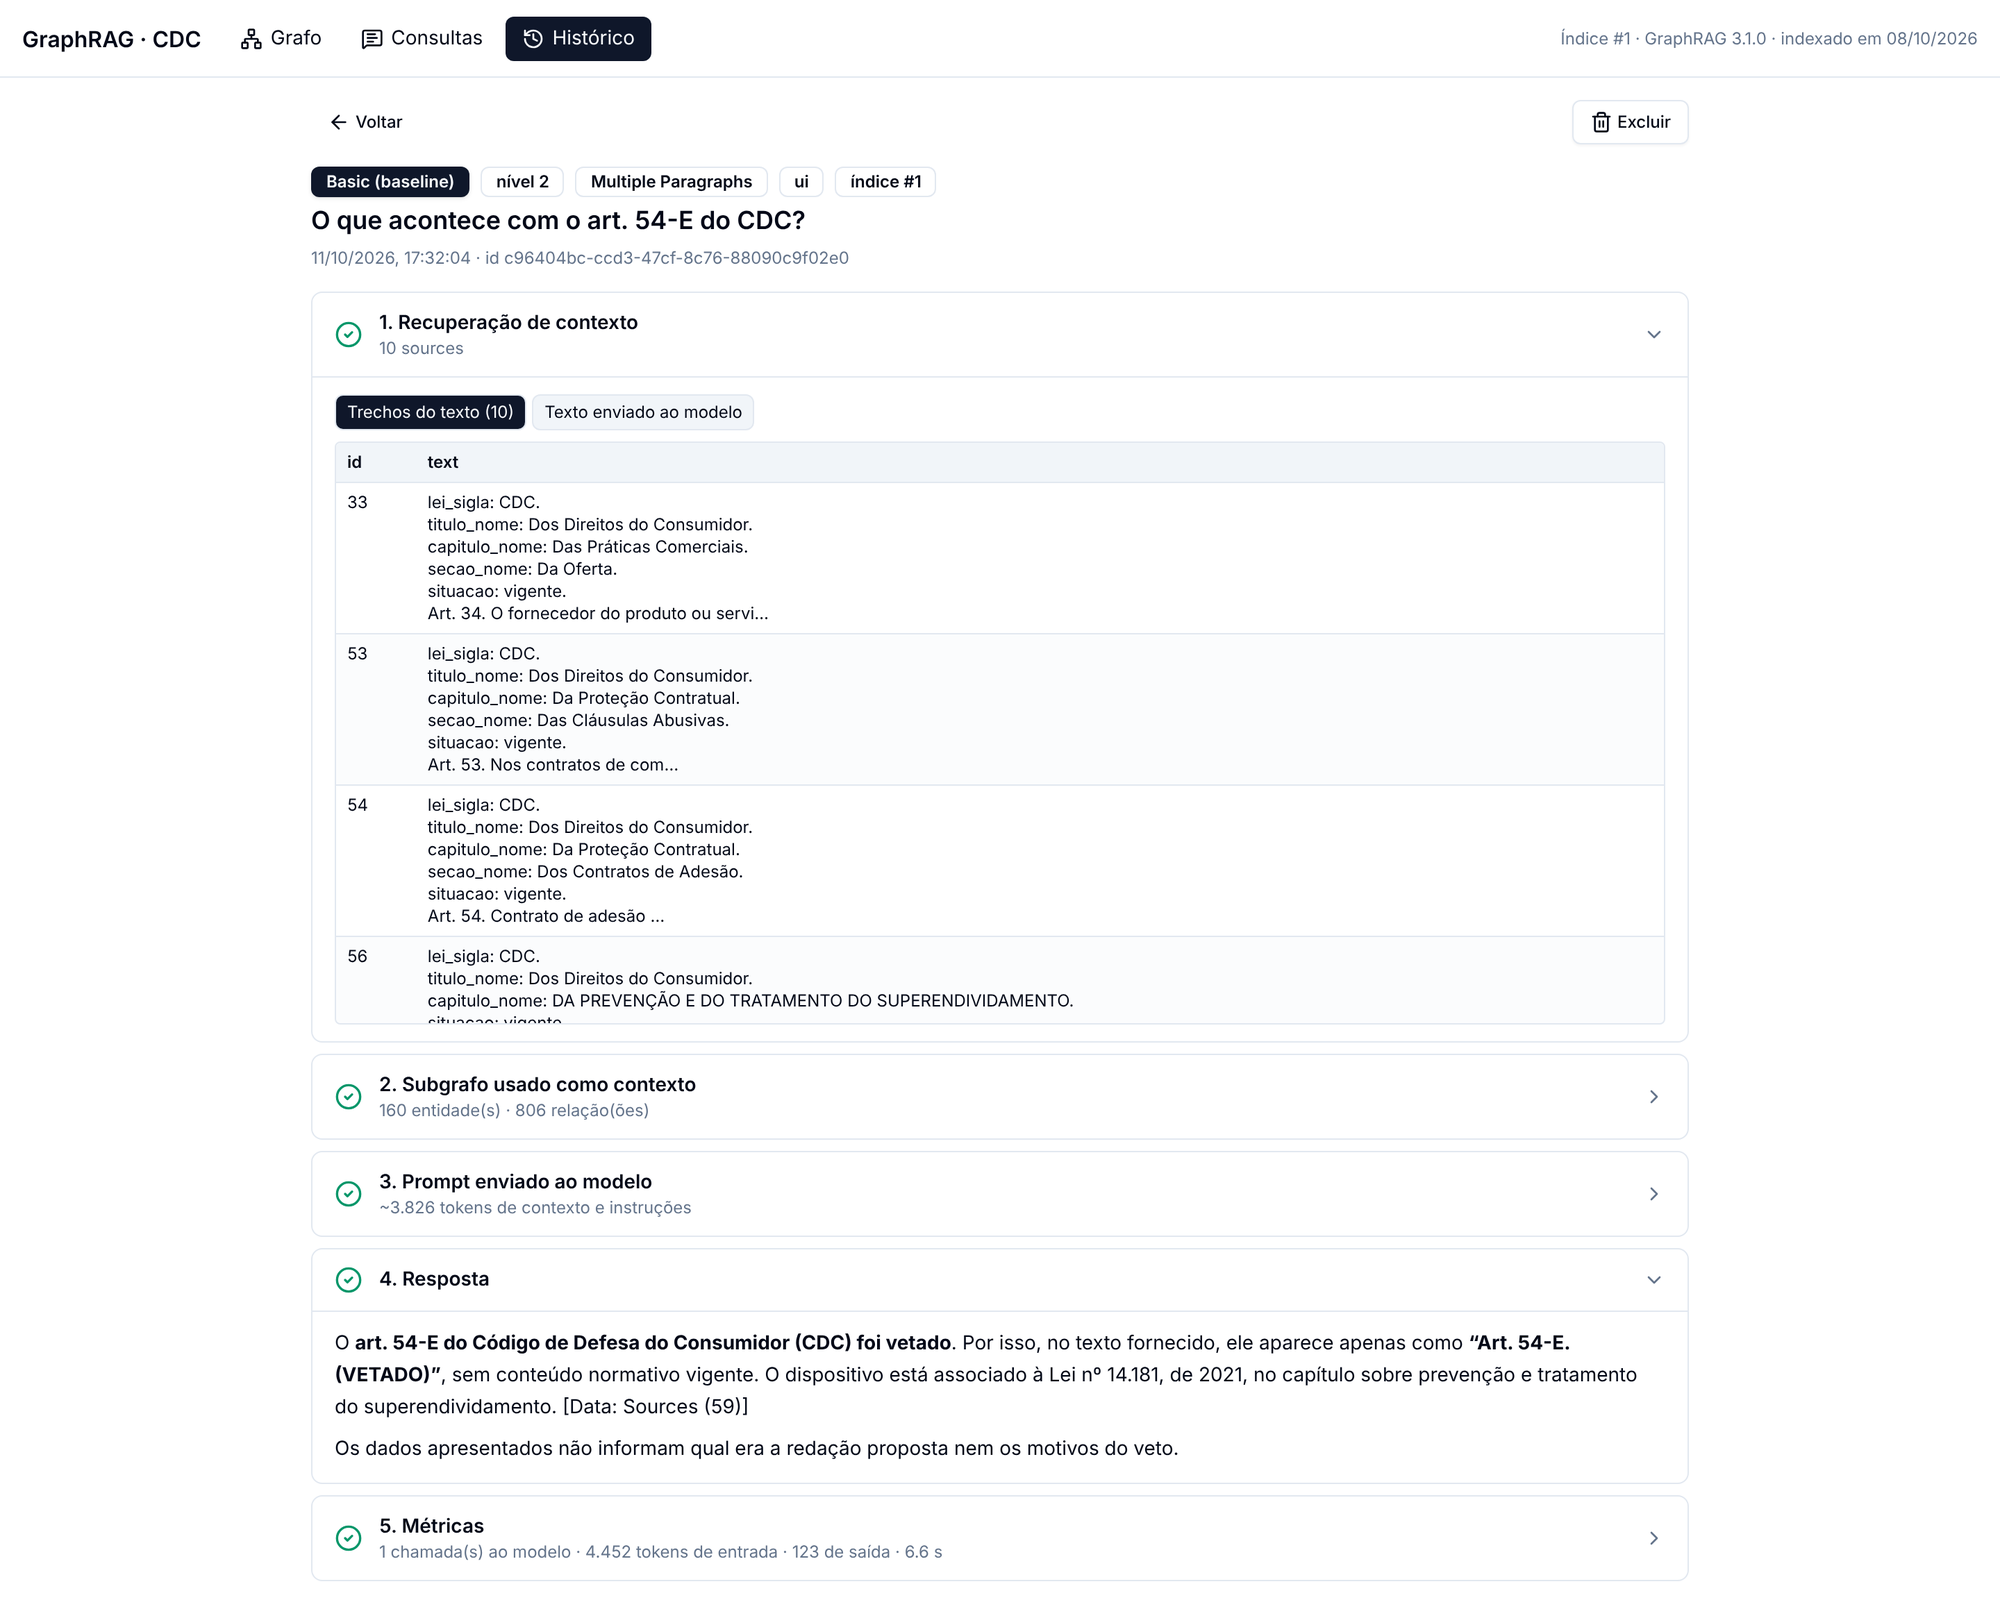
\includegraphics[width=.7\textwidth]{figuras/fig-app-basic-contexto.png}
\caption{Contexto recuperado por uma consulta real na busca básica: os trechos (artigos) recuperados por similaridade, na ordem em que são enviados ao modelo.}
\label{fig-app-contexto}
\end{figure}

\subsection{Aba Histórico}
\label{sec-aplicacao-frontend-historico}

A aba Histórico (Figura~\ref{fig-app-historico}) lista as consultas registradas, com data, modalidade, pergunta, estado, número de chamadas, \textit{tokens} e tempo, e permite filtrar por modalidade, origem e texto. Ao abrir uma consulta, a mesma linha do tempo da aba Consultas é reconstruída a partir das etapas gravadas no banco.

\begin{figure}[htb]
\centering
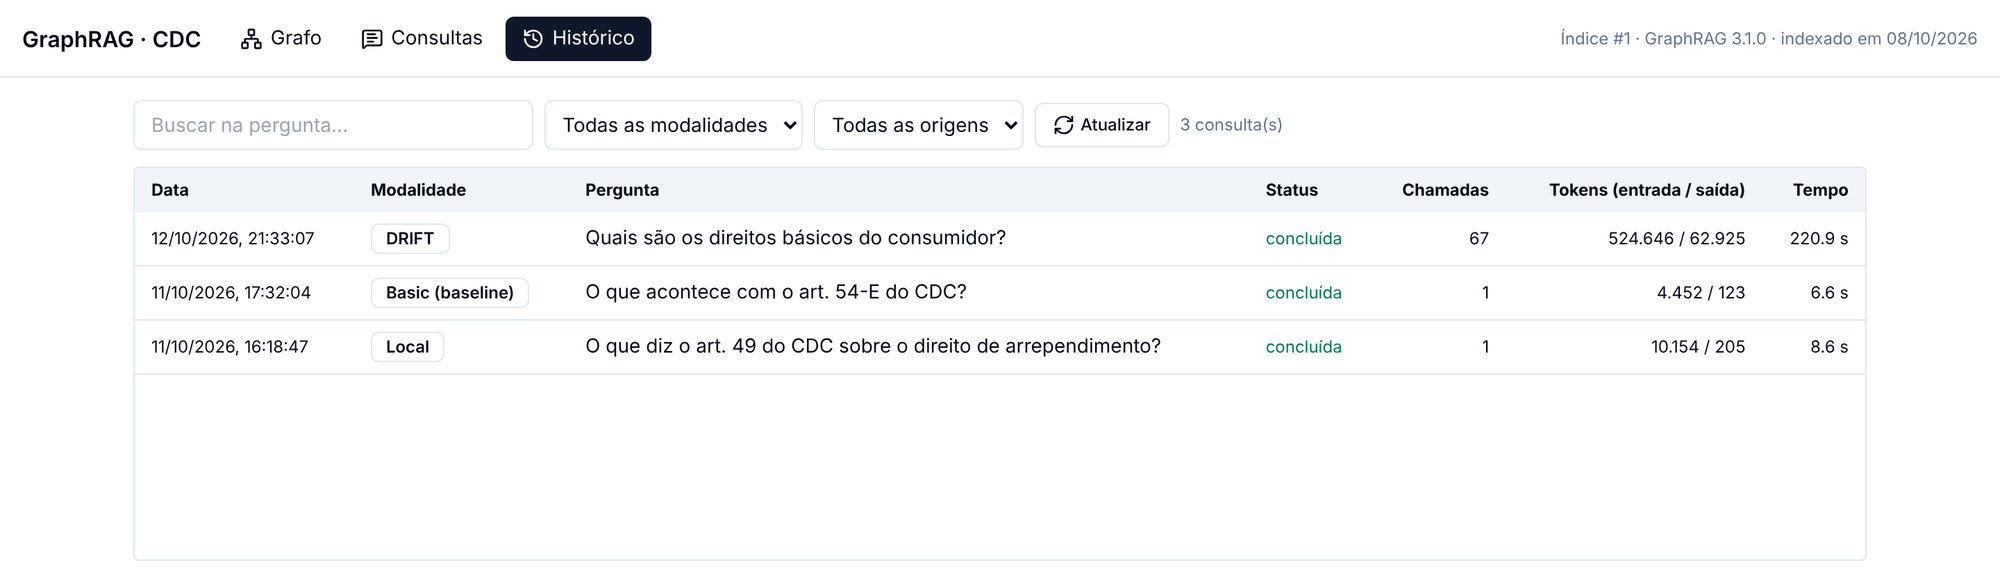
\includegraphics[width=.8\textwidth]{figuras/fig-app-historico.png}
\caption{Aba Histórico com consultas reais nas buscas DRIFT, básica e local.}
\label{fig-app-historico}
\end{figure}

\subsection{Destaque do contexto no grafo}
\label{sec-aplicacao-frontend-destaque}

Para apoiar a análise qualitativa -- entender por que uma resposta saiu mais ou menos completa --, cada consulta mostra qual parte do grafo corresponde ao seu contexto, em duas formas: um subgrafo interativo na própria linha do tempo e, pelo botão ``Ver no grafo completo'', o destaque dessas entidades e relações no grafo inteiro, com as demais esmaecidas, as relações destacadas em vermelho e o enquadramento automático nos nós destacados (Figura~\ref{fig-app-destaque}).

\begin{figure}[htb]
\centering
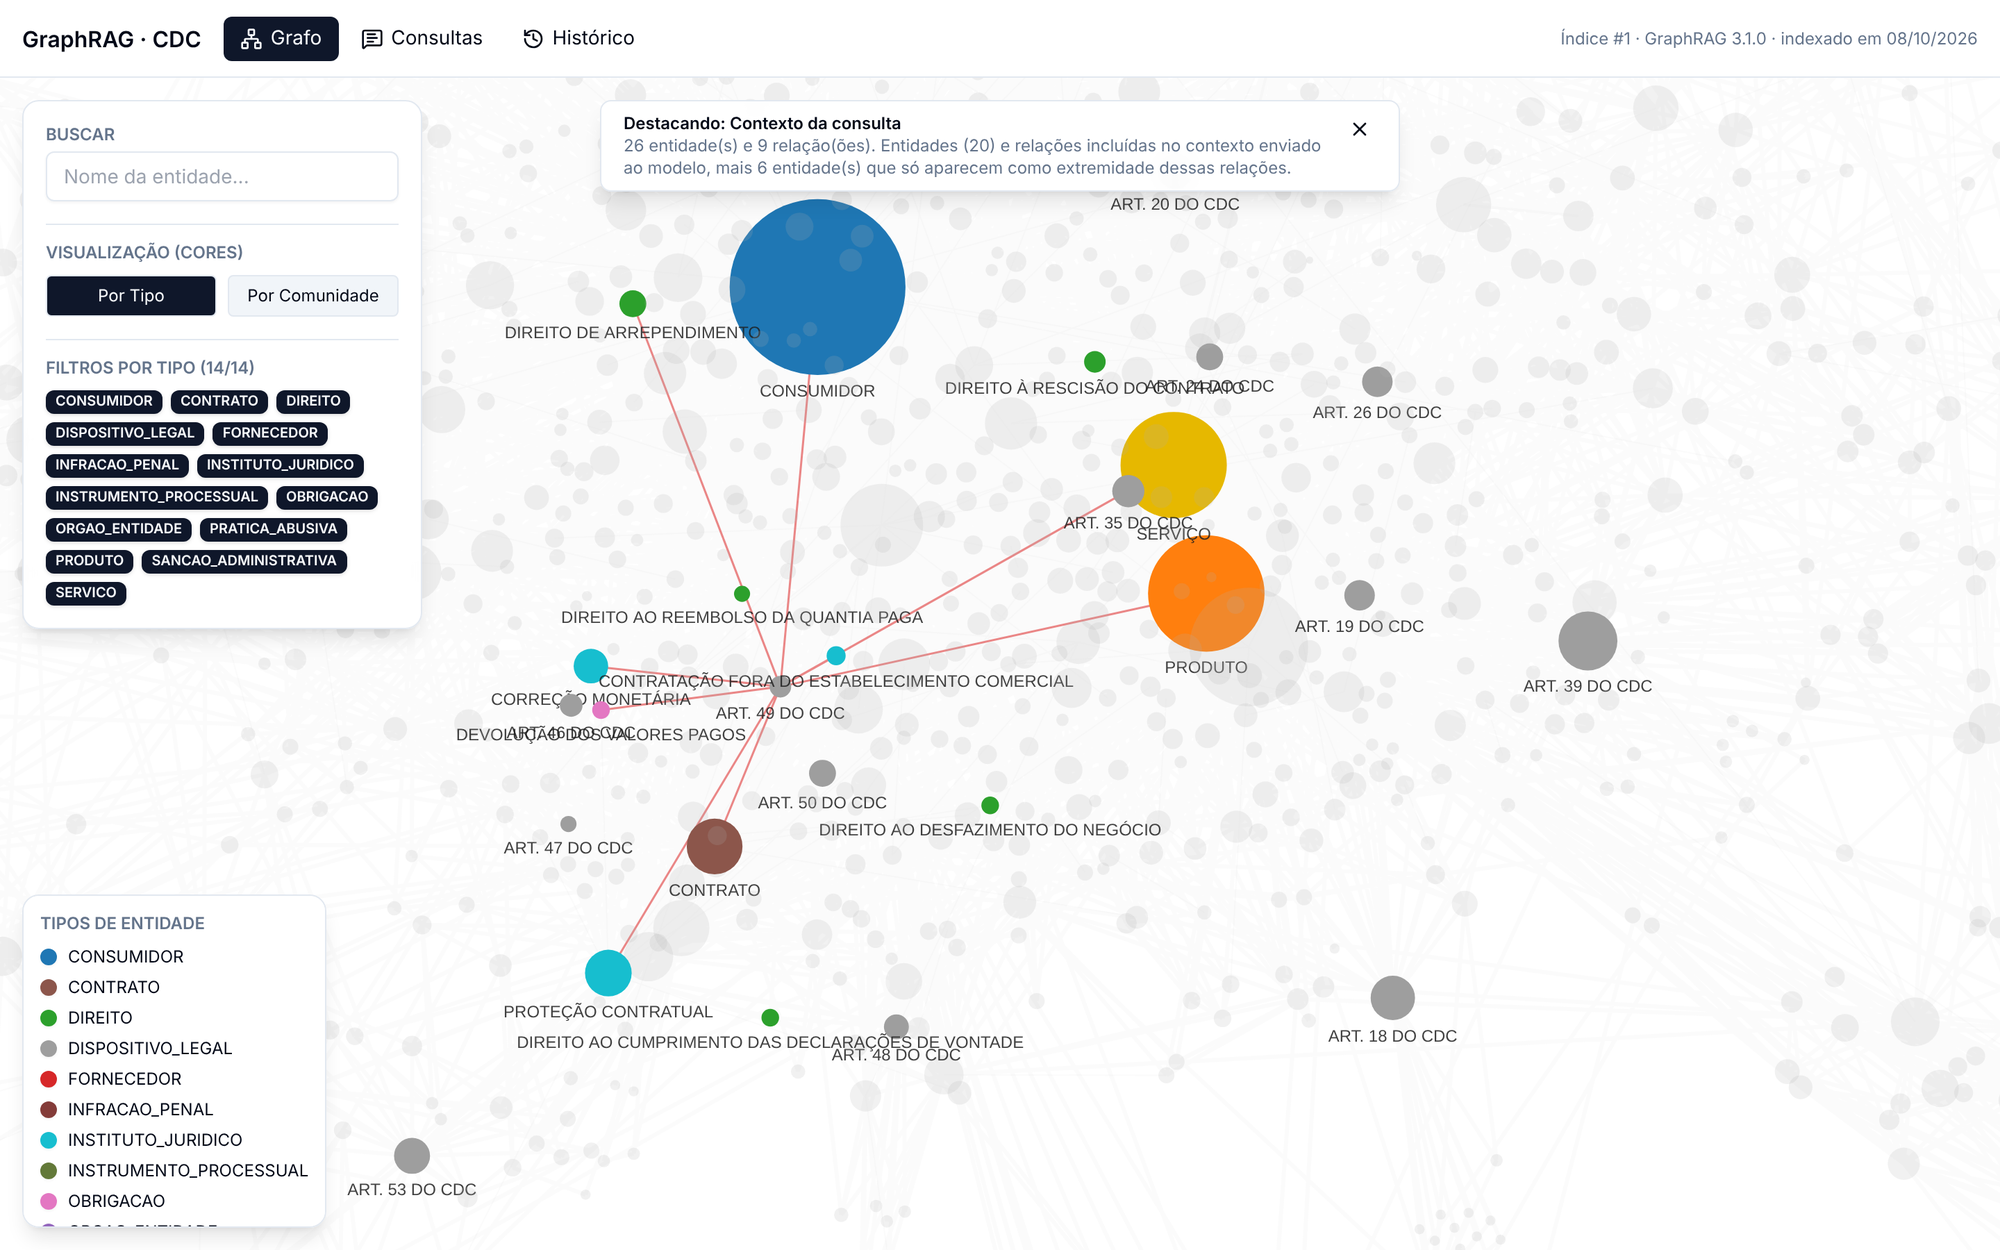
\includegraphics[width=.85\textwidth]{figuras/fig-app-destaque.png}
\caption{Destaque, no grafo completo, das entidades e relações usadas como contexto em uma consulta real na busca local sobre o art. 49 do CDC.}
\label{fig-app-destaque}
\end{figure}

O cálculo depende da modalidade, porque cada uma recupera um tipo diferente de informação:

\begin{itemize}
    \item \textbf{Local e DRIFT}: as entidades da tabela de entidades do contexto, localizadas no grafo pelo nome, e as relações da tabela de relações, incluindo as entidades que só aparecem como extremidade dessas relações. Na DRIFT, usa-se o contexto da primeira busca local, pois a biblioteca não expõe o contexto de cada pergunta de acompanhamento.
    \item \textbf{Básica}: a busca básica não usa o grafo; o destaque mostra as entidades \textbf{extraídas dos trechos recuperados}, isto é, o que o grafo sabe sobre os mesmos trechos que o modelo recebeu como texto. Para isso, o \textit{backend} passou a informar, para cada nó do grafo, os identificadores curtos das unidades de texto de onde a entidade foi extraída -- os mesmos que aparecem no contexto e nas citações (por exemplo, a entidade ``ART. 54-E DO CDC'' aponta para a unidade 59, a mesma citada pela busca básica na pergunta sobre esse artigo).
    \item \textbf{Global}: as entidades das comunidades cujos relatórios foram citados nos pontos-chave relevantes da etapa map e na resposta final.
\end{itemize}

O uso desse destaque na análise de consultas reais é apresentado no Capítulo~\ref{sec-analise}.

%%% Início de seção. %%%
\section{Validação Funcional}
\label{sec-aplicacao-validacao}


Para validar as funcionalidades implementadas, foram feitas consultas reais, com custo, nas buscas básica, local e DRIFT (Tabela~\ref{tab-validacao}). As três foram concluídas, com respostas corretas e todas as etapas registradas no banco, e a consulta da busca básica confirmou a correção descrita na Seção~\ref{sec-aplicacao-backend-sse}. Essas consultas são analisadas em detalhes no Capítulo~\ref{sec-analise}.

\begin{table}[H]
\centering
\caption{Consultas reais de validação.}
\label{tab-validacao}
\footnotesize
\begin{tabular}{L{1.4cm} L{5.4cm} r r r r}
\toprule
\textbf{Busca} & \textbf{Pergunta} & \textbf{Chamadas} & \textbf{Entrada} & \textbf{Saída} & \textbf{Tempo} \\
\midrule
Básica & O que acontece com o art. 54-E do CDC? & 1 & 4.452 & 123 & 6,6 s \\
Local & O que diz o art. 49 do CDC sobre o direito de arrependimento? & 1 & 10.154 & 205 & 8,6 s \\
DRIFT & Quais são os direitos básicos do consumidor? & 67 & 524.646 & 62.925 & 220,9 s \\
\bottomrule
\end{tabular}
\end{table}

A visualização do grafo também foi verificada com o índice completo, nos dois modos de coloração (Seção~\ref{sec-aplicacao-frontend-grafo}), o que revelou e permitiu corrigir um defeito na coloração das comunidades.

% ==============================================================================
% Monografia - Áurea Santos de Oliveira
% Capítulo 6 - A PoC como ferramenta de análise qualitativa
% ==============================================================================
\chapter{A Prova de Conceito como Ferramenta de Análise Qualitativa}
\label{sec-analise}

Um sistema de RAG costuma ser avaliado pelas respostas que produz. A resposta, porém, é o último elo de uma cadeia: antes dela, cada modalidade de busca decide o que recuperar, como organizar o que recuperou e o que efetivamente enviar ao modelo. Duas respostas parecidas podem ter origens muito diferentes, e uma resposta incompleta pode decorrer tanto de uma recuperação ruim quanto de um modelo que não aproveitou um bom contexto. Este capítulo mostra como a aplicação desenvolvida permite examinar essa cadeia. A Seção~\ref{sec-analise-grafo} analisa o próprio grafo de conhecimento gerado, que é a matéria-prima das modalidades baseadas em grafo. As seções seguintes examinam, modalidade por modalidade, consultas reais registradas no histórico.

As consultas analisadas são exemplos ilustrativos, escolhidos para exercitar cada modalidade com um tipo de pergunta adequado a ela, e não constituem uma avaliação comparativa: cada uma foi executada uma única vez, com perguntas diferentes, e o objetivo é mostrar o que a ferramenta torna visível. A avaliação sistemática entre modalidades é discutida como trabalho futuro no Capítulo~\ref{sec-conclusoes}.

%%% Início de seção. %%%
\section{O Grafo Resultante}
\label{sec-analise-grafo}

Antes de examinar o que cada consulta recupera, vale examinar o que há para ser recuperado. A exploração do grafo na aplicação -- com filtros por tipo, coloração por comunidade e o painel de detalhes das entidades -- e uma análise das tabelas do índice revelam características do grafo que ajudam a entender tanto o CDC quanto o comportamento das buscas.

\subsection{Poucas entidades centrais}
\label{sec-analise-grafo-centrais}

A distribuição dos graus é muito concentrada (Figura~\ref{fig-grafo-graus}). Metade das entidades tem até seis relações (média de 9,9), mas quatro entidades se destacam: CONSUMIDOR (597 relações), FORNECEDOR (272), PRODUTO (262) e SERVIÇO (218). São exatamente os quatro conceitos que o art. 2º e o art. 3º do CDC definem e sobre os quais todo o código se apoia. A entidade CONSUMIDOR foi extraída de 94 dos 130 artigos. Em seguida aparecem direitos transversais (DIREITO À INFORMAÇÃO, DIREITO À REPARAÇÃO DE DANOS), a tutela judicial (DEFESA DO CONSUMIDOR EM JUÍZO) e três artigos que são, eles próprios, listas: o art. 39, que enumera as práticas abusivas, o art. 6º, os direitos básicos, e o art. 51, as cláusulas abusivas. Artigos desse tipo se tornam centrais porque cada item da lista dá origem a uma entidade ligada ao artigo.

\begin{figure}[htb]
\centering
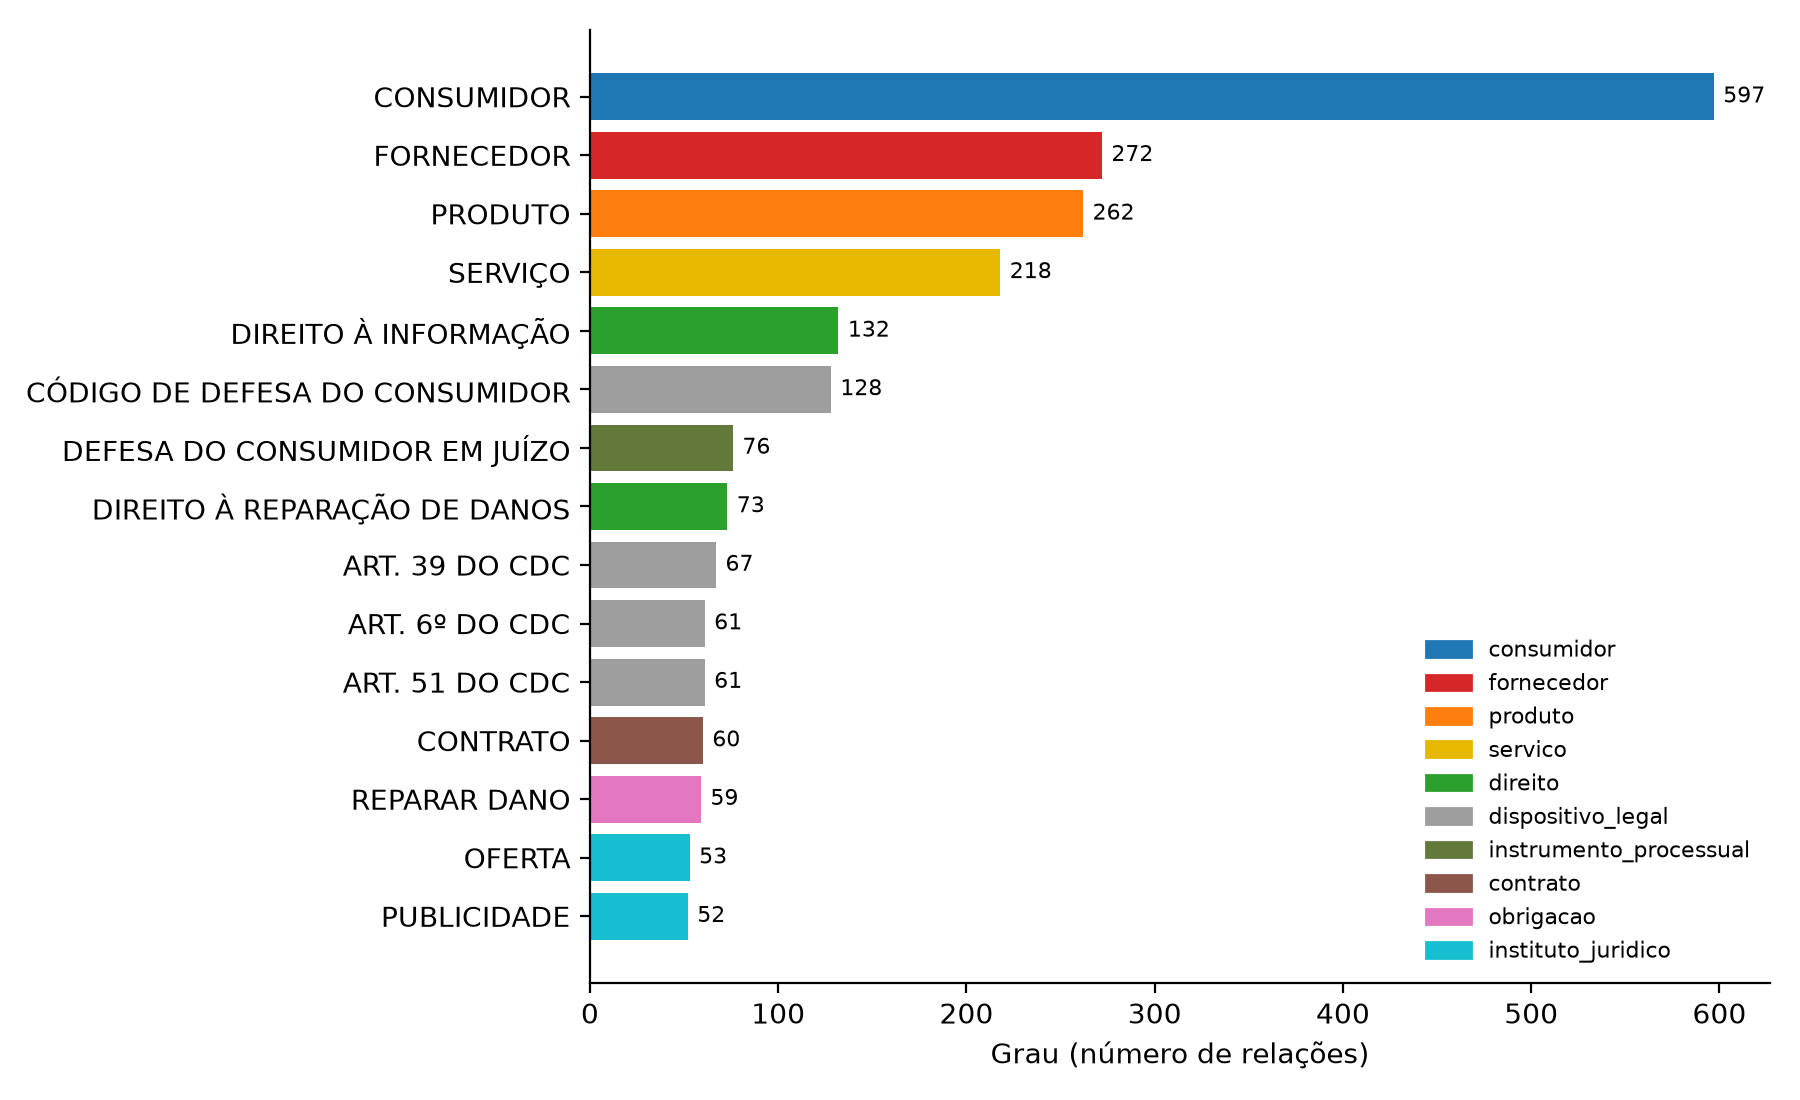
\includegraphics[width=.75\textwidth]{figuras/fig-grafo-graus.png}
\caption{As quinze entidades de maior grau do grafo do CDC, coloridas por tipo.}
\label{fig-grafo-graus}
\end{figure}

Essa concentração tem uma consequência para as buscas. Como as entidades centrais estão ligadas a quase tudo, elas aparecem no contexto de muitas consultas, mas acrescentam pouca informação específica; e, na busca local, as relações são ordenadas pelo grau combinado das entidades (Seção~\ref{sec-graphrag-indexacao-extracao}), o que favorece relações com as entidades centrais.

\subsection{Especialização em torno das entidades gerais}
\label{sec-analise-grafo-especializacao}

Filtrando o grafo na aplicação para exibir apenas os tipos consumidor, fornecedor, produto e serviço (Figura~\ref{fig-grafo-hubs}), observa-se uma estrutura que lembra a de uma hierarquia de classes: cada entidade geral é cercada por entidades menores que são casos particulares dela. A Figura~\ref{fig-grafo-especializacao} mostra essas estruturas em detalhe, considerando apenas as relações entre entidades do mesmo tipo.

\begin{figure}[htb]
\centering
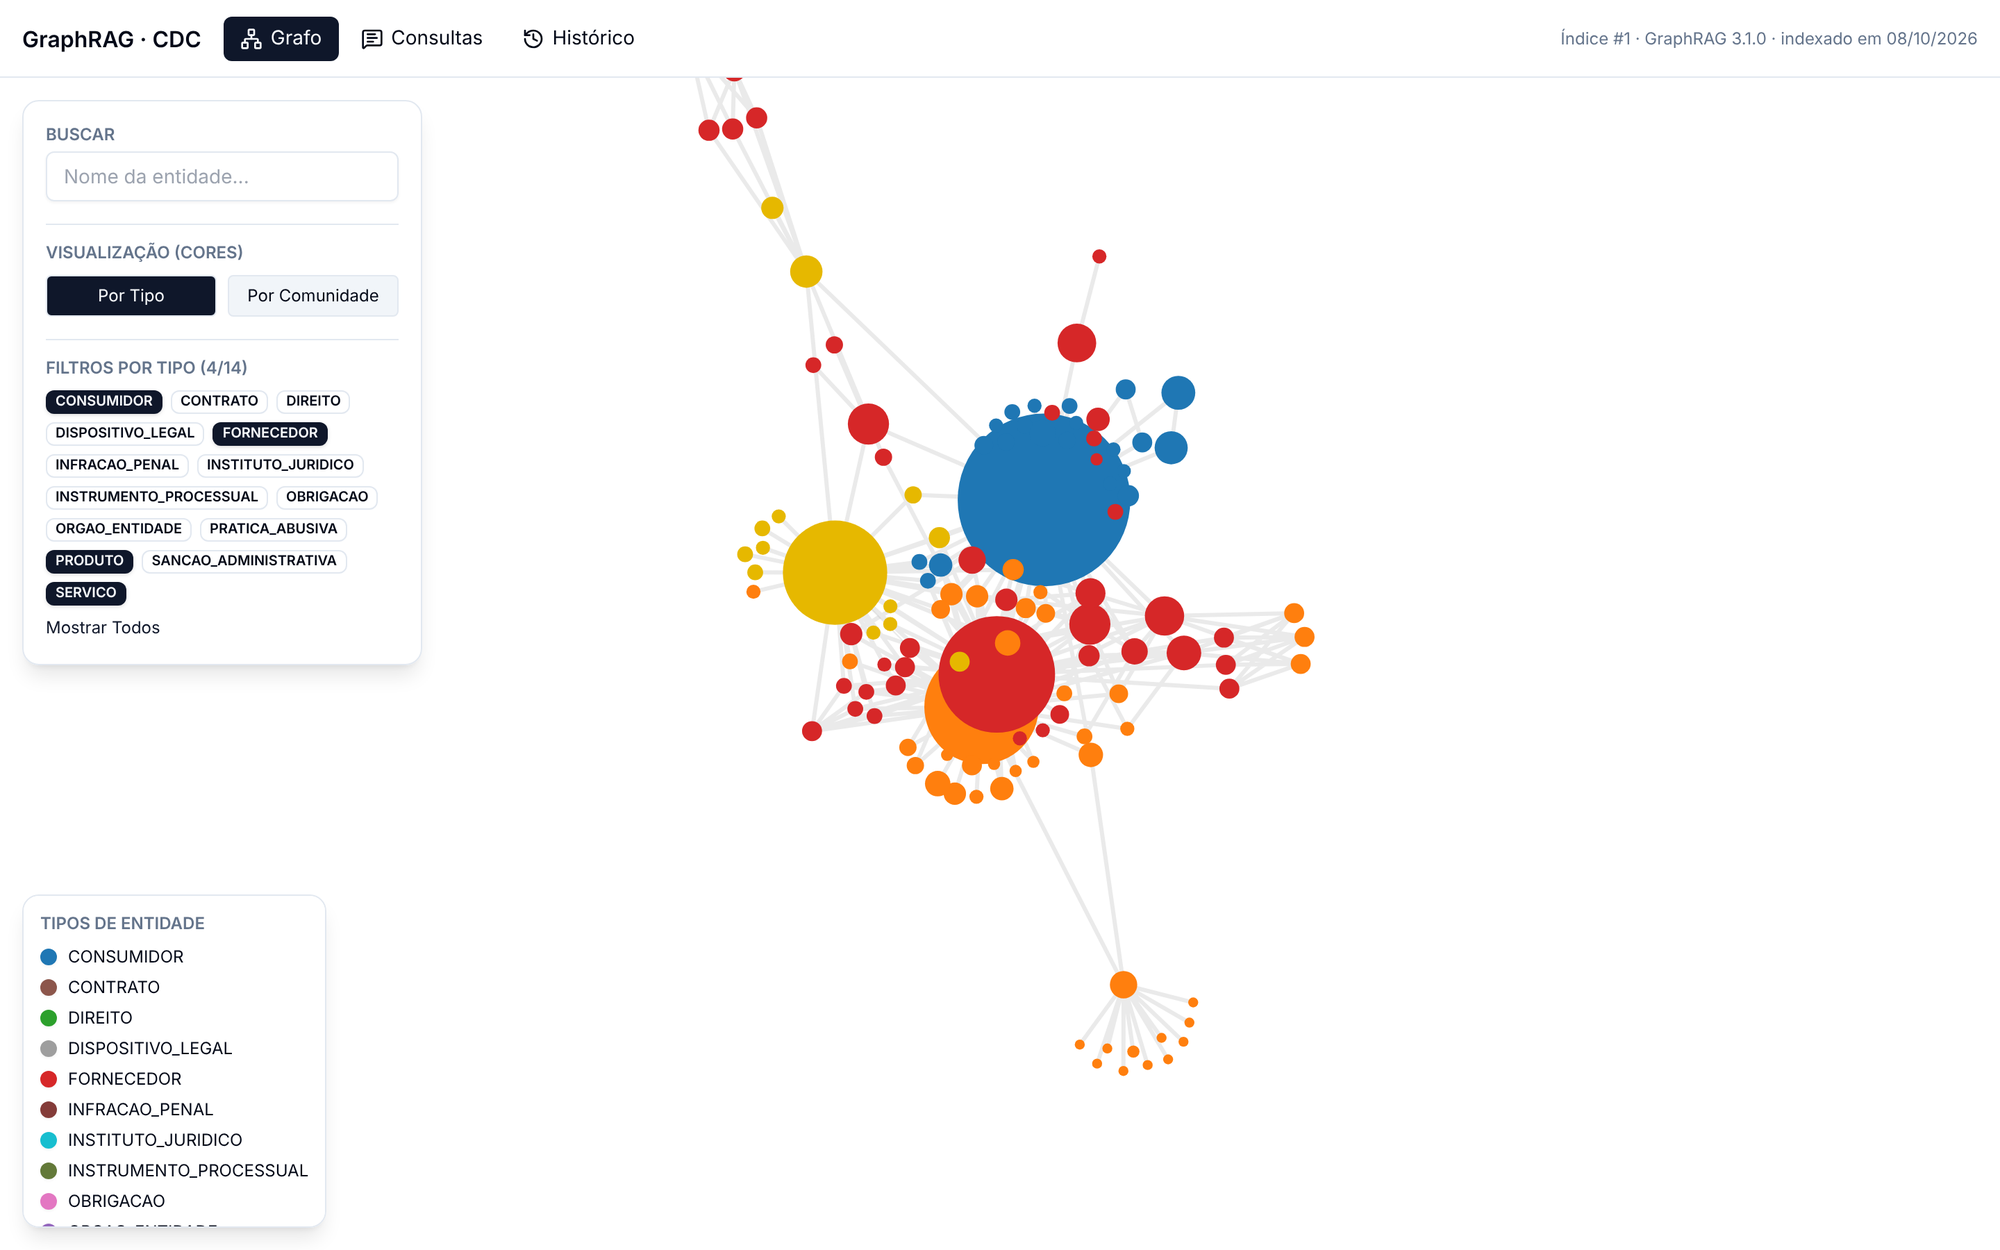
\includegraphics[width=.75\textwidth]{figuras/fig-grafo-hubs.png}
\caption{Aba Grafo filtrada para os tipos consumidor, fornecedor, produto e serviço: as quatro entidades gerais cercadas pelas entidades que as especializam.}
\label{fig-grafo-hubs}
\end{figure}

\begin{figure}[htbp]
\centering
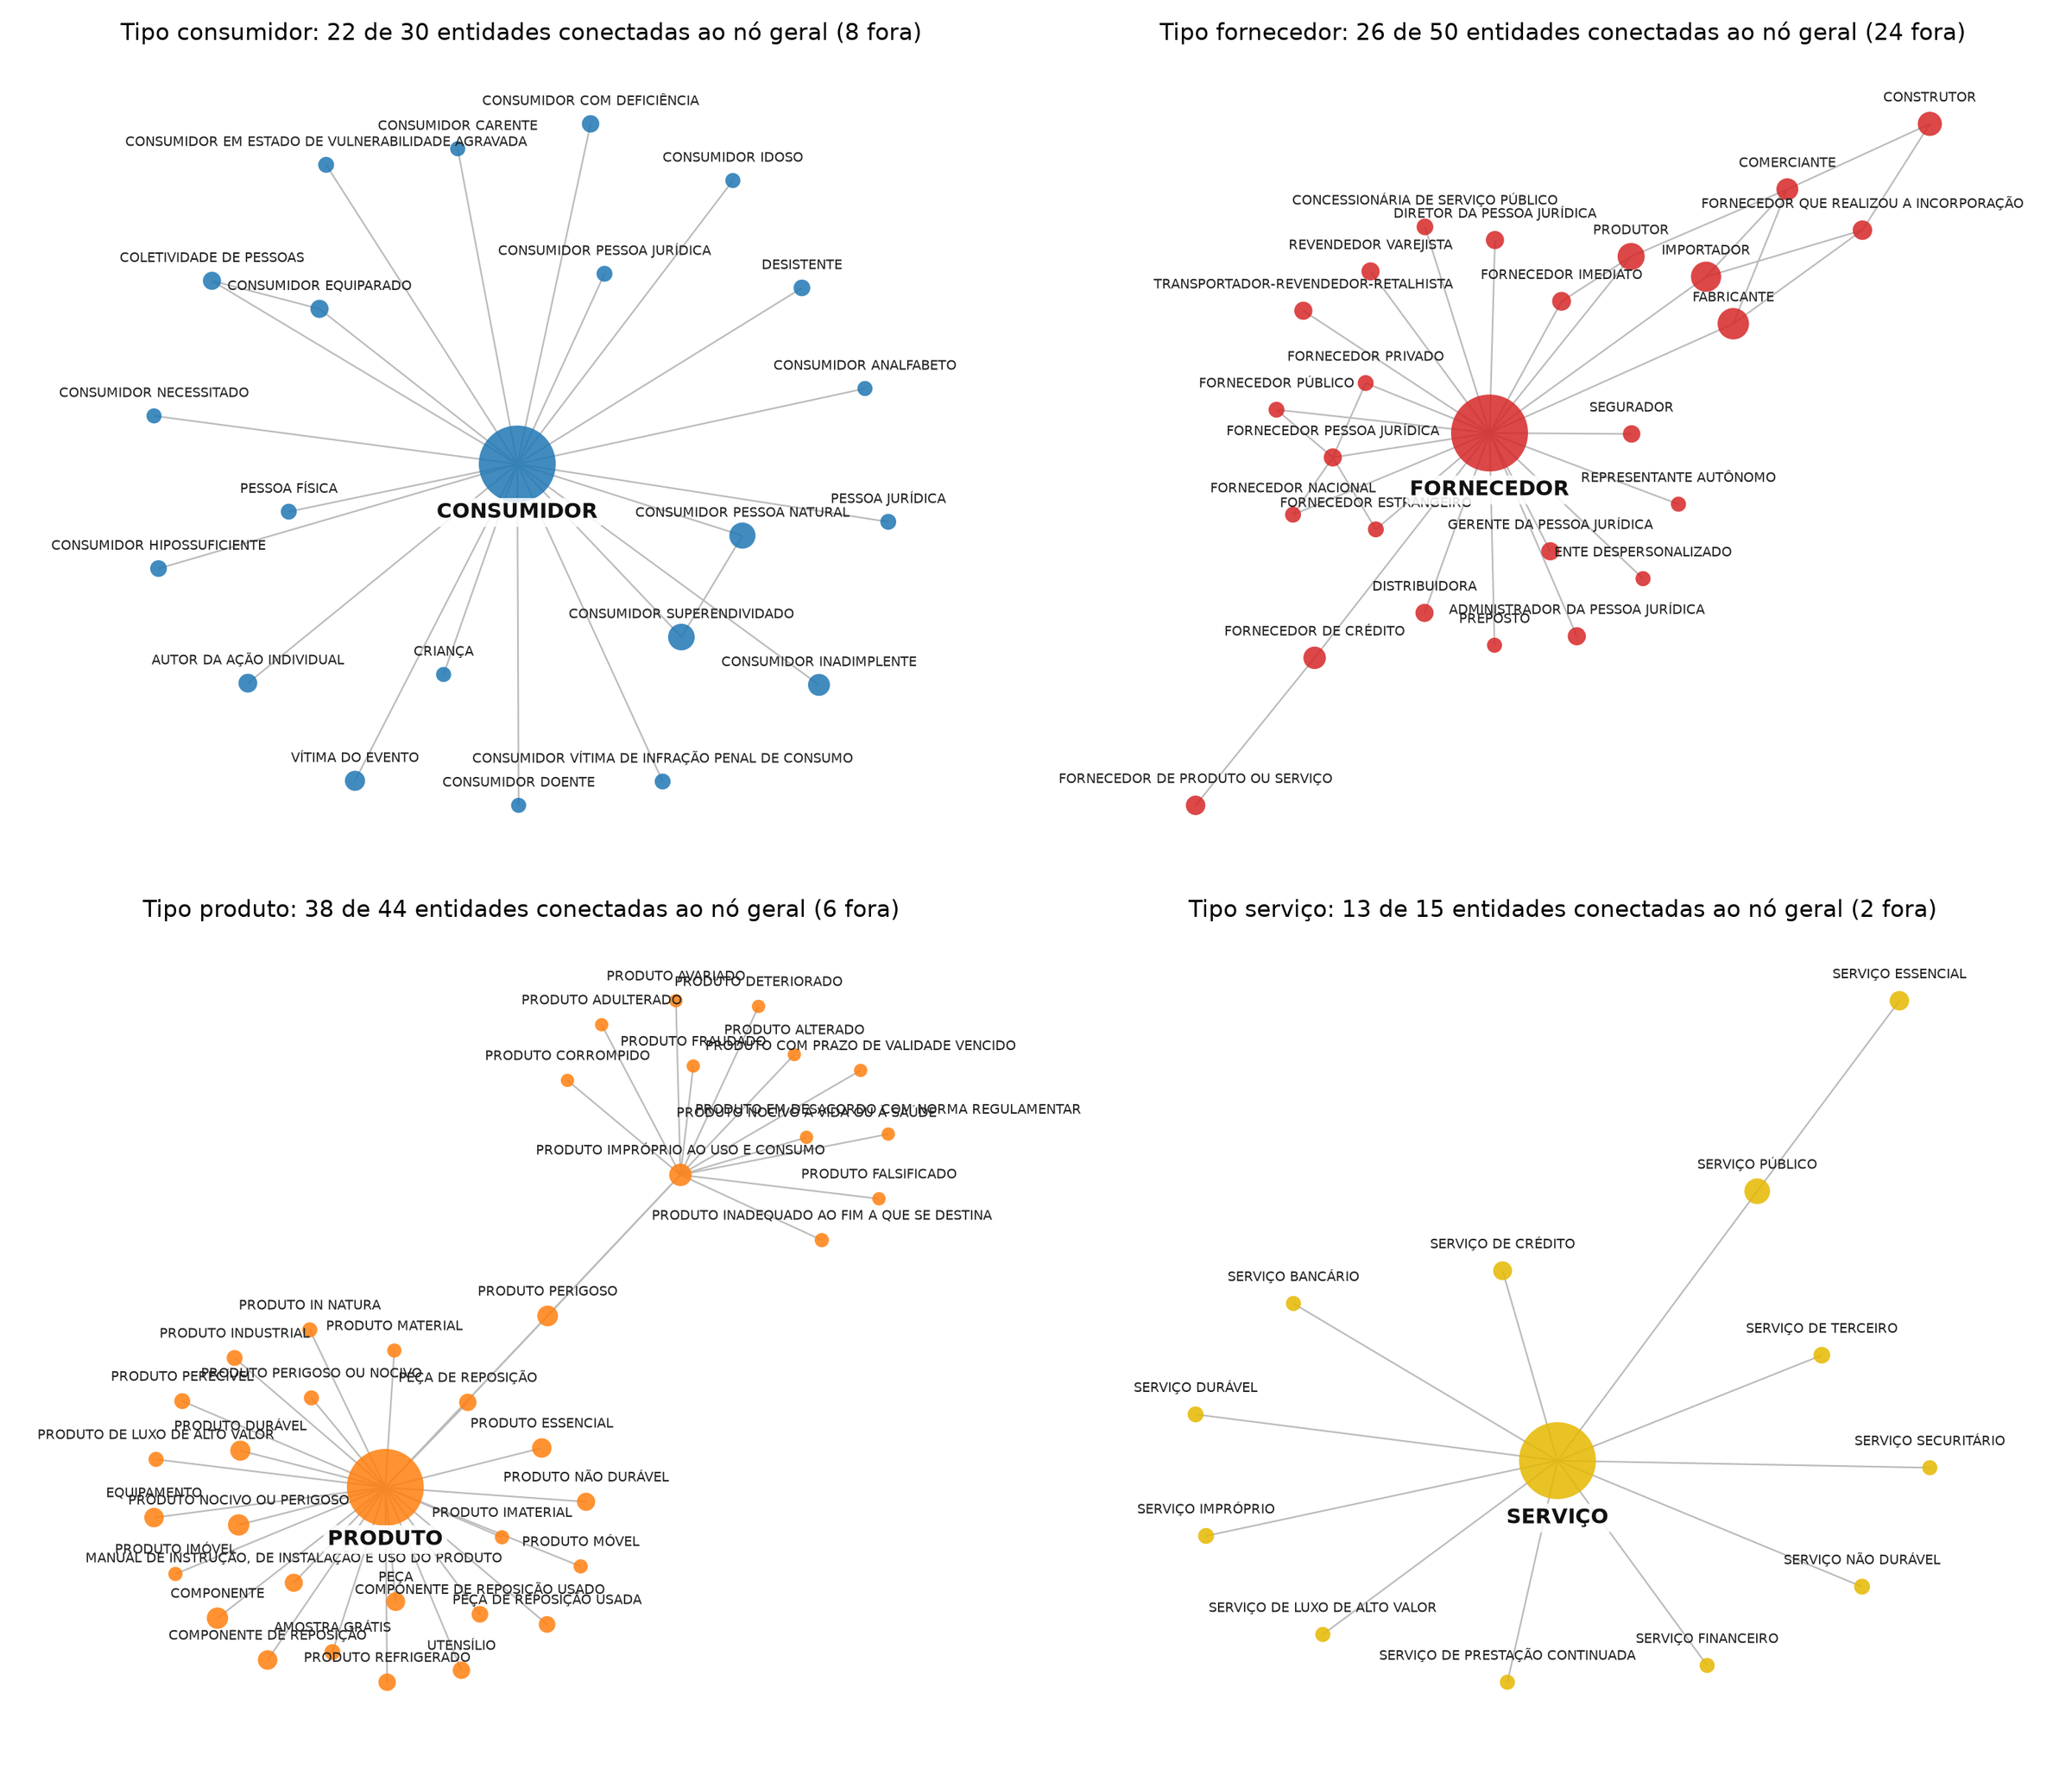
\includegraphics[width=.88\textwidth]{figuras/fig-grafo-especializacao.png}
\caption{Entidades de cada um dos tipos consumidor, fornecedor, produto e serviço e as relações entre elas. O tamanho dos nós é proporcional ao grau no grafo completo.}
\label{fig-grafo-especializacao}
\end{figure}

No tipo consumidor, a entidade geral CONSUMIDOR liga-se a especializações que correspondem a figuras previstas na lei -- CONSUMIDOR EQUIPARADO, COLETIVIDADE DE PESSOAS, VÍTIMA DO EVENTO, CONSUMIDOR SUPERENDIVIDADO -- e a situações de vulnerabilidade que o código protege de forma específica, como CONSUMIDOR IDOSO, CRIANÇA, CONSUMIDOR ANALFABETO e CONSUMIDOR COM DEFICIÊNCIA. No tipo fornecedor, FORNECEDOR liga-se às espécies enumeradas no art. 3º e nos artigos de responsabilidade -- FABRICANTE, PRODUTOR, CONSTRUTOR, IMPORTADOR, COMERCIANTE -- e a figuras introduzidas pelo tratamento do crédito, como FORNECEDOR DE CRÉDITO. O tipo produto apresenta dois níveis: PRODUTO é o centro de uma estrela (produto durável, não durável, perigoso, peça de reposição, amostra grátis), e PRODUTO IMPRÓPRIO AO USO E CONSUMO é o centro de outra, com as hipóteses do art. 18, § 6º (produto deteriorado, alterado, adulterado, avariado, falsificado, corrompido, fraudado, nocivo à vida ou à saúde, em desacordo com as normas regulamentares).

Essa estrutura não foi especificada em nenhum lugar: a taxonomia define apenas os tipos, e o \textit{prompt} de extração não pede relações de especialização. Ela emergiu da extração, porque o próprio texto da lei define os conceitos por gênero e espécie. Ao mesmo tempo, o grafo não distingue esse tipo de relação dos demais: a ligação entre CONSUMIDOR e CONSUMIDOR IDOSO é uma aresta como qualquer outra, com uma descrição em texto livre. Nem todas as especializações foram ligadas à entidade geral -- 8 das 30 entidades do tipo consumidor e 24 das 50 do tipo fornecedor não têm relação direta ou indireta com ela dentro do próprio tipo --, o que indica um limite da extração por trechos: a relação só é criada quando os dois conceitos aparecem no mesmo artigo.

\subsection{Relações, pesos e pontes entre artigos}
\label{sec-analise-grafo-relacoes}

As relações mais frequentes ligam dispositivos legais a institutos jurídicos (567 relações), a obrigações (280) e a direitos (257), o que reflete a forma como o grafo representa a lei: cada artigo é uma entidade ligada aos conceitos que ele trata. São também essas ligações que conectam artigos distantes no texto. A Figura~\ref{fig-grafo-ego} mostra a vizinhança da entidade DIREITO DE ARREPENDIMENTO: ela liga o art. 49, que cria o direito, ao art. 54-F, que, cinco capítulos adiante e incluído por outra lei, estende seus efeitos aos contratos de crédito conexos. No texto, nada aproxima os dois artigos além do assunto; no grafo, eles estão a dois passos de distância.

\begin{figure}[htb]
\centering
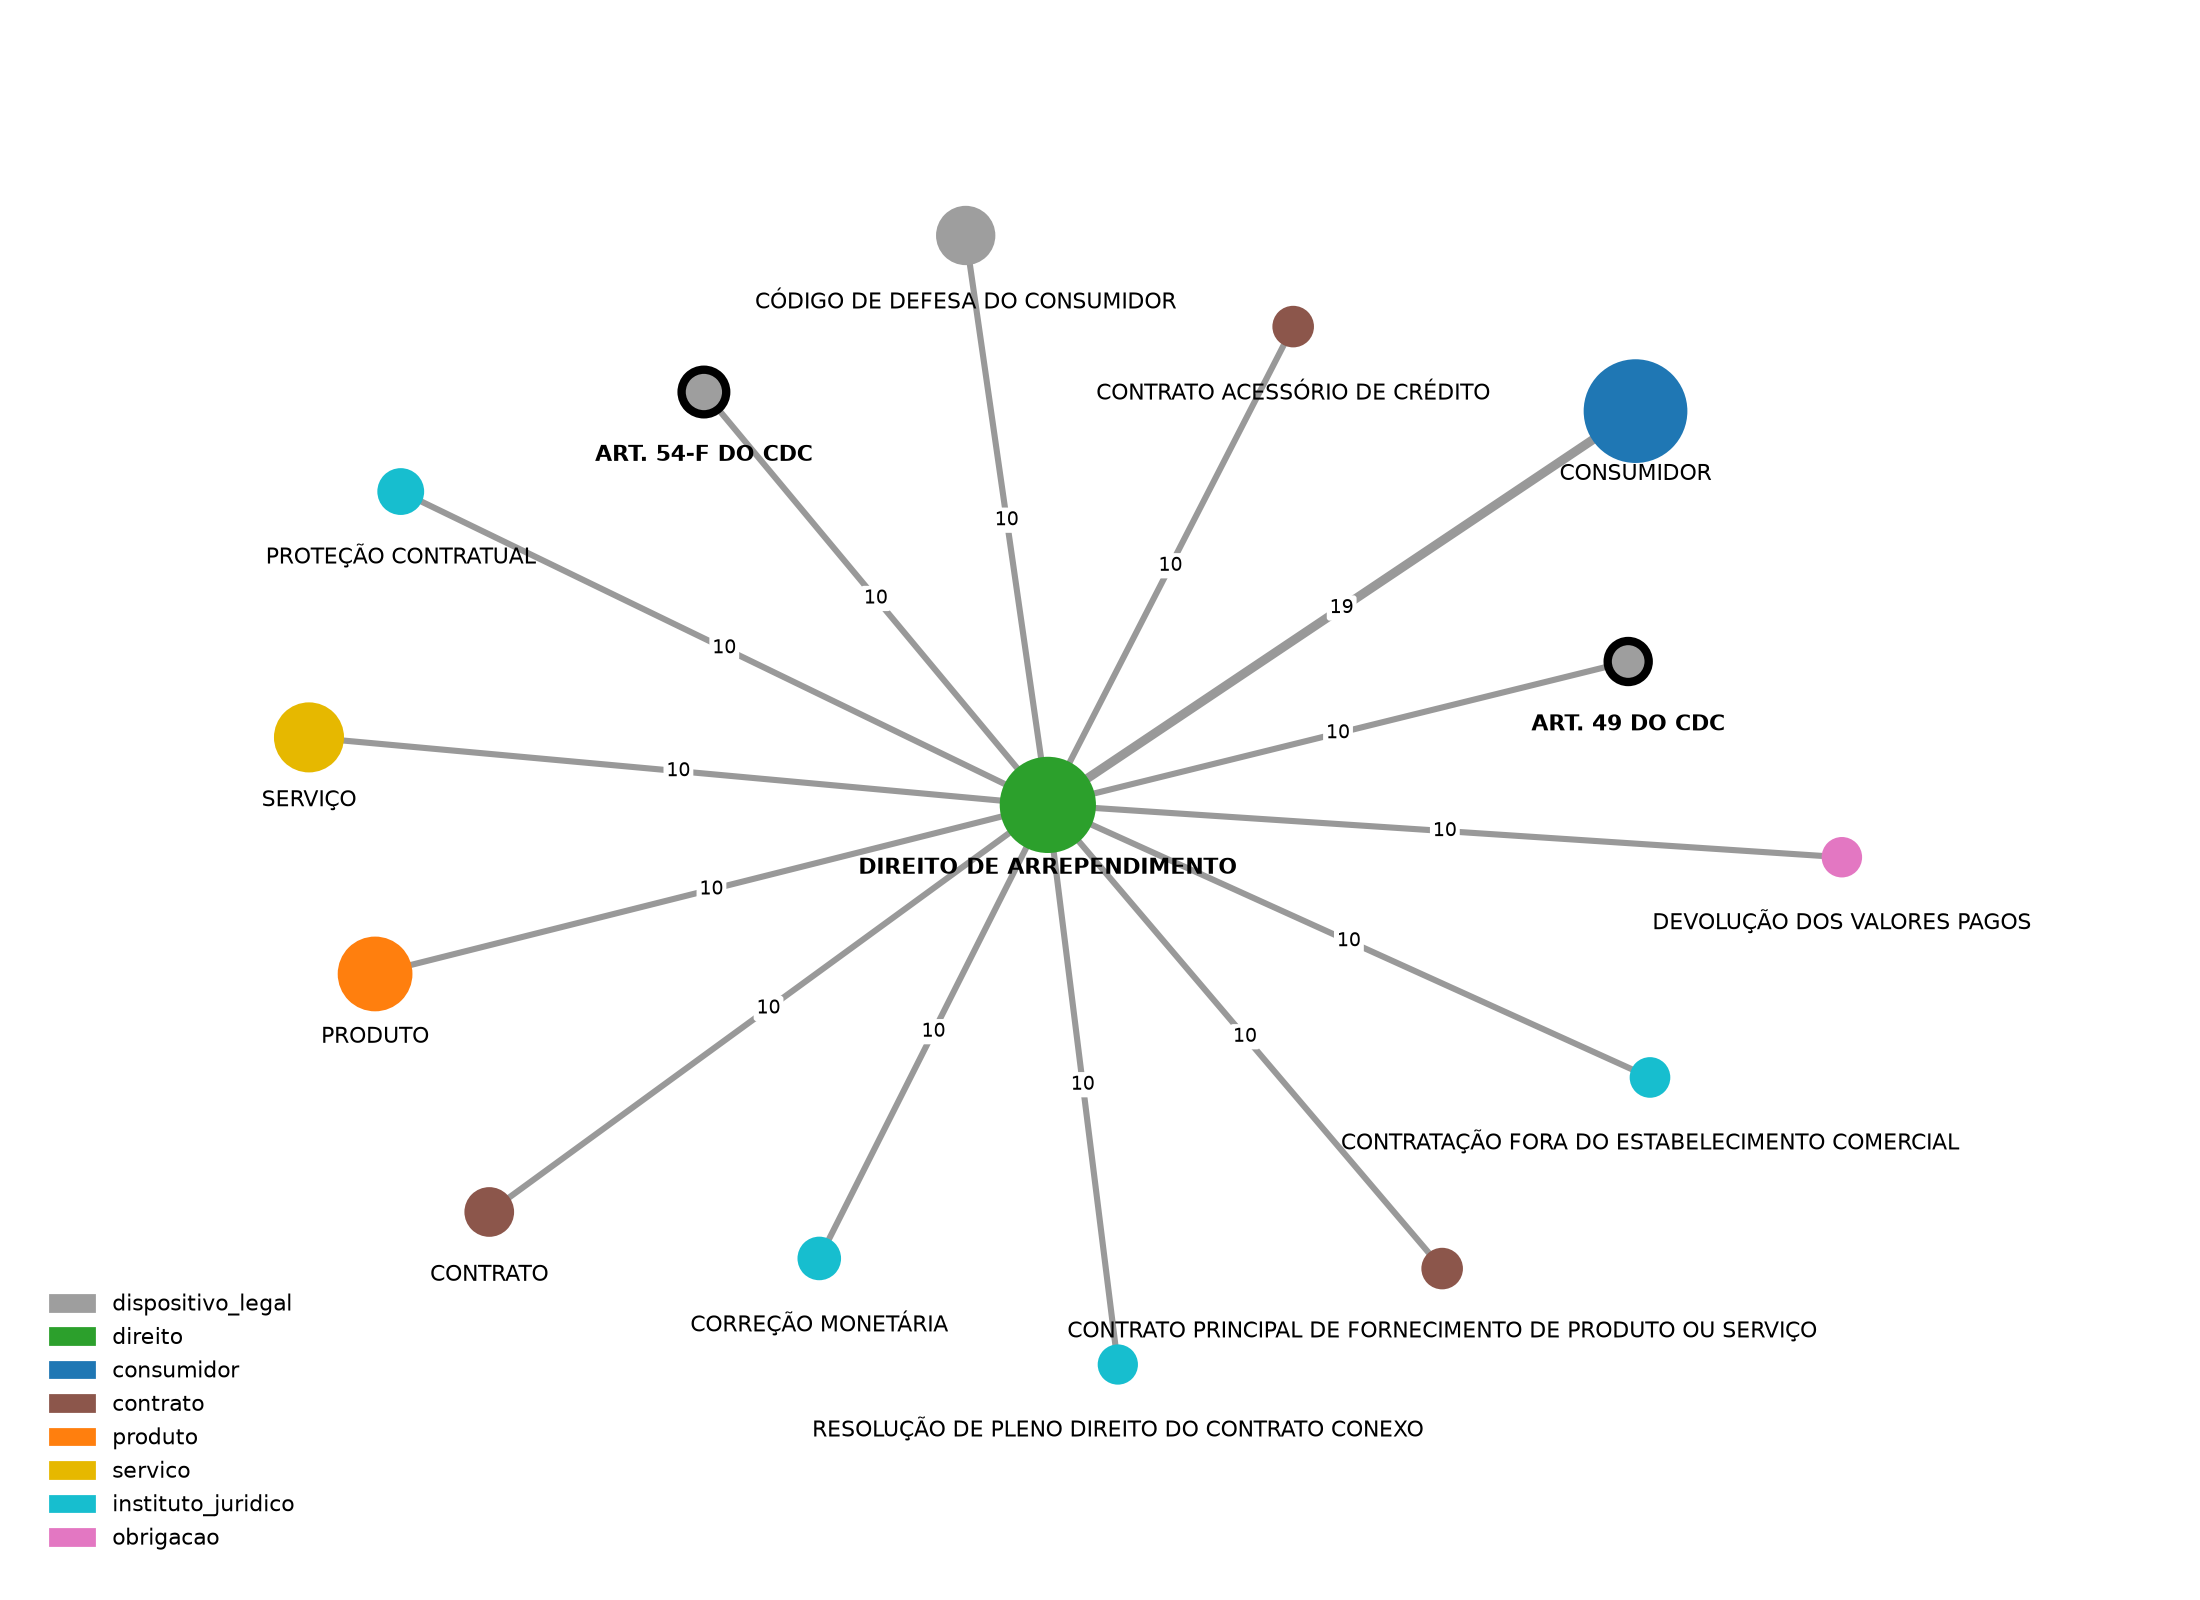
\includegraphics[width=.78\textwidth]{figuras/fig-grafo-ego-arrependimento.png}
\caption{Relações da entidade DIREITO DE ARREPENDIMENTO, com o peso de cada uma. Em destaque, os dois artigos que a mencionam.}
\label{fig-grafo-ego}
\end{figure}

A figura ilustra também como os pesos se comportam neste índice: quase todas as relações têm peso 10, a força máxima atribuída em uma única ocorrência, e a relação com CONSUMIDOR tem peso 19 porque aparece nos dois artigos. Como discutido na Seção~\ref{sec-graphrag-indexacao-extracao}, o peso funciona aqui, essencialmente, como uma contagem de ocorrências, e não como uma medida da intensidade da ligação.

Além dos artigos do CDC, o grafo representa as normas que o código menciona, e algumas delas funcionam como pontes entre partes distantes da lei: a LEI Nº 14.181/2021, que acrescentou o tratamento do superendividamento, liga os princípios e direitos básicos (arts. 4º a 6º) e os artigos sobre crédito do Título I (arts. 54-A a 54-G) aos artigos sobre a conciliação no superendividamento, no Título III (arts. 104-A a 104-C); e a LEI Nº 7.347/1985, da ação civil pública, liga as ações coletivas do Título III às disposições finais do Título VI, que alteram essa lei. Já a entidade CÓDIGO DE DEFESA DO CONSUMIDOR, com 128 relações com artigos e normas de todo o texto, funciona como um nó de ligação genérico, que pouco informa sobre o conteúdo.

\subsection{Comunidades}
\label{sec-analise-grafo-comunidades}

As comunidades do nível 0 (Tabela~\ref{tab-comunidades-n0} e Figura~\ref{fig-grafo-niveis}) correspondem a grandes temas do CDC -- tutela coletiva, superendividamento, sanções administrativas, tutela penal, vícios do produto, cadastros de consumidores --, mas não coincidem com a divisão formal da lei em títulos e capítulos. O direito de arrependimento, por exemplo, é criado no capítulo da proteção contratual, mas pertence, no nível 0, à comunidade do crédito ao consumidor, organizada em torno dos arts. 54-F e 54-G (Figura~\ref{fig-app-entidade}), o que reflete a ligação estabelecida pelo art. 54-F. O particionamento captura, portanto, uma organização temática transversal, que é a que interessa a quem pergunta sobre um assunto, e não sobre um capítulo. É essa organização que a busca global e o primer da DRIFT utilizam.

%%% Início de seção. %%%
\section{Roteiro de Análise das Consultas}
\label{sec-analise-roteiro}

Para cada consulta, a linha do tempo exibida pela aplicação (Seção~\ref{sec-aplicacao-frontend-consultas}) permite responder a um conjunto de perguntas sobre a recuperação:

\begin{enumerate}
    \item \textbf{O que foi recuperado?} As tabelas do contexto mostram, separadamente, as entidades, as relações, os relatórios de comunidade e os trechos de texto selecionados, com seus identificadores.
    \item \textbf{O que foi enviado ao modelo?} A etapa do \textit{prompt} mostra a mensagem de sistema final, com as instruções e o contexto já formatado, exatamente como o GraphRAG a monta, e o seu tamanho aproximado em \textit{tokens}.
    \item \textbf{Que parte do grafo esse contexto representa?} O subgrafo da consulta e o destaque no grafo completo mostram onde, no conhecimento extraído do CDC, o contexto se situa e quão concentrado ou disperso ele é.
    \item \textbf{O que a resposta usou do contexto?} As citações no formato \code{[Data: Sources (...)]} remetem aos identificadores das tabelas do contexto. Como cada unidade de texto corresponde a um artigo (Seção~\ref{sec-indexacao-segmentacao}), é possível saber quais artigos sustentam cada afirmação e quais artigos recuperados não foram usados.
    \item \textbf{Quanto custou?} As métricas mostram as chamadas ao modelo e os \textit{tokens} de entrada e saída, no total e por etapa.
\end{enumerate}

As seções a seguir aplicam esse roteiro a uma consulta de cada modalidade, na ordem crescente de complexidade.

%%% Início de seção. %%%
\section{Busca Básica: Recuperação por Similaridade}
\label{sec-analise-basic}

\textbf{Consulta:} ``O que acontece com o art. 54-E do CDC?'' -- 1 chamada, 4.452 \textit{tokens} de entrada, 123 de saída, 6,6 segundos.

\textbf{O que foi recuperado.} A busca básica recuperou as dez unidades de texto mais similares à pergunta (Figura~\ref{fig-app-contexto}, no Capítulo~\ref{sec-aplicacao}), correspondentes aos arts. 34, 53, 54, 54-B, 54-C, 54-D, 54-E, 54-F, 54-G e 85. O conjunto mostra como opera a similaridade vetorial: sete dos dez trechos pertencem ao capítulo do superendividamento, vizinhos do artigo pedido -- os metadados inseridos no início de cada trecho (Listagem~\ref{lst-chunk}), que repetem o nome do capítulo, contribuem para essa proximidade --, mas o art. 54-A, que abre o capítulo e define seus conceitos, não foi recuperado. O art. 85, de outro título, entrou por ser, como o 54-E, um artigo vetado cujo texto se resume à indicação do veto.

\textbf{O que foi enviado ao modelo.} Apenas texto: os dez trechos, com seus metadados, e as instruções. Um comportamento não documentado tornou-se visível aqui: a ordem dos trechos no \textit{prompt} é a ordem dos artigos no corpus, e não a ordem de similaridade. O código da busca básica converte os resultados da busca vetorial em um conjunto de identificadores e filtra a tabela de unidades de texto por esse conjunto, descartando o ranqueamento. Assim, o modelo não recebe nenhuma indicação de quais trechos são mais relevantes (defeito 12 da Tabela~\ref{tab-defeitos}).

\textbf{Que parte do grafo.} Embora a busca básica não use o grafo, o destaque mostra as entidades extraídas dos mesmos trechos: 160 entidades, espalhadas sobretudo pela região do grafo ligada ao crédito e ao superendividamento. Esse número contrasta com o que o modelo recebeu -- dez trechos de texto, sem nenhuma das relações que o grafo conhece entre eles.

\textbf{O que a resposta usou.} A resposta afirmou corretamente que o artigo foi vetado, que aparece no texto apenas como ``Art. 54-E. (VETADO)'' e que está associado à Lei nº 14.181/2021 e ao capítulo do superendividamento, citando apenas a unidade de texto do próprio artigo. O modelo ressalvou que os dados não informam a redação proposta nem os motivos do veto, comportamento desejável diante de um contexto que, de fato, não continha essa informação. Os outros nove trechos não foram utilizados. A resposta só foi possível porque o texto vetado foi mantido no corpus (Seção~\ref{sec-indexacao-corpus-vetados}).

%%% Início de seção. %%%
\section{Busca Local: Contexto a Partir das Entidades}
\label{sec-analise-local}

\textbf{Consulta:} ``O que diz o art. 49 do CDC sobre o direito de arrependimento?'' -- 1 chamada, 10.154 \textit{tokens} de entrada, 205 de saída, 8,6 segundos.

\textbf{O que foi recuperado.} O contexto da busca local é estruturado em tabelas:

\begin{itemize}
    \item \textbf{20 entidades}, selecionadas por similaridade entre a pergunta e as descrições: ``ART. 49 DO CDC'', ``DIREITO DE ARREPENDIMENTO'', ``DEVOLUÇÃO DOS VALORES PAGOS'', ``CONTRATAÇÃO FORA DO ESTABELECIMENTO COMERCIAL'', direitos relacionados ao desfazimento de contratos (reembolso da quantia paga, rescisão do contrato, desfazimento do negócio, cumprimento das declarações de vontade) e doze outros artigos (18, 19, 20, 24, 26, 35, 39, 46, 47, 48, 50 e 53);
    \item \textbf{9 relações}, todas partindo de ``ART. 49 DO CDC'': com CONSUMIDOR, PRODUTO, SERVIÇO, CONTRATO, PROTEÇÃO CONTRATUAL, CORREÇÃO MONETÁRIA, DIREITO DE ARREPENDIMENTO, CONTRATAÇÃO FORA DO ESTABELECIMENTO COMERCIAL e DEVOLUÇÃO DOS VALORES PAGOS;
    \item \textbf{17 trechos de texto}, os artigos de onde essas entidades foram extraídas: 49 em primeiro lugar, seguido do 54-F (contratos conexos, que também tratam do arrependimento), dos artigos vizinhos da proteção contratual (46, 47, 48, 50, 51, 53 e 54) e de artigos sobre vícios, oferta e práticas abusivas (18, 19, 20, 24, 26, 35, 39 e 41);
    \item \textbf{nenhum relatório de comunidade}.
\end{itemize}

A ausência de relatórios foi outro achado que a ferramenta tornou visível. Com os valores padrão, a busca local reserva 15\% do contexto (1.800 \textit{tokens}) para os relatórios de comunidade, e todos os relatórios deste índice são maiores que isso: o menor tem cerca de 1.300 \textit{tokens}, e a mediana, cerca de 2.300. Como a montagem do contexto não trunca relatórios, nenhum é incluído (defeito 13 da Tabela~\ref{tab-defeitos}). Ou seja, com a configuração padrão e relatórios do tamanho gerado neste trabalho, a busca local usa entidades, relações e trechos, mas não a visão de comunidade.

\textbf{O que foi enviado ao modelo.} Cerca de nove mil \textit{tokens} de contexto e instruções (Figura~\ref{fig-analise-prompt}), mais que o dobro da busca básica, organizados em tabelas com identificadores que o modelo deve citar.

\begin{figure}[htbp]
\centering
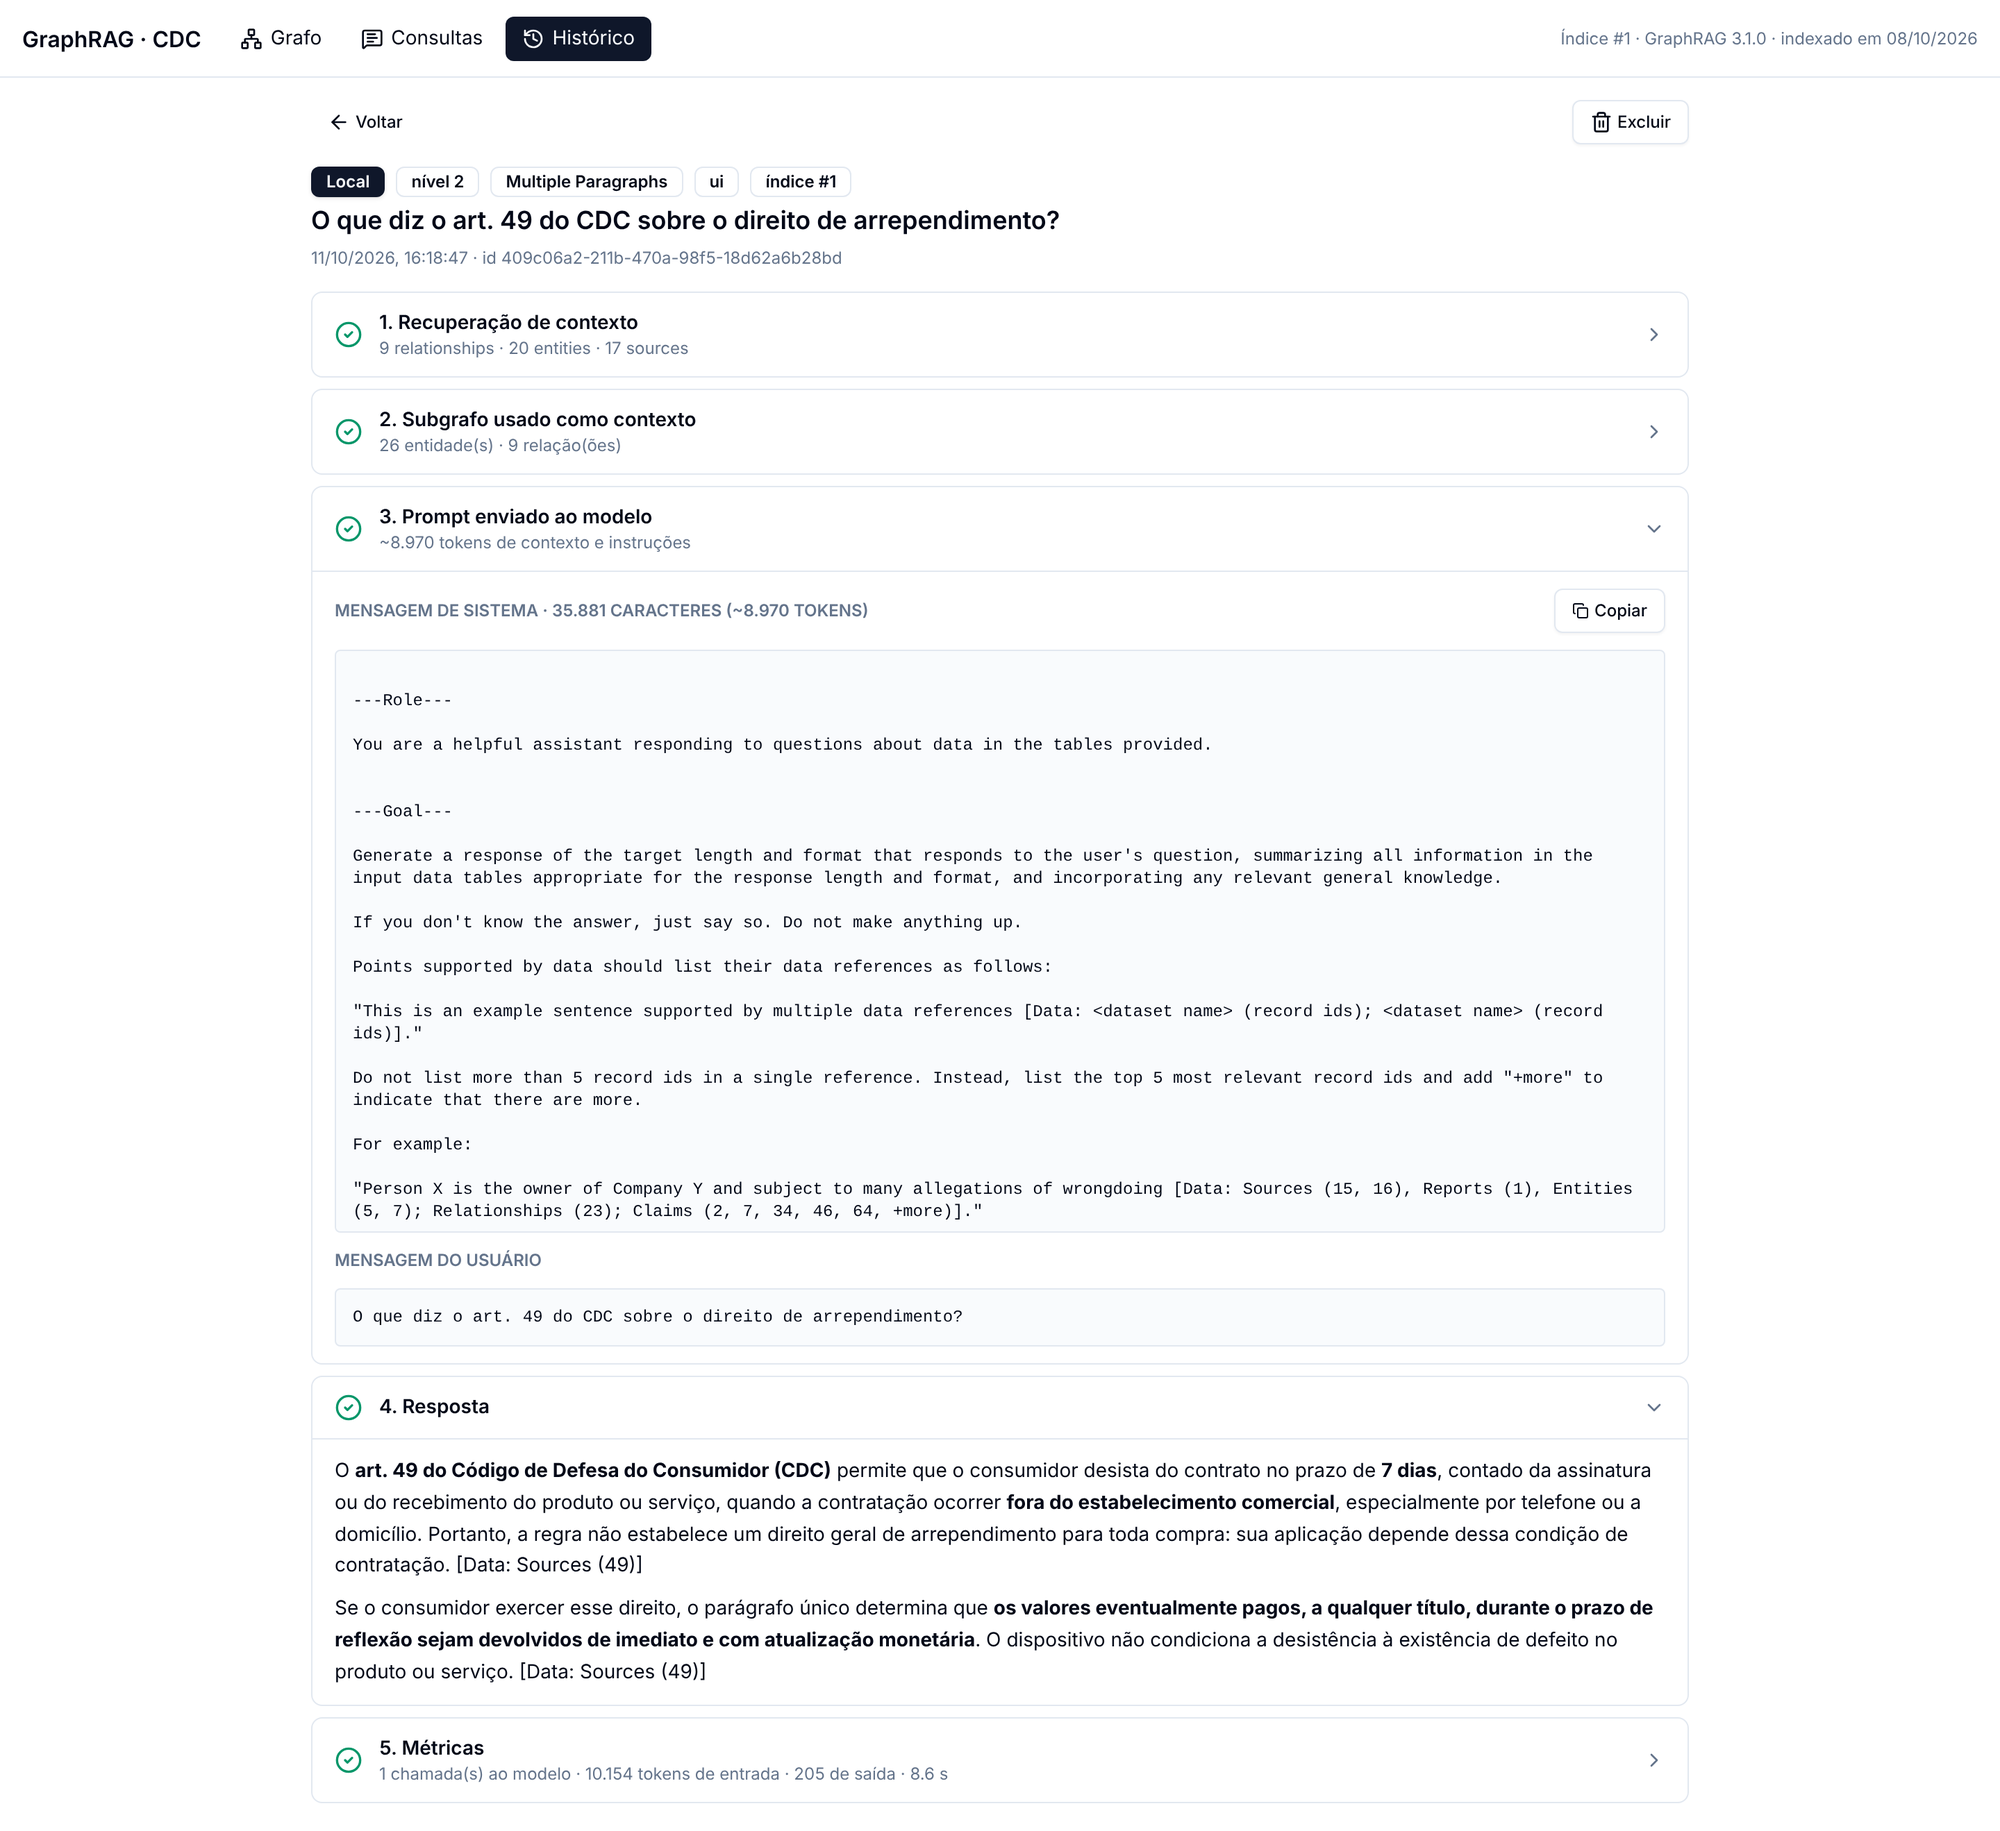
\includegraphics[width=.7\textwidth]{figuras/fig-app-local-prompt.png}
\caption{Etapa do \textit{prompt} enviado ao modelo na consulta da busca local sobre o art. 49: instruções seguidas das tabelas de entidades, relações e trechos.}
\label{fig-analise-prompt}
\end{figure}

\textbf{Que parte do grafo.} O destaque (Figura~\ref{fig-app-destaque}, no Capítulo~\ref{sec-aplicacao}) mostra um contexto concentrado: 26 entidades -- as 20 da tabela e 6 que só aparecem como extremidade das relações, como CONSUMIDOR e PRODUTO -- e 9 relações, formando uma estrela em torno do art. 49, cercada pelos artigos vizinhos da proteção contratual e pelos artigos sobre vícios. É a vizinhança do artigo no grafo, e não apenas os trechos de vocabulário parecido.

\textbf{O que a resposta usou.} A resposta descreveu corretamente o prazo de sete dias, a condição de contratação fora do estabelecimento comercial e a devolução imediata e atualizada dos valores pagos, ressaltando que a regra não cria um direito geral de arrependimento para toda compra, e citou apenas a unidade de texto do art. 49. O contexto oferecia conexões que a resposta não explorou, como a extensão do arrependimento aos contratos conexos prevista no art. 54-F. Para uma pergunta pontual sobre o conteúdo de um artigo, isso é adequado. Mas o exemplo mostra que um contexto mais rico não se traduz automaticamente em uma resposta mais rica: o que o modelo usa depende também da pergunta e das instruções do \textit{prompt}.

%%% Início de seção. %%%
\section{Busca DRIFT: Exploração Iterativa}
\label{sec-analise-drift}

\textbf{Consulta:} ``Quais são os direitos básicos do consumidor?'' -- configuração padrão, nível de comunidade 2; 67 chamadas, 524.646 \textit{tokens} de entrada, 62.925 de saída, 221 segundos.

\textbf{O que foi recuperado.} A DRIFT é a modalidade em que a inspeção das etapas mais revela, porque ela própria decide o que pesquisar. As etapas registradas mostram:

\begin{itemize}
    \item \textbf{Primer}: os 20 relatórios de comunidade mais similares à resposta hipotética foram divididos em cinco grupos; cada grupo produziu uma resposta parcial -- todas centradas no art. 6º -- e uma lista de perguntas de acompanhamento. Foram geradas 28 perguntas, como ``Quais informações o fornecedor deve apresentar sobre produtos e serviços?'', ``Quando uma cláusula contratual é considerada abusiva pelo CDC?'' e ``Quais são os prazos para reclamar de vícios em produtos?''.
    \item \textbf{Aprofundamento}: em três rodadas, 60 perguntas foram respondidas, cada uma por uma busca local completa, e cada resposta gerou novas perguntas. A Tabela~\ref{tab-drift-arvore} mostra a árvore resultante: 502 perguntas, das quais 61 respondidas (incluindo a original). As perguntas se afastam da original à medida que a árvore se aprofunda: no terceiro nível aparecem perguntas como ``Quais são as penas pela omissão de advertências sobre riscos?'' e ``Como registrar uma reclamação no Procon ou ingressar no Juizado Especial Cível?''.
    \item \textbf{Contexto das buscas locais}: nas 60 buscas locais, o contexto continha \textbf{apenas trechos de texto} -- nenhuma entidade, relação ou relatório (defeito 7 da Tabela~\ref{tab-defeitos}). Somadas, as buscas recuperaram 1.189 trechos, com muitas repetições, cobrindo 116 dos 130 artigos do CDC; os mais frequentes foram os arts. 18 (36 vezes), 35, 20, 6º, 19 e 51.
    \item \textbf{Redução}: as 61 respostas parciais, cerca de 49 mil \textit{tokens}, foram enviadas a uma chamada final.
\end{itemize}

\begin{table}[htb]
\centering
\caption{Árvore de perguntas da consulta DRIFT, por profundidade.}
\label{tab-drift-arvore}
\footnotesize
\begin{tabular}{L{6cm} r r r}
\toprule
\textbf{Profundidade} & \textbf{Perguntas geradas} & \textbf{Respondidas} & \textbf{Não respondidas} \\
\midrule
0 (pergunta original) & 1 & 1 & 0 \\
1 (geradas pelo primer) & 28 & 21 & 7 \\
2 & 176 & 30 & 146 \\
3 & 234 & 9 & 225 \\
4 & 63 & 0 & 63 \\
\midrule
\textbf{Total} & \textbf{502} & \textbf{61} & \textbf{441} \\
\bottomrule
\end{tabular}
\end{table}

\textbf{Que parte do grafo.} Com a configuração padrão, a DRIFT usa o grafo apenas no primer, por meio dos relatórios de comunidade; o aprofundamento é, na prática, uma sequência de buscas por trechos de texto guiada por perguntas geradas pelo modelo. Por isso, o subgrafo exibido pela aplicação para essa consulta é vazio. Esse resultado não seria perceptível pela resposta, que é extensa e correta, nem pelas métricas: só a inspeção do contexto de cada busca local o revelou.

\textbf{O que a resposta usou.} A resposta final organizou os direitos básicos do art. 6º em grupos temáticos (segurança, educação e informação; proteção contra abusos e equilíbrio contratual; reparação de danos e acesso à defesa; serviços públicos e proteção financeira) e acrescentou outros direitos relevantes na prática, como a garantia legal e o direito de arrependimento. As citações remetem ao art. 6º e, no último bloco, aos arts. 18, 20, 24, 30 e 49. Ou seja, das dezenas de artigos explorados, poucos chegaram à resposta, o que é esperado em uma síntese, mas indica que boa parte do custo da exploração não se refletiu no resultado.

\textbf{Quanto custou.} A etapa de aprofundamento respondeu por 417 mil dos 525 mil \textit{tokens} de entrada (cerca de sete mil por busca local), o primer por 56 mil e a redução por 49 mil. A consulta custou, em \textit{tokens} de entrada, cerca de cinquenta vezes a busca local. A análise das opções de configuração da DRIFT (Seção~\ref{sec-graphrag-config-consultas}) mostra que é possível reduzir esse custo diminuindo o número de perguntas por rodada e de rodadas, e fazer as buscas locais usarem o grafo ajustando as proporções de contexto.

%%% Início de seção. %%%
\section{Busca Global: Síntese a Partir das Comunidades}
\label{sec-analise-global}

Na busca global, a ferramenta exibe as etapas do \textit{map-reduce}: os relatórios de comunidade considerados, os lotes enviados ao modelo, os pontos-chave de cada lote ordenados pela nota de importância e com o lote de origem, o \textit{prompt} da síntese e a resposta final. O destaque no grafo mostra as comunidades cujos relatórios foram efetivamente citados nos pontos-chave relevantes e na resposta, o que permite distinguir as comunidades lidas das comunidades usadas.

Nesta versão do trabalho, a busca global foi exercitada com o índice real e com os modelos simulados da biblioteca, o que permitiu medir o tamanho do contexto em cada nível da hierarquia sem custo de geração (Tabela~\ref{tab-global-niveis}). Os números mostram que, para a busca global, o nível de comunidade é a principal decisão de análise: no nível 0, o modelo lê 17 relatórios amplos, que correspondem aos grandes temas do CDC (Tabela~\ref{tab-comunidades-n0}); nos níveis mais profundos, lê centenas de relatórios específicos, com custo mais de dez vezes maior. A análise qualitativa de consultas globais reais, nos diferentes níveis, fica como trabalho futuro.

\begin{table}[htb]
\centering
\caption{Tamanho do contexto da busca global por nível de comunidade, medido no índice do CDC.}
\label{tab-global-niveis}
\footnotesize
\begin{tabular}{L{4cm} r r}
\toprule
\textbf{Nível de comunidade} & \textbf{Chamadas ao modelo} & \textbf{\textit{Tokens} de entrada} \\
\midrule
0 & 7 & 71 mil \\
1 & 30 & 336 mil \\
2 (padrão) & 68 & 775 mil \\
3 & 82 & 944 mil \\
\bottomrule
\end{tabular}
\end{table}

%%% Início de seção. %%%
\section{Síntese}
\label{sec-analise-sintese}

A Tabela~\ref{tab-analise-sintese} resume o que a ferramenta mostrou sobre o contexto de cada modalidade nas consultas analisadas.

\begin{table}[htb]
\centering
\caption{Síntese do contexto enviado ao modelo em cada modalidade, nas consultas analisadas.}
\label{tab-analise-sintese}
\footnotesize
\begin{tabular}{L{1.5cm} L{4.4cm} L{3.2cm} L{4.8cm}}
\toprule
\textbf{Busca} & \textbf{Contexto enviado ao modelo} & \textbf{Chamadas / \textit{tokens} de entrada} & \textbf{O que a inspeção revelou} \\
\midrule
Básica & 10 trechos, sem estrutura & 1 / 4,5 mil & Trechos vizinhos ao artigo pedido; ordem de similaridade descartada; artigo central do capítulo não recuperado \\
Local & 20 entidades, 9 relações e 17 trechos em tabelas & 1 / 10 mil & Vizinhança do artigo no grafo; nenhum relatório de comunidade por falta de espaço; resposta usou só o artigo central \\
DRIFT & Relatórios (primer); 60 contextos só com trechos; 61 respostas parciais (redução) & 67 / 525 mil & Grafo usado só no primer; cobertura de 116 artigos; perguntas cada vez mais distantes da original; custo concentrado no aprofundamento \\
Global & Lotes de relatórios de comunidade & 7 a 82 / 71 a 944 mil (por nível) & Custo determinado pelo nível de comunidade \\
\bottomrule
\end{tabular}
\end{table}

Três observações gerais emergem desses exemplos. A primeira é que as modalidades diferem muito mais no que enviam ao modelo do que se percebe pelas respostas: as três respostas analisadas são corretas, mas se apoiam em contextos de natureza, tamanho e custo muito diferentes. A segunda é que a configuração padrão do GraphRAG, combinada às características do índice -- em particular, relatórios de comunidade maiores que o espaço reservado a eles --, faz com que partes da estrutura de grafo simplesmente não cheguem ao modelo na busca local e na DRIFT, sem nenhum aviso. A terceira é que esses comportamentos só puderam ser identificados porque a aplicação expõe, para cada consulta, o contexto e o \textit{prompt} efetivamente utilizados. Essa é a principal contribuição da prova de conceito como ferramenta: tornar a recuperação observável, o que é condição para qualquer comparação criteriosa entre as modalidades.

% ==============================================================================
% Monografia - Áurea Santos de Oliveira
% Capítulo 7 - Considerações Finais
% ==============================================================================
\chapter{Conclusão}
\label{sec-conclusoes}

\aluno{Capítulo a ser concluído após a avaliação. Os pontos abaixo são um rascunho com o que já pode ser afirmado sobre o desenvolvimento.}

%%% Início de seção. %%%
\section{Considerações Finais}
\label{sec-conclusoes-consideracoes}

Este trabalho aplicou o \textit{framework} GraphRAG ao Código de Defesa do Consumidor, construindo uma prova de conceito que compreende a estruturação do texto da lei, a indexação em grafo de conhecimento e uma aplicação web para exploração do grafo e realização de consultas nas quatro modalidades da ferramenta, com registro detalhado de cada etapa.

Algumas lições do desenvolvimento já podem ser registradas:

\begin{itemize}
    \item \textbf{A preparação do corpus importa.} Estruturar a lei em um registro por artigo, com a hierarquia e a situação normativa inseridas em cada trecho, fez com que cada unidade de texto correspondesse a um artigo completo e permitiu que o grafo registrasse corretamente localização, vetos e revogações.
    \item \textbf{A qualidade do grafo depende da padronização.} Como o GraphRAG funde entidades pelo nome e pelo tipo, as definições dos tipos e as regras de nomeação inseridas no \textit{prompt} de extração foram decisivas para evitar nós duplicados.
    \item \textbf{O custo é dominado pela extração e pelas modalidades com muitas chamadas.} A indexação custou várias vezes a estimativa feita a partir do tamanho do corpus, e as buscas global e DRIFT custam dezenas de vezes uma busca local, conforme a configuração.
    \item \textbf{Usar a biblioteca exige ler o código.} Defeitos e comportamentos não documentados -- como a busca básica que devolve resposta vazia quando usada programaticamente, as buscas locais da DRIFT que não usam o grafo com a configuração padrão e o ajuste de \textit{prompts} que gera todos os exemplos a partir do mesmo trecho -- afetam diretamente a comparação entre as modalidades e só foram identificados pela inspeção do código e dos dados intermediários. A aplicação desenvolvida, ao expor cada etapa das consultas, foi o que tornou possível identificá-los.
\end{itemize}

\pendente{[Relacionar os resultados da avaliação aos objetivos da Seção~\ref{sec-intro-obj}; limitações; dificuldades; experiência adquirida.]}

%%% Início de seção. %%%
\section{Trabalhos Futuros}
\label{sec-conclusoes-trabalhosfuturos}

\pendente{[Rascunho de possibilidades:]}

\begin{itemize}
    \item ampliar o corpus com outras leis relacionadas (por exemplo, a Lei da Ação Civil Pública e regulamentações do CDC) e com jurisprudência, aproveitando o \textit{parser} genérico e as remissões entre normas já representadas no grafo;
    \item explorar a extração de alegações (\textit{claims}) e a seleção dinâmica de comunidades;
    \item comparar provedores e modelos de linguagem, inclusive modelos locais, mantendo o restante da configuração;
    \item reportar à equipe do GraphRAG os defeitos identificados, com as correções propostas;
    \item avaliar automaticamente as respostas com um LLM como juiz, comparando com a avaliação manual.
\end{itemize}




%%% Páginas finais do documento: bibliografia e anexos. %%%

% Finaliza a parte no bookmark do PDF para que se inicie o bookmark na raiz e adiciona espaço de parte no sumário.
\phantompart

% Marca o início dos elementos pós-textuais.
\postextual

% Referências bibliográficas
\bibliography{bibliografia}


% Apêndices: a configuração completa (data/settings.yaml) e as observações de implementação
% (docs/observacoes-implementacao.md) estão no repositório do projeto.



% Índice remissivo.
\phantompart
\printindex

% Fim do documento.
\end{document}
